\documentclass[12pt,letterpaper]{report}

% Preamble for pmath347_notes.tex

\usepackage[dvipsnames, table]{xcolor}

\usepackage{amsmath}
\usepackage{amssymb}
\usepackage{amsthm}
\usepackage{changepage}
\usepackage{enumitem}
\usepackage{fancyhdr}
\usepackage{forest}
\usepackage{fullpage}
\usepackage{geometry}
\usepackage{graphicx}
%\usepackage{bbold}
\usepackage{mathrsfs}
\usepackage{mathtools}
\usepackage{multicol}
\usepackage{multirow}
\usepackage{parskip}
\usepackage[notmath]{sansmathfonts}
\usepackage{stmaryrd}
\usepackage{tabularx}
\usepackage[most]{tcolorbox}
\usepackage{tikz}
\usepackage{titlesec}
\usepackage{titletoc}
\usepackage[titles]{tocloft}
\usepackage[normalem]{ulem}

\usepackage[
  pdftitle={PMATH 347 Notes},
  pdfsubject={University of Waterloo, Spring 2021 (William Slofstra)},
  pdfauthor={Marco Yang <kc4yang@uwaterloo.ca>},
  colorlinks=true,
  linkcolor=blue
]{hyperref}
\usepackage[nameinlink]{cleveref}

\usetikzlibrary{arrows.meta}

%% Layout

\graphicspath{{./img/}}

% Margins
\geometry{
  margin=1in,
  headheight=1ex + \baselineskip,
  headsep=\baselineskip
}

% Header/footer
\pagestyle{fancy}
\fancyhf{}
\renewcommand{\headrulewidth}{0pt}
\renewcommand{\sectionmark}[1]{\markboth{\thesection\hspace{1.5ex}{#1}}{}}
\fancyhead[L]{\color{black!50} \small \sffamily PMATH 347}
\fancyhead[R]{\color{black!50} \small \sffamily \leftmark}
\fancyfoot[C]{\color{black!50} \small \sffamily \thepage}

% Chapters
\counterwithout*{section}{chapter} % Don't reset section number in new chapter
\titleformat{\chapter}
  {\huge \sffamily \bfseries \centering} % Format
  {Week \thechapter:} % Label
  {1ex} % Sep
  {} % Before
\titlecontents{chapter}
  [0em] % Left spacing
  {\vspace{\baselineskip}} % Above
  {\large \bfseries \contentslabel{2em}} % Numbered format
  {\large \bfseries} % Numberless format
  {\hfill} % Filler page format
  [\vspace{\baselineskip}] % Below

% Sections
\renewcommand{\thesection}{\arabic{section}}
\newcommand{\sectionbreak}{\clearpage\phantomsection}
\titleformat{\section}
  {\Large \sffamily \bfseries} % Format
  {\thesection:} % Label
  {1ex} % Sep
  {} % Before
\titlecontents{section}
  [3em] % Left spacing
  {} % Above
  {\bfseries \contentslabel{2em}} % Numbered format
  {} % Numberless format
  {\titlerule*{$\cdot$}\contentspage} % Filler page format
  [] % Below

% Subsections
\titleformat{\subsection}
  {\large \sffamily \bfseries} % Format
  {} % Label
  {0pt} % Sep
  {} % Before
\titlecontents{subsection}
  [3em] % Left spacing
  {} % Above
  {} % Numbered format
  {} % Numberless format
  {\hfill} % Filler page format
  [] % Below

%% Commands

% New week
\newcommand{\week}[1]{
  \chapter{#1}
  \thispagestyle{empty}
  \pagebreak
}

% Environments
\newtcbtheorem[no counter]
  {thm} % environment name
  {Theorem} % display name
  { % options
    colback=blue!10,
    colframe=blue!10,
    colbacktitle=blue!10,
    coltitle=blue!60!black,
    fonttitle=\sffamily\bfseries,
    sharp corners,
    boxsep=1ex,
    toptitle=1ex,
    before skip=\baselineskip,
    after skip=\baselineskip,
    separator sign={~---},
    label type=thm
  }
  {thm} % label prefix
\crefname{thm}{Theorem}{Theorems}

\newtcbtheorem[no counter]
  {lem} % environment name
  {Lemma} % display name
  { % options
    colback=blue!10,
    colframe=blue!10,
    colbacktitle=blue!10,
    coltitle=blue!60!black,
    fonttitle=\sffamily\bfseries,
    sharp corners,
    boxsep=1ex,
    toptitle=1ex,
    before skip=\baselineskip,
    after skip=\baselineskip,
    separator sign={~---},
    label type=lem
  }
  {lem} % label prefix
\crefname{lem}{Lemma}{Lemmas}

\newtcbtheorem[no counter]
  {cor} % environment name
  {Corollary} % display name
  { % options
    colback=blue!10,
    colframe=blue!10,
    colbacktitle=blue!10,
    coltitle=blue!60!black,
    fonttitle=\sffamily\bfseries,
    sharp corners,
    boxsep=1ex,
    toptitle=1ex,
    before skip=\baselineskip,
    after skip=\baselineskip,
    separator sign={~---},
    label type={cor}
  }
  {cor} % label prefix
\crefname{cor}{Corollary}{Corollaries}

\newtcbtheorem[no counter]
  {prop} % environment name
  {Proposition} % display name
  { % options
    colback=blue!10,
    colframe=blue!10,
    colbacktitle=blue!10,
    coltitle=blue!60!black,
    fonttitle=\sffamily\bfseries,
    sharp corners,
    boxsep=1ex,
    toptitle=1ex,
    before skip=\baselineskip,
    after skip=\baselineskip,
    separator sign={~---},
    label type={prop}
  }
  {prop} % label prefix
\crefname{prop}{Proposition}{Propositions}

\newtcbtheorem[no counter]
  {exer} % environment name
  {Exercise} % display name
  { % options
    colback=red!10,
    colframe=red!10,
    colbacktitle=red!10,
    coltitle=red!60!black,
    fonttitle=\sffamily\bfseries,
    sharp corners,
    boxsep=1ex,
    toptitle=1ex,
    before skip=\baselineskip,
    after skip=\baselineskip,
    separator sign={~---},
    label type={exer}
  }
  {exer} % label prefix
\crefname{exer}{Exercise}{Exercises}

\newtcbtheorem[no counter]
  {defn} % environment name
  {Definition} % display name
  { % options
    parbox=false,
    nameref/.style={},
    colback=green!10,
    colframe=green!10,
    colbacktitle=green!10,
    coltitle=green!60!black,
    fonttitle=\sffamily\bfseries,
    sharp corners,
    boxsep=1ex,
    toptitle=1ex,
    before skip=\baselineskip,
    after skip=\baselineskip,
    separator sign={~---},
    label type={defn}
  }
  {defn} % label prefix
\crefname{defn}{Definition}{Definitions}

\newtcbtheorem[no counter]
  {axiom} % environment name
  {Axiom} % display name
  { % options
    colback=blue!10,
    colframe=blue!10,
    colbacktitle=blue!10,
    coltitle=blue!60!black,
    fonttitle=\sffamily\bfseries,
    sharp corners,
    boxsep=1ex,
    toptitle=1ex,
    before skip=\baselineskip,
    after skip=\baselineskip,
    separator sign={~---},
    label type={prop}
  }
  {axiom} % label prefix
\crefname{axiom}{Axiom}{Axiom}

\newtcolorbox{ex}[1][Example]{
  enhanced,
  parbox=false,
  sharp corners,
  breakable,
  boxrule=0pt,
  left=1ex + 2mm + 4pt,
  right=0pt,
  bottom=0pt,
  frame hidden,
  title={#1},
  fonttitle=\sffamily\bfseries,
  colback=white,
  coltitle=red!60!black,
  colbacktitle=white,
  borderline west={4pt}{0pt}{red!60!black},
  before skip=\baselineskip,
  after skip=\baselineskip
}

\makeatletter
\newenvironment{proofb}{%
  \par
  \pushQED{\qed}
  \normalfont \topsep0\p@\@plus6\p@\relax
  \trivlist
  \item[]\ignorespaces
}{%
  \popQED\endtrivlist\@endpefalse
}
\makeatother

\newenvironment{thmproof}[1][Proof.]{
  \begin{tcolorbox}[
    enhanced,
    breakable,
    parbox=false,
    sharp corners,
    boxrule=0pt,
    left=1ex + 2mm + 4pt,
    right=0pt,
    bottom=0pt,
    frame hidden,
    title={#1},
    fonttitle=\sffamily\itshape,
    colback=white,
    coltitle=blue!60!black,
    colbacktitle=white,
    borderline west={4pt}{0pt}{blue!60!black},
    before skip=\baselineskip,
    after skip=\baselineskip
  ]
  \begin{proofb}
}{
  \end{proofb}
  \end{tcolorbox}
}

\newenvironment{exerproof}[1][Proof.]{
  \begin{tcolorbox}[
    enhanced,
    breakable,
    parbox=false,
    sharp corners,
    boxrule=0pt,
    left=1ex + 2mm + 4pt,
    right=0pt,
    bottom=0pt,
    frame hidden,
    title={#1},
    fonttitle=\sffamily\itshape,
    colback=white,
    coltitle=red!60!black,
    colbacktitle=white,
    borderline west={4pt}{0pt}{red!60!black},
    before skip=\baselineskip,
    after skip=\baselineskip
  ]
  \begin{proofb}
}{
  \end{proofb}
  \end{tcolorbox}
}

% Emphasis
\newcommand{\hldef}[1]{\textcolor{green!60!black}{\textbf{#1}}}

% Circled numbers
\newcommand*\circled[1]{
  \tikz[baseline=(char.base)]{
    \node[shape=circle, draw, inner sep=2pt] (char) {\footnotesize #1};
  }
}

% Enum with circled numbers
\newenvironment{enumcase}[1][]{
  \begin{enumerate}[label=\protect\circled{\arabic*}, #1]
}{
  \end{enumerate}
}

%% Math commands

% Useful delimiters: abs
\DeclarePairedDelimiter\abs{\lvert}{\rvert}
\DeclarePairedDelimiter\norm{\lVert}{\rVert}
\DeclarePairedDelimiter\ceil{\lceil}{\rceil}
\DeclarePairedDelimiter\floor{\lfloor}{\rfloor}
\DeclarePairedDelimiter\ang{\langle}{\rangle}

% Operators and such
\DeclareMathOperator{\Id}{Id}
\DeclareMathOperator{\GL}{GL}
\DeclareMathOperator{\PGL}{PGL}
\DeclareMathOperator{\SL}{SL}
\DeclareMathOperator{\Fun}{Fun}
\DeclareMathOperator{\Hom}{Hom}
\DeclareMathOperator{\Sub}{Sub}
\DeclareMathOperator{\supp}{supp}
\let\Im\relax
\DeclareMathOperator{\Im}{Im}
\DeclareMathOperator{\Conj}{Conj}
\DeclareMathOperator{\Span}{Span}
\DeclareMathOperator{\charc}{char}
\DeclareMathOperator{\ev}{ev}
\DeclareMathOperator{\lcm}{lcm}

% Macros
\newcommand{\N}{\mathbb{N}}
\newcommand{\Z}{\mathbb{Z}}
\newcommand{\Q}{\mathbb{Q}}
\newcommand{\R}{\mathbb{R}}
\newcommand{\C}{\mathbb{C}}
\newcommand{\K}{\mathbb{K}}
\newcommand{\Zmod}[1]{\mathbb{Z}/{#1}\mathbb{Z}}
\newcommand{\orbit}{\mathcal{O}}
\newcommand{\ideal}{\mathcal{I}}


%---------------
\begin{document}
%--------------

%%%%% Title
\title{
  \Huge
  \textbf{PMATH 347: Groups and Rings} \\[\baselineskip]
  \large
  University of Waterloo \\
  William Slofstra \\
  Spring 2021
}
\author{Marco Yang}
\date{Last updated: \today}

{
  \sffamily
  \maketitle
}
\thispagestyle{empty}

%%%%% Table of contents
\pagebreak
\pagenumbering{roman}
\setcounter{page}{2}

{
  \sffamily
  \tableofcontents{\markboth{\contentsname}{}}
}

%%%%% Lectures
\pagebreak
\pagenumbering{arabic}

\week{Groups}

%%%%% Lec 1
\section{Binary operations and definition of a group}

\subsection{Binary operations}

\begin{defn}{binary operation}{binop}
  A \hldef{binary operation} on a set $X$ is a function $b \colon X \times X \to X$.
\end{defn}

Notation:
\begin{itemize}
  \item
  We can use any letter ($b$, $m$) or symbol ($+$, $\cdot$).
  \item
  We can use function notation (typically for symbols)
  \[ b \colon X \times X \to X : (x, y) \mapsto b(x, y) \]
  or inline notation (typically for letters)
  \[ + \colon \N \times \N \to \N : (x, y) \mapsto x + y. \]
  \item
  Some symbols: $a + b$, $a \times b$, $a \cdot b$, $a \circ b$, $a \oplus b$, $a \otimes b$,
  $a \odot b$, $a \diamond b$, $a * b$, $a \bullet b$, $a \boxplus b$, $a \boxtimes b$.
  \item
  If not ambiguous, can drop the symbol:
  \[ X \times X \to X : (a, b) \mapsto ab. \]
\end{itemize}

\begin{ex}
  \begin{itemize}
    \item
    Addition $+$ is a binary operation on $\N$, but subtraction $-$ is not since $a - b$ is
    not necessarily in $\N$.
    \item
    Subtraction is a binary operation on $\Z$, \emph{i.e.}, it defines a function
    $- \colon \Z \times \Z \to \Z$.
    \item
    If $(V, +, \cdot)$ is a vector space over a field $\mathbb{K}$, then $+$ is a binary operation
    on $V$, but $\cdot$ is not since $\cdot$ is a function $\mathbb{K} \times V \to V$.
  \end{itemize}
\end{ex}

\begin{defn}{$k$-ary operation}{karyop}
  A \hldef{$k$-ary operation} on a set $X$ is a function
  \[
    \underbrace{X \times X \times \cdots \times X}_{k \text{ times}} \to X.
  \]
  A $1$-ary operation is called a \hldef{unary operation}.
\end{defn}

\begin{ex}
  \begin{itemize}
    \item
    Negation $\Z \to \Z : x \mapsto -x$ is a unary operation.
    \item
    Taking the multiplicative inverse $x \mapsto 1/x$ is not a unary operation on $\Q$,
    since $1/0$ is not defined, but it is a unary operation on
    \[ \Q^\times := \{ a \in \Q : a \neq 0 \}. \]
  \end{itemize}
\end{ex}

\pagebreak
\subsection{Associative operations}

\begin{defn}{associative}{associative}
  A binary operation $\boxtimes \colon X \times X \to X$ is \hldef{associative} if
  \[
    a \boxtimes (b \boxtimes c) = (a \boxtimes b) \boxtimes c
  \]
  for all $a, b, c \in X$.
\end{defn}

Many operations mentioned so far are associative:
\begin{itemize}
  \item
  Addition and multiplication for $\N$, $\Z$, $\Q$, $\R$,
  $\C$, polynomials, and functions;
  \item
  Vector addition, matrix addition and multiplication;
  \item
  Modular addition and multiplication on $\Zmod{n}$;
  \item
  Function composition (homework).
\end{itemize}

Subtraction and division are not associative:
\[
  10 - (5 - 1) = 6 \neq 4 = (10 - 5) - 1.
\]
Subtraction is adding negative numbers; similarly for division.
So we aren't as interested in subtraction and division, thus we can focus on associative operations.

A \hldef{bracketing} of a sequence $a_1, \ldots, a_n \in X$ is a way of inserting brackets into
$a_1 \boxtimes \cdots \boxtimes a_n$ so that the expression can be evaluated (with binary steps).

\begin{ex}
  Bracketings of $a_1, \ldots, a_4$ are:
  \begin{itemize}
    \item $a_1 \boxtimes (a_2 \boxtimes (a_3 \boxtimes a_4))$
    \item $a_1 \boxtimes ((a_2 \boxtimes a_3) \boxtimes a_4)$
    \item $(a_1 \boxtimes a_2) \boxtimes (a_3 \boxtimes a_4)$
    \item $(a_1 \boxtimes (a_2 \boxtimes a_3)) \boxtimes a_4$
    \item $((a_1 \boxtimes a_2) \boxtimes a_3) \boxtimes a_4$
  \end{itemize}
\end{ex}

\begin{prop}{}{}
  A binary operation $\boxtimes \colon X \times X \to X$ is associative if and only if for all
  finite sequences $a_1, \ldots, a_n \in X$ with $n \geq 1$, every bracketing of $a_1, \ldots, a_n$
  evaluates to the same element of $X$.
\end{prop}

Meaning if $\boxtimes$ is associative, then the notation $a_1 \boxtimes \cdots \boxtimes a_n$ is
unambiguous.

\begin{thmproof}
  \begin{itemize}[leftmargin=4em]
    \item[($\impliedby$)]
    The two bracketings $a \boxtimes (b \boxtimes c)$ and $(a \boxtimes b) \boxtimes c$ of $a, b, c$
    evaluate to the same element of $X$ for all sequences of length 3.
    So $\boxtimes$ is associative by definition.

    \item[($\implies$)]
    By induction.
    Base cases are $n = 1, 2, 3$.
    For $n = 1, 2$, there is only one bracketing.
    For $n = 3$, follows from the definition of associativity.

    Suppose the proposition is true for all sequences of length $1 \leq k < n$.

    Let $w$ be a bracketing of $a_1, \ldots, a_n$.
    Then $w = w_1 \boxtimes w_2$ where $w_1$ is a bracketing of $a_1, \ldots, a_k$ and $w_2$ is a
    bracketing of $a_{k + 1}, \ldots, a_n$ for some $k < n$.
    By induction,
    \begin{align*}
      w_1 &= (\cdots ((a_1 \boxtimes a_2) \boxtimes a_3) \cdots \boxtimes a_k) \\
      w_2 &= (a_{k + 1} \boxtimes \cdots (a_{n - 2} \boxtimes (a_{n - 1} \boxtimes a_n)) \cdots)
    \end{align*}
    So by repeatedly applying associativity,
    \begin{align*}
      w
      &= (\cdots ((a_1 \boxtimes a_2) \boxtimes a_3) \cdots \boxtimes a_k) \boxtimes
        (a_{k + 1} \boxtimes \cdots (a_{n - 1} \boxtimes a_n) \cdots) \\
      &= (\cdots (a_1 \boxtimes a_2) \cdots \boxtimes a_{k - 1}) \boxtimes
        (a_k \boxtimes (a_{k + 1} \boxtimes \cdots \boxtimes a_n) \cdots) \\
      &= \ldots \\
      &= (a_1 \boxtimes (a_2 \boxtimes \cdots (a_{n - 1} \boxtimes a_n)) \cdots)
    \end{align*}
  \end{itemize}
\end{thmproof}

\pagebreak
\subsection{Commutative (abelian) operations}

\begin{defn}{commutative (abelian)}{abelian}
  A binary operation $\boxtimes \colon X \times X \to X$ is \hldef{commutative} or \hldef{abelian}
  if $a \boxtimes b = b \boxtimes a$ for all $a, b \in X$.
\end{defn}

Many familiar operations are commutative:
\begin{itemize}
  \item
  Addition and multiplication on $\N$, $\Z$, $\Q$, $\R$,
  $\C$
  \item
  Vector and matrix addition
  \item
  Modular addition and multiplication on $\Zmod{n}$
\end{itemize}
The following operations are \textbf{not} commutative:
\begin{itemize}
  \item Subtraction and division: $3 - 1 \neq 1 - 3$
  \item Function composition
  \item Matrix multiplication
\end{itemize}

Note:
\begin{enumerate}
  \item Subtraction and division are not commutative or associative
  \item Function composition and matrix multiplication are not commutative, but are associative
\end{enumerate}
We won't study operations like (1), but we are interested in those like (2).

The first half of this course is group theory: single associative operation, not necessarily
commutative.

The second half of this course is ring theory: two associative operations, focus on the both
commutative case.

\pagebreak
\subsection{Identities}

\begin{defn}{identity}{identity}
  Let $\boxtimes$ be a binary operation on a set $X$.
  An element $e \in X$ is an \hldef{identity} for $\boxtimes$ if
  \[ e \boxtimes x = x \boxtimes e = x \]
  for all $x \in X$.
\end{defn}

\begin{ex}
  \begin{itemize}
    \item
    The zero element $0$ of $\Z$ is an identity for $+$, since $0 + x = x + 0 = x$ for all
    $x \in \Z$.
    \item
    $1 \in \Q$ is an identity for $\cdot$, since $1 \cdot x = x \cdot 1 = x$ for all
    $x \in \Q$.
    \item
    $0 \in \Q$ is not an identity for $\cdot$, since $0 \cdot x = 0 \neq x$ for all
    $x \in \Q$.
  \end{itemize}
\end{ex}

\begin{lem}{}{}
  If $e, e' \in X$ are both identities for $\boxtimes$, then $e = e'$.
\end{lem}

\begin{thmproof}
  $e = e \boxtimes e' = e'$.
\end{thmproof}

\pagebreak
\subsection{Inverses}

\begin{defn}{inverse}{inverse}
  Let $\boxtimes$ be a binary operation on $X$ with an identity element $e$.
  An element $y$ is a \hldef{left inverse} for $x$ (with respect to $\boxtimes$) if
  $y \boxtimes x = e$, a \hldef{right inverse} if $x \boxtimes y = e$, and an \hldef{inverse} if
  $x \boxtimes y = y \boxtimes x = e$.
\end{defn}

\begin{ex}
  \begin{itemize}
    \item
    $-n$ is an inverse for $n \in \Z$ with respect to $+$, since $n + (-n) = (-n) + n = 0$.
    \item
    $n \in \Z$ does not have an inverse with respect to $\cdot$ unless $n = \pm 1$.
    \item
    If $x \in \Q$ is non-zero, then $1/x$ is an inverse of $x$ with respect to $\cdot$.
    The element $0$ does not have an inverse, since there is no element $y$ with $0 \cdot y = 1$.
  \end{itemize}
\end{ex}

\begin{lem}{}{}
  Let $\boxtimes$ be an associative binary operation with an identity $e$.
  If $y_L$ and $y_R$ are left and right inverses of $x$ respectively, then $y_L = y_R$.
\end{lem}

\begin{thmproof}
  $y_L = y_L \boxtimes e = y_L \boxtimes (x \boxtimes y_R) = (y_L \boxtimes x) \boxtimes y_R =
    e \boxtimes y_R = y_R$.
\end{thmproof}

Corollaries:
\begin{itemize}
  \item If $x$ has both a left and a right inverse, then $x$ has an inverse.
  \item Inverses are unique: if $y$ and $y'$ are both inverses of $x$, then $y = y'$.
\end{itemize}

An element $a$ is \hldef{invertible} if it has an inverse, in which case the inverse is denoted by
$a^{-1}$.

\begin{exer}{}{}
  Show it is possible to have a left (resp. right) inverse, but not be invertible.
  Also show left and right inverses are not necessarily unique (unless an element has both).
\end{exer}

\pagebreak
\subsection{Properties of inverses}

\begin{lem}{}{}
  \begin{enumerate}
    \item
    If $\boxtimes$ has an identity $e$, then $e$ is invertible, and $e^{-1} = e$.
    \item
    If $a$ is invertible, then so is $a^{-1}$, and $(a^{-1})^{-1} = a$.
    \item
    If $\boxtimes$ is associative, and $a$ and $b$ are invertible, then so is $a \boxtimes b$, and
    $(a \boxtimes b)^{-1} = b^{-1} \boxtimes a^{-1}$.
  \end{enumerate}
\end{lem}

\begin{thmproof}
  \begin{enumerate}
    \item
    $e \boxtimes e = e$.
    \item
    $a \boxtimes a^{-1} = a^{-1} \boxtimes a = e$, so $a$ is an inverse to $a^{-1}$.
    \item
    $(a \boxtimes b) \boxtimes (b^{-1} \boxtimes a^{-1}) =
      a \boxtimes (b \boxtimes b^{-1}) \boxtimes a^{-1} = a \boxtimes e \boxtimes a^{-1} =
      a \boxtimes a^{-1} = e$,
    and similarly $(b^{-1} \boxtimes a^{-1}) \boxtimes (a \boxtimes b) = e$.
  \end{enumerate}
\end{thmproof}

\pagebreak
\subsection{Inverses and solving equations}

\begin{prop}{}{}
  Let $\boxtimes$ be an associative binary operation on $X$ with an identity $e$, and let $x$ and
  $y$ be variables taking values in $X$.

  An element $a \in X$ is invertible if and only if the equations $a \boxtimes x = b$ and
  $y \boxtimes a = b$ have unique solutions for all $b \in X$.
\end{prop}

\begin{thmproof}
  \begin{itemize}[leftmargin=4em]
    \item[($\impliedby$)]
    A solution to $a \boxtimes x = e$ is a right inverse of $a$, and a solution to
    $y \boxtimes a = b$ is a left inverse.
    Since both solutions exist, $a$ has an inverse.
    \item[($\implies$)]
    Suppose $a$ is invertible.
    Then
    \[ a \boxtimes (a^{-1} \boxtimes b) = (a \boxtimes a^{-1}) \boxtimes b = e \boxtimes b = b \]
    so $a^{-1} \boxtimes b$ is a solution to $a \boxtimes x = b$.

    If $x_0$ is a solution to $a \boxtimes x = b$, then
    \[
      a^{-1} \boxtimes b = a^{-1} \boxtimes (a \boxtimes x_0) = (a^{-1} \boxtimes a) \boxtimes x_0
        = e \boxtimes x_0 = x_0
    \]
    so $a^{-1} \boxtimes b$ is the unique solution to $a \boxtimes x = b$.

    Similarly, $b \boxtimes a^{-1}$ is the unique solution to $y \boxtimes a = b$.
  \end{itemize}
\end{thmproof}

\pagebreak
\subsection{Left and right cancellation property}

\begin{prop}{}{}
  Let $\boxtimes$ be an associative binary operation and let $a \in X$.
  Then:
  \begin{enumerate}
    \item If $a$ has a left inverse and $a \boxtimes u = a \boxtimes v$, then $u = v$.
    \item If $a$ has a right inverse and $u \boxtimes a = v \boxtimes a$, then $u = v$.
  \end{enumerate}
\end{prop}

\begin{thmproof}
  \begin{enumerate}
    \item $u = a_L \boxtimes a \boxtimes u = a_L \boxtimes a \boxtimes v = v$.
    \item Similar.
  \end{enumerate}
\end{thmproof}

(1) and (2) also hold for $n \in \Z$ with respect to $\cdot$ if $n \neq 0$, even though $n$
is not invertible for $n \neq \pm 1$.

\pagebreak
\subsection{Groups}

\begin{defn}{group}{group}
  A \hldef{group} is a pair $(G, \boxtimes)$ where
  \begin{enumerate}
    \item $G$ is a set, and
    \item $\boxtimes$ is an associative binary operation on $G$ such that
    \begin{enumerate}
      \item $\boxtimes$ has an identity $e$, and
      \item every element $g \in G$ is invertible with respect to $\boxtimes$.
    \end{enumerate}
  \end{enumerate}

  A group is \hldef{abelian} (or \hldef{commutative}) if $\boxtimes$ is abelian.

  A group is \hldef{finite} if $G$ is a finite set.
  The \hldef{order} of $G$ is the number of elements in $G$ if $G$ is finite, or $+\infty$ if $G$ is
  infinite.

  The order of $G$ is denoted by $\abs{G}$.
\end{defn}

Terminology:
\begin{itemize}
  \item
  Usually we refer to $(G, \boxtimes)$ simply as $G$, and just assume the operation is given.
  (Note: we still need to clearly specify the operation for each group we work with.)
  \item
  It's cumbersome to write $\boxtimes$, so usually we use one of the following options:
  \begin{itemize}
    \item Use $\cdot$ as the standard symbol: $g \cdot h$ is the product of $g, h \in G$.
    \item Drop the symbol entirely: $gh$ is the product of $g, h \in G$.
  \end{itemize}
  \item
  The identity of $G$ is denoted by $e$ (or $e_G$ for clarity).
  Also used are $1$ and $1_G$.
  \item
  $g^{-1}$ is defined for all $g \in G$.
  The function $G \to G : g \mapsto g^{-1}$ can be regarded as a unary operation on $G$.
  \item
  Consider $\iota \colon G \to G : g \mapsto g^{-1}$.
  Since $(g^{-1})^{-1} = g$, $\iota \circ \iota = \Id_G$, the identity map $G \to G$.
  In particular, $\iota$ is a bijection (injective and surjective).
  \item
  If $g \in G$, then
  \[ g^n := \underbrace{g \cdots g}_{n \text{ times}} \]
  and
  \[ g^{-n} := (g^{-1})^n = (g^n)^{-1} \]
  where $g^0 := e$.
  Exercise: if $m, n \in \Z$, then $(g^n)^m = g^{mn}$.
  \item
  If $g, h \in G$, then
  \[ (gh)^n = gh \cdots gh, \]
  which is not necessarily the same as $g^n h^n$ if $G$ is not abelian.
\end{itemize}

\begin{ex}
  \begin{itemize}
    \item
    $\Z$, $\Q$, $\R$, $\C$ are all (abelian) groups under operation
    $+$.
    The identity is $0$ and the inverse of $n$ is $-n$.
    These groups have infinite order.
    \item
    $\Zmod{n}$ is also a group under $+$ (and also abelian).
    The identity is $0 = [0]$ and the inverse of $[m]$ is $-[m] = [-m]$.
    This group is finite with order $\abs{\Zmod{n}} = n$.
    \item
    If $(V, +, \cdot)$ is a vector space, then $(V, +)$ is a group.
    The identity is $0$ and the inverse of $v$ is $-v$.
    \item
    $\Z$ is not a group with respect to $\cdot$, since most elements do not have an inverse.
    \item
    $\Q$ is also not a group with respect to $\cdot$, since $0$ does not have an inverse.
    \item
    $\Q^\times$ is a group with respect to $\cdot$.
    \item
    Every group has to contain at least one element, the identity.
    So the simplest possible group is ${1}$ with operation $1 \cdot 1 = 1$.
    This is the \hldef{trivial group}.
  \end{itemize}
\end{ex}

\pagebreak
\subsection{A non-abelian example}

All the previous examples are abelian.

Let $\GL_n(\mathbb{K})$ denote the invertible $n \times n$ matrices over a field $\mathbb{K}$.

\begin{prop}{}{}
  $\GL_n(\mathbb{K})$ is a group under matrix multiplication (called the
  \hldef{general linear group}).
  For $n \geq 2$, $\GL_n(\mathbb{K})$ is non-abelian.
\end{prop}

\begin{thmproof}
  If $A$ and $B$ are invertible matrices, then $AB$ is also invertible, so matrix multiplication is
  an associative binary operation on $\GL_n(\mathbb{K})$.
  The identity matrix is an identity and every element has an inverse by definition, so
  $\GL_n(\mathbb{K})$ is a group.

  Exercise: find matrices $A, B$ such that $AB \neq BA$.
\end{thmproof}

\pagebreak
\subsection{Additive notation}

Standard notation for a group operation is $gh$.
This is called \hldef{multiplicative notation}.

For groups like $(\Z, +)$, it is confusing to write $mn$ instead of $m + n$ since $mn$
already has another meaning.

For abelian groups $G$, we can also use \hldef{additive notation}.
In additive notation, we write the group operation as $g + h$.
The identity is denoted by $0$ or $0_G$.
Inverses are denoted by $-g$.

Writing $g^n$ in additive notation gives
\[ \underbrace{g + \cdots + g}_{n \text{ times}} \]
so instead of $g^n$ we use $ng$.
Similarly $g^{-n}$ is $-ng$.

\begin{center}
  \renewcommand{\arraystretch}{1.2}
  \begin{tabular}{cc}
    Multiplicative notation & Additive notation \\
    \hline
    $g \cdot h$ or $gh$ & $g + h$ \\
    $e_G$ or $1_G$ & $0_G$ \\
    $g^{-1}$ & $-g$ \\
    $g^n$ & $ng$ \\
  \end{tabular}
\end{center}

For non-abelian groups we always use multiplicative notation.
For abelian groups, we can choose either.
Note the conventions may conflict, so we should be clear about which we choose.

For a group like $(\Z, +)$, we could use $mn$, but it is clearer to use $m + n$.

For a group like $(\Q^\times, \cdot)$, we could use $x + y$, but it is clearer to use
$x \cdot y$ or $xy$.

\pagebreak
\subsection{Multiplication table}

\begin{defn}{multiplication table}{multtable}
  The \hldef{multiplication table} of a group $G$ is a table with rows and columns indexed by the
  elements of $G$.
  The cell for row $g$ and column $h$ contains the product $gh$.
\end{defn}

The multiplication table contains the complete information of the group (even for infinite groups).

\begin{ex}
  For $\Z / 2\Z$:
  \[
    \begin{array}{c|cc}
      & 0 & 1 \\
      \hline
      0 & 0 & 1 \\
      1 & 1 & 0 \\
    \end{array}
  \]
\end{ex}

\pagebreak
\subsection{Order of elements}

\begin{defn}{order of a group element}{order_element}
  If $G$ is a group, then the order of $g \in G$ is
  \[ \abs{g} := \min\{ k \geq 1 : g^k = e_G \} \cup \{ +\infty \}. \]
\end{defn}

Easy properties:
\begin{itemize}
  \item $\abs{g} = 1$ if and only if $g = e_G$.
  \item If $g^n = 1$, then $g^{n - 1}g = gg^{n - 1} = g^n = 1$, so $g^{n - 1} = g^{-1}$.
  In particular, if $\abs{g} = n < \infty$, then $g^{-1} = g^{n - 1}$.
\end{itemize}

\begin{ex}
  We use additive notation for $\Zmod{n}$, so $g^n$ is written as $ng$ and $e = 0$.
  For this group, $k1 = 0$ if and only if $n \mid k$, so $\abs{1} = n$.
\end{ex}

\begin{lem}{}{}
  $g^n = e$ if and only if $g^{-n} = e$, so in particular, $\abs{g} = \abs{g^{-1}}$.
\end{lem}

\begin{thmproof}
  We have $g^{-n} = (g^n)^{-1}$.
  Since $g \mapsto g^{-1}$ is a bijection, $g^n = e$ if and only if $(g^n)^{-1} = e^{-1} = e$.

  But $g^{-n} = (g^{-1})^n$ also, so $\{ k \geq 1 : g^k = e \} = \{ k \geq 1 : (g^{-1})^k = e \}$
  which implies $\abs{g} = \abs{g^{-1}}$.
\end{thmproof}

%%%%% Lec 02
\section{Dihedral and permutation groups}

\subsection{Dihedral groups}

\begin{defn}{$n$-gon}{ngon}
  A regular polygon $P_n$ with $n \geq 3$ vertices is called an \hldef{$n$-gon}.
\end{defn}

Specifically: set $v_k = (\cos(2\pi k/n), \sin(2\pi k/n)) = e^{2\pi ik/n}$ and get an $n$-gon by
drawing a line segment from $v_k$ to $v_{k + 1}$ for all $0 \leq k \leq n$ (where $v_n := v_0$).

\begin{center}
  \begin{tabular}{
    >{\centering\arraybackslash}m{0.3\textwidth}
    >{\centering\arraybackslash}m{0.3\textwidth}
    >{\centering\arraybackslash}m{0.3\textwidth}
  }
    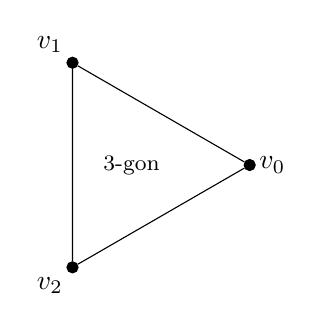
\begin{tikzpicture}[
      vtx/.style={
        circle, draw, fill=black,
        inner sep=0pt, minimum width=4pt
      }
    ]
      \foreach \ang/\x in {0/v0,120/v1,240/v2} {
        \node[vtx] (\x) at (\ang:1.5){};
      }
      \node[font=\footnotesize] at (0,0){$3$-gon};
      \node[right] at (v0){$v_0$};
      \node[above left] at (v1){$v_1$};
      \node[below left] at (v2){$v_2$};

      \draw (v0)--(v1)--(v2)--(v0);
    \end{tikzpicture}
    &
    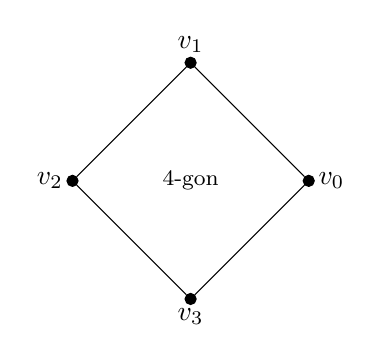
\begin{tikzpicture}[
      vtx/.style={
        circle, draw, fill=black,
        inner sep=0pt, minimum width=4pt
      }
    ]
      \foreach \ang/\x in {0/v0,90/v1,180/v2,270/v3} {
        \node[vtx] (\x) at (\ang:1.5){};
      }
      \node[font=\footnotesize] at (0,0){$4$-gon};
      \node[right] at (v0){$v_0$};
      \node[above] at (v1){$v_1$};
      \node[left] at (v2){$v_2$};
      \node[below] at (v3){$v_3$};

      \draw (v0)--(v1)--(v2)--(v3)--(v0);
    \end{tikzpicture}
    &
    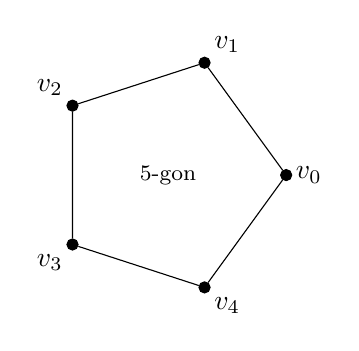
\begin{tikzpicture}[
      vtx/.style={
        circle, draw, fill=black,
        inner sep=0pt, minimum width=4pt
      }
    ]
      \foreach \ang/\x in {0/v0,72/v1,144/v2,216/v3,288/v4} {
        \node[vtx] (\x) at (\ang:1.5){};
      }
      \node[font=\footnotesize] at (0,0){$5$-gon};
      \node[right] at (v0){$v_0$};
      \node[above right] at (v1){$v_1$};
      \node[above left] at (v2){$v_2$};
      \node[below left] at (v3){$v_3$};
      \node[below right] at (v4){$v_4$};

      \draw (v0)--(v1)--(v2)--(v3)--(v4)--(v0);
    \end{tikzpicture}
    \\
  \end{tabular}
\end{center}

\begin{defn}{symmetry, dihedral group}{symmetry_dihedralgroup}
  A \hldef{symmetry} of the $n$-gon $P_n$ is an invertible linear transformation
  $T \in \GL_2(\R)$ such that $T(P_n) = P_n$.

  The set of symmetries of $P_n$ is called the \hldef{dihedral group} and is denoted by $D_{2n}$
  (or $D_n$).
\end{defn}

(Think of matrices and linear transformations interchangeably.
Matrix multiplication = composition of transformations.)

\begin{prop}{}{}
  $D_{2n}$ is a group under composition.
\end{prop}

Proof later (key point: $S, T \in D_{2n} \implies ST \in D_{2n}$).

\begin{lem}{}{}
  Say $v_i$ and $v_j$ are adjacent in $P_n$ if they are connected by a line segment.
  \begin{enumerate}
    \item If $T \in D_{2n}$, then $(T(v_0), T(v_1))$ are adjacent.
    \item If $S, T \in D_{2n}$ and $S(v_i) = T(v_i)$ for $i = 0, 1$, then $S = T$.
  \end{enumerate}
\end{lem}

\begin{thmproof}
  \begin{enumerate}
    \item $v_0, v_1$ are adjacent and $T$ is linear (lines map to lines).
    \item $v_0, v_1$ are linearly independent (and form a basis in $\R^2$).
  \end{enumerate}
\end{thmproof}

\begin{cor}{}{}
  $\abs{D_{2n}} \leq 2n$.
\end{cor}

\begin{thmproof}
  Let $A$ be the set of adjacent $(v_i, v_j)$, so $\abs{A} = 2n$.
  By lemma, $D_{2n} \to A : T \mapsto (T(v_0), T(v_1))$ is well-defined and injective.
\end{thmproof}

Intuitively, we can ask: for every pair of adjacent vertices $(v_i, v_j)$, is there an element
$T \in D_{2n}$ with $T(v_0) = v_i$ and $T(v_1) = v_j$?
If yes, then $\abs{D_{2n}} = 2n$.

\pagebreak
\subsection[Special elements of D2n]{Special elements of $D_{2n}$}

Let $s \in D_{2n}$ be rotation by $2\pi / n$ radians, so $\abs{s} = n$ (that is, $s^n = e$ and
$s^k \neq e$ for $1 \leq k < n$).

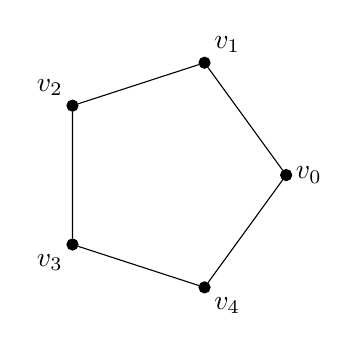
\begin{tikzpicture}[
  vtx/.style={
    circle, draw, fill=black,
    inner sep=0pt, minimum width=4pt
  }
]
  \foreach \ang/\x in {0/v0,72/v1,144/v2,216/v3,288/v4} {
    \node[vtx] (\x) at (\ang:1.5){};
  }
  \node[right] at (v0){$v_0$};
  \node[above right] at (v1){$v_1$};
  \node[above left] at (v2){$v_2$};
  \node[below left] at (v3){$v_3$};
  \node[below right] at (v4){$v_4$};
  \draw (v0)--(v1)--(v2)--(v3)--(v4)--(v0);
\end{tikzpicture}
\begin{tikzpicture}[
  vtx/.style={
    circle, draw, fill=black,
    inner sep=0pt, minimum width=4pt
  }
]
  \foreach \ang/\x in {0/v0,72/v1,144/v2,216/v3,288/v4} {
    \node[vtx] (\x) at (\ang:1.5){};
  }
  \node[right] at (v0){$v_1$};
  \node[above right] at (v1){$v_2$};
  \node[above left] at (v2){$v_3$};
  \node[below left] at (v3){$v_4$};
  \node[below right] at (v4){$v_0$};
  \draw (v0)--(v1)--(v2)--(v3)--(v4)--(v0);
  \draw[->] (-3,0)--(-2,0){} node[midway, above]{$s$};
  \node at (-3.25,0){};
\end{tikzpicture}
\begin{tikzpicture}[
  vtx/.style={
    circle, draw, fill=black,
    inner sep=0pt, minimum width=4pt
  }
]
  \foreach \ang/\x in {0/v0,72/v1,144/v2,216/v3,288/v4} {
    \node[vtx] (\x) at (\ang:1.5){};
  }
  \node[right] at (v0){$v_2$};
  \node[above right] at (v1){$v_3$};
  \node[above left] at (v2){$v_4$};
  \node[below left] at (v3){$v_0$};
  \node[below right] at (v4){$v_1$};
  \draw (v0)--(v1)--(v2)--(v3)--(v4)--(v0);
  \draw[->] (-3,0)--(-2,0){} node[midway, above]{$s$};
  \node at (-3.25,0){};
\end{tikzpicture}

\begin{tikzpicture}[
  vtx/.style={
    circle, draw, fill=black,
    inner sep=0pt, minimum width=4pt
  }
]
  \foreach \ang/\x in {0/v0,72/v1,144/v2,216/v3,288/v4} {
    \node[vtx] (\x) at (\ang:1.5){};
  }
  \node[right] at (v0){$v_3$};
  \node[above right] at (v1){$v_4$};
  \node[above left] at (v2){$v_0$};
  \node[below left] at (v3){$v_1$};
  \node[below right] at (v4){$v_2$};
  \draw (v0)--(v1)--(v2)--(v3)--(v4)--(v0);
  \draw[->] (-3,0)--(-2,0){} node[midway, above]{$s$};
\end{tikzpicture}
\begin{tikzpicture}[
  vtx/.style={
    circle, draw, fill=black,
    inner sep=0pt, minimum width=4pt
  }
]
  \foreach \ang/\x in {0/v0,72/v1,144/v2,216/v3,288/v4} {
    \node[vtx] (\x) at (\ang:1.5){};
  }
  \node[right] at (v0){$v_4$};
  \node[above right] at (v1){$v_0$};
  \node[above left] at (v2){$v_1$};
  \node[below left] at (v3){$v_2$};
  \node[below right] at (v4){$v_3$};
  \draw (v0)--(v1)--(v2)--(v3)--(v4)--(v0);
  \draw[->] (-3,0)--(-2,0){} node[midway, above]{$s$};
  \node at (-3.25,0){};
\end{tikzpicture}
\begin{tikzpicture}[
  vtx/.style={
    circle, draw, fill=black,
    inner sep=0pt, minimum width=4pt
  }
]
  \foreach \ang/\x in {0/v0,72/v1,144/v2,216/v3,288/v4} {
    \node[vtx] (\x) at (\ang:1.5){};
  }
  \node[right] at (v0){$v_0$};
  \node[above right] at (v1){$v_1$};
  \node[above left] at (v2){$v_2$};
  \node[below left] at (v3){$v_3$};
  \node[below right] at (v4){$v_4$};
  \draw (v0)--(v1)--(v2)--(v3)--(v4)--(v0);
  \draw[->] (-3,0)--(-2,0){} node[midway, above]{$s$};
  \node at (-3.25,0){};
\end{tikzpicture}

Let $r$ be reflection through the $x$-axis.

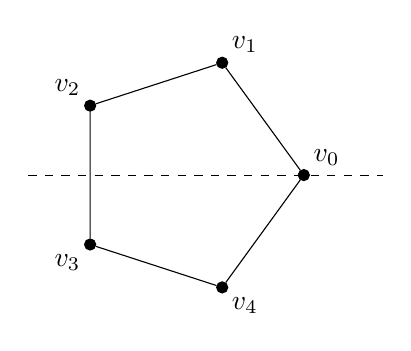
\begin{tikzpicture}[
  vtx/.style={
    circle, draw, fill=black,
    inner sep=0pt, minimum width=4pt
  }
]
  \foreach \ang/\x in {0/v0,72/v1,144/v2,216/v3,288/v4} {
    \node[vtx] (\x) at (\ang:1.5){};
  }
  \node[above right] at (v0){$v_0$};
  \node[above right] at (v1){$v_1$};
  \node[above left] at (v2){$v_2$};
  \node[below left] at (v3){$v_3$};
  \node[below right] at (v4){$v_4$};
  \draw (v0)--(v1)--(v2)--(v3)--(v4)--(v0);
  \draw[dashed] (-2,0)--(2.5,0);
\end{tikzpicture}
\begin{tikzpicture}[
  vtx/.style={
    circle, draw, fill=black,
    inner sep=0pt, minimum width=4pt
  }
]
  \foreach \ang/\x in {0/v0,72/v1,144/v2,216/v3,288/v4} {
    \node[vtx] (\x) at (\ang:1.5){};
  }
  \node[above right] at (v0){$v_0$};
  \node[above right] at (v1){$v_4$};
  \node[above left] at (v2){$v_3$};
  \node[below left] at (v3){$v_2$};
  \node[below right] at (v4){$v_1$};
  \draw (v0)--(v1)--(v2)--(v3)--(v4)--(v0);
  \draw[->] (-3,0)--(-2,0) node[midway, above]{$r$};
  \node at (-3.25,0){};
\end{tikzpicture}

$\abs{r} = 2$, that is, $r^2 = e$ and $r \neq e$.

We have $r(v_0) = v_0$ and $r(v_1)$ is now the vertex before $v_0$ rather than the vertex after.

\pagebreak
\subsection{Putting rotation and reflection together}

$s^i$ for $0 \leq i < n$ sends $v_0 \mapsto v_i$ and $v_1 \mapsto v_{i + 1}$.
(Say $v_n = v_0$ and $s^0 = e$.)

$s^i r$ for $0 \leq i < n$ sends $v_0 \mapsto v_i$ and $v_1 \mapsto v_{i - 1}$.
(Say $v_{-1} = v_{n - 1}$.)

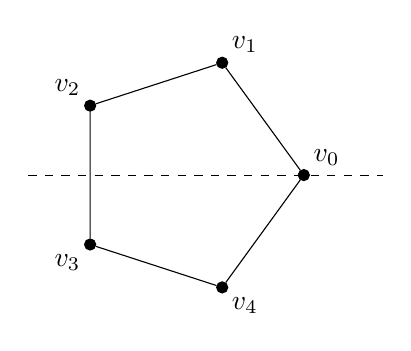
\begin{tikzpicture}[
  vtx/.style={
    circle, draw, fill=black,
    inner sep=0pt, minimum width=4pt
  }
]
  \foreach \ang/\x in {0/v0,72/v1,144/v2,216/v3,288/v4} {
    \node[vtx] (\x) at (\ang:1.5){};
  }
  \node[above right] at (v0){$v_0$};
  \node[above right] at (v1){$v_1$};
  \node[above left] at (v2){$v_2$};
  \node[below left] at (v3){$v_3$};
  \node[below right] at (v4){$v_4$};
  \draw (v0)--(v1)--(v2)--(v3)--(v4)--(v0);
  \draw[dashed] (-2,0)--(2.5,0);
\end{tikzpicture}
\begin{tikzpicture}[
  vtx/.style={
    circle, draw, fill=black,
    inner sep=0pt, minimum width=4pt
  }
]
  \foreach \ang/\x in {0/v0,72/v1,144/v2,216/v3,288/v4} {
    \node[vtx] (\x) at (\ang:1.5){};
  }
  \node[above right] at (v0){$v_0$};
  \node[above right] at (v1){$v_4$};
  \node[above left] at (v2){$v_3$};
  \node[below left] at (v3){$v_2$};
  \node[below right] at (v4){$v_1$};
  \draw (v0)--(v1)--(v2)--(v3)--(v4)--(v0);
  \draw[->] (-3,0)--(-2,0) node[midway, above]{$r$};
  \node at (-3.25,0){};
\end{tikzpicture}
\begin{tikzpicture}[
  vtx/.style={
    circle, draw, fill=black,
    inner sep=0pt, minimum width=4pt
  }
]
  \foreach \ang/\x in {0/v0,72/v1,144/v2,216/v3,288/v4} {
    \node[vtx] (\x) at (\ang:1.5){};
  }
  \node[above right] at (v0){$v_2$};
  \node[above right] at (v1){$v_1$};
  \node[above left] at (v2){$v_0$};
  \node[below left] at (v3){$v_4$};
  \node[below right] at (v4){$v_3$};
  \draw (v0)--(v1)--(v2)--(v3)--(v4)--(v0);
  \draw[->] (-3,0)--(-2,0) node[midway, above]{$s^2$};
  \node at (-3.25,0){};
\end{tikzpicture}

\begin{prop}{}{}
  $D_{2n} = \{ s^i r^j : 0 \leq i < n, \ 0 \leq j < 2 \}$, so $\abs{D_{2n}} = 2n$.
\end{prop}

So what is $rs$?

$rs(v_0) = r(v_1) = v_{n - 1}$ and $rs(v_1) = r(v_2) = v_{n - 2}$.

So $rs = s^{n - 1} r = s^{-1} r$.

\begin{cor}{}{}
  $D_{2n}$ is a finite non-abelian group.
\end{cor}

In summary:
\begin{itemize}
  \item $D_{2n} = \{ s^i r^j : 0 \leq i < n, \ 0 \leq j < 2 \}$
  \item $\abs{D_{2n}} = 2n$
  \item $s^n = e$, $r^2 = e$, $rs = s^{-1} r$
  \item $D_{2n}$ is a finite non-abelian group.
\end{itemize}
Exercise: show these relations are enough to completely determine $D_{2n}$.

\pagebreak
\subsection{What's group theory about?}

Basic answer: sets with one binary operation.

Better answer: group theory is the study of symmetry.

If we resize or rotate $P_n$, then the symmetries remain the same.

Kleinian view of geometry:
\begin{itemize}
  \item $D_{2n}$ captures what is means to be a regular $n$-gon.
  \item More generally, geometry is about the study of symmetries.
\end{itemize}

\pagebreak
\subsection{Permutation groups}

If $X$ is a set, let $\Fun(X, X)$ be the set of functions $X \to X$.
Then
\[ \circ \colon \Fun(X, X) \times \Fun(X, X) \to \Fun(X, X) : (f, g) \mapsto f \circ g \]
is an associative operation with an identity $\Id_X$.

Let $S_X = \{ f \in \Fun(X, X) : f \text{ is a bijection} \}$.

\begin{prop}{}{}
  $S_X$ is a group under $\circ$.
\end{prop}

\begin{thmproof}
  Homework.
\end{thmproof}

\begin{defn}{symmetric group}{symmetricgroup}
  Let $n \geq 1$.
  The \hldef{symmetric group} (or \hldef{permutation group}) $S_n$ is the group $S_X$ with
  $X = \{1, \ldots, n\}$.
\end{defn}

Elements of $S_n$ are bijections $\pi \colon \{1, \ldots, n\} \to \{1, \ldots, n\}$.

What makes such a $\pi$ a bijection?
Every element of $\{1, \ldots, n\}$ must appear in the list $\pi(1), \ldots, \pi(n)$ and no
element can appear twice.

We have $n$ choices for $\pi(1)$, $n - 1$ choices for $\pi(2)$, \dots, 1 choice for $\pi(n)$.
Thus $\abs{S_n} = n(n - 1) \cdots 1 = n!$.

Note $\abs{S_1} = 1! = 1$, so $S_1$ is the trivial group.

\pagebreak
\subsection{Permutations}

Elements of $S_n$ are called \hldef{permutations}.
We have several ways of representing permutations:
\begin{enumerate}
  \item
  Two-line representation:
  \[ \pi = \begin{pmatrix} 1 & 2 & 3 & 4 & 5 & 6 \\ 6 & 5 & 1 & 4 & 2 & 3 \end{pmatrix} \]
  \item
  One-line representation: $\pi = 651423$.
  \item
  Disjoint cycle representation: write down the \hldef{cycles} of $\pi$.
  Here $\pi(1) = 6$, $\pi(6) = 3$, and $\pi(3) = 1$, so $(163)$ is a cycle of $\pi$.

  $\pi = (163)(25)(4) = (163)(25)$.
  We typically drop cycles of length 1, and write cycles containing the smallest unused element
  first.

  The identity is empty in disjoint cycle notation, so we just use $e$.
\end{enumerate}

Multiplication can be done in two-line or disjoint cycle notation:
\begin{align*}
  \pi &= \begin{pmatrix}
    1 & 2 & 3 & 4 & 5 & 6 \\
    6 & 5 & 1 & 4 & 2 & 3
  \end{pmatrix} = (163)(25) \\
  \sigma &= \begin{pmatrix}
    1 & 2 & 3 & 4 & 5 & 6 \\
    2 & 6 & 4 & 5 & 3 & 1
  \end{pmatrix} = (126)(345) \\
  \pi\sigma &= \begin{pmatrix}
    1 & 2 & 3 & 4 & 5 & 6 \\
    5 & 3 & 4 & 2 & 1 & 6
  \end{pmatrix} = (15)(234)
\end{align*}
One-line notation is hard, so we don't use it here.

Inversion can also be done in two-line or disjoint cycle notation:
\[
  \pi = \begin{pmatrix}
    1 & 2 & 3 & 4 & 5 & 6 \\
    6 & 5 & 1 & 4 & 2 & 3
  \end{pmatrix} = (163)(25)
\]
\[
  \pi^{-1} = \begin{pmatrix}
    6 & 5 & 1 & 4 & 2 & 3 \\
    1 & 2 & 3 & 4 & 5 & 6
  \end{pmatrix} = \begin{pmatrix}
    1 & 2 & 3 & 4 & 5 & 6 \\
    3 & 5 & 6 & 4 & 2 & 1
  \end{pmatrix} = (136)(25)
\]
If $\pi(i) = j$, then $\pi^{-1}(j) = i$, so cycles of $\pi^{-1}$ are cycles of $\pi$ in reverse
order.

\pagebreak
\subsection{Fixed points and support sets}

\begin{defn}{fixed point, support set}{fixedpoint_supportset}
  The \hldef{fixed points} of a permutation $\pi \in S_n$ are the numbers $1 \leq i \leq n$ such
  that $\pi(i) = i$.

  The \hldef{support set} of $\pi \in S_n$ is
  \[ \supp(\pi) = \{ 1 \leq i \leq n : \pi(i) \neq i \}. \]

  $\pi$ and $\sigma$ are \hldef{disjoint} if $\supp(\pi) \cap \supp(\sigma) = \varnothing$.
\end{defn}

\begin{ex}
  $\supp((163)(25)) = \{1, 2, 3, 5, 6\}$.
\end{ex}

Some notes:
\begin{itemize}
  \item
  In general, $\supp(\pi)$ are exactly the numbers that appear in the disjoint cycle representation
  of $\pi$ (when length-1 cycles are omitted).
  \item
  $\supp(\pi) = \varnothing$ if and only if $\pi = e$.
  \item
  $\supp(\pi^{-1}) = \supp(\pi)$.
  \item
  If $i \in \supp(\pi)$, then $\pi(i) \in \supp(\pi)$.
\end{itemize}

\pagebreak
\subsection{Commuting elements}

\begin{defn}{commute}{commute}
  Two elements $g, h$ in a group $G$ \hldef{commute} if $gh = hg$.
\end{defn}

\begin{lem}{}{}
  If $\pi, \sigma \in S_n$ are disjoint, then $\pi\sigma = \sigma\pi$.
\end{lem}

\begin{thmproof}
  Suppose $1 \leq i \leq n$.

  If $i \in \supp(\pi)$, then $\pi(i) \in \supp(\pi)$.
  Since $\pi, \sigma$ are disjoint, we have $i, \pi(i) \not\in \supp(\sigma)$.
  So $\pi(\sigma(i)) = \pi(i) = \sigma(\pi(i))$.

  By symmetry, $\pi(\sigma(i)) = \sigma(\pi(i))$ if $i \in \supp(\sigma)$.

  If $i \not\in \supp(\pi) \cup \supp(\sigma)$, then $\pi(\sigma(i)) = i = \sigma(\pi(i))$.

  Then $\pi(\sigma(i)) = \sigma(\pi(i))$ for all $i$, so $\pi\sigma = \sigma\pi$.
\end{thmproof}

\pagebreak
\subsection{Cycles}

\begin{defn}{cycle}{cycle}
  A \hldef{$k$-cycle} is an element of $S_n$ with disjoint cycle notation $(i_1 i_2 \cdots i_k)$.
\end{defn}

Suppose the cycles of $\pi \in S_n$ are $c_1, \ldots, c_k$.
We can regard $c_i$ as an element of $S_n$ and $\pi = c_1 \cdot c_2 \cdot \cdots \cdot c_k$ as a
product in $S_n$.
Since $c_i$ and $c_j$ are disjoint, $c_i c_j = c_j c_i$.
Thus the order of cycles in disjoint cycle representation doesn't matter.

\begin{ex}
  $\pi = (163)(25) = (25) \cdot (163)$.
\end{ex}

Additionally, we have $\pi^{-1} = c_k^{-1} \cdots c_1^{-1} = c_1^{-1} \cdots c_k^{-1}$.

\begin{ex}
  If $c$ and $c'$ are non-disjoint cycles, then they don't necessarily commute:
  $(12)(23) = (123)$ while $(23)(12) = (123)^{-1} = (132) \neq (12)(23)$.
\end{ex}

If $\pi$ is a permutation, then $\pi$ commutes with $\pi^i$ for all $i$, so $\pi$ and $\pi^i$
commute.
However, $\pi$ and $\pi^i$ don't have disjoint support sets.

\week{Subgroups and Homomorphisms}

%%%%% Lec 3
\section{Subgroups}

\subsection{Subgroups}

\begin{defn}{subgroup}{subgroup}
  Let $(G, \cdot)$ be a group.
  A subset $H \subseteq G$ is a \hldef{subgroup} of $G$ if
  \begin{enumerate}
    \item for all $g, h \in H$, $g \cdot h \in H$ ($H$ is \hldef{closed under products}),
    \item for all $g \in H$, $g^{-1} \in H$ ($H$ is \hldef{closed under inverses}), and
    \item $e_G \in H$.
  \end{enumerate}

  Notation: $H \leq G$.
\end{defn}

\begin{ex}
  \begin{itemize}
    \item $\Z \leq \Q^+ := (\Q, +)$.
    \item $\Q_{> 0} := \{ x \in \Q : x > 0 \} \leq \Q^\times$.

    Check: if $x, y \in \Q$ and $x, y > 0$, then $xy > 0 \implies xy \in \Q_{> 0}$.
    Also, if $x > 0$, then $1/x > 0 \implies 1/x \in \Q_{> 0}$.
  \end{itemize}
\end{ex}

\begin{ex}
  Let $G = D_{2n}$ and $s$ be rotation.

  $H = \{ e = s^0, s, s^2, \ldots, s^{n - 1} \}$ is a subgroup of $D_{2n}$.
\end{ex}

\begin{exerproof}
  Claim: $s^i \in H$ for all $i \in \Z$.

  Proof: let $i = nk + r$ with $0 \leq r < n$.
  Then $s^i = s^{nk + r} = (s^n)^k s^r = s^r$ since $s^n = e$.

  Checking subgroup properties:
  \begin{itemize}
    \item If $s^i, s^j \in H$, then $s^{i + j} \in H$.
    \item If $s^i \in H$, then $s^{-i} \in H$.
    \item $e \in H$.
  \end{itemize}
\end{exerproof}

$H$ is the smallest subgroup containing $s$ (since subgroups are closed under products).

Notation for $H$ is $\ang{s}$.

\begin{ex}
  Let $G = \Z = (\Z, +)$.

  If $m \in \Z$, then
  $m\Z := \{ km : k \in \Z \} = \{ n \in \Z : m \mid n \}$ is a subgroup of
  $\Z$.

  In particular, $0\Z = \{0\}$ is a subgroup of $\Z$ called the \hldef{trivial
  subgroup}.
\end{ex}

\begin{defn}{trivial subgroup, proper subgroup}{trivialpropersubgroup}
  If $G$ is a group, then $\{e\}$ is a subgroup called the \hldef{trivial subgroup}.

  Also, $G$ is a subgroup of $G$.
  A subgroup $H$ is \hldef{proper} if $H \neq G$.
  Notation: $H < G$.
\end{defn}

$H$ is a proper non-trivial subgroup if $\{e\} \neq H < G$.

\begin{ex}
  Some non-subgroups:
  \begin{itemize}
    \item
    $\Q_{\geq 0} := \{x \in \Q : x \geq 0\}$ is not a subgroup of $\Q^+$.

    If $x, y \in \Q_{\geq 0}$, then $x + y \in \Q_{\geq 0}$.
    Also, $0 \in \Q_{\geq 0}$.

    But if $x \in Q_{\geq 0}$, then $-x \not\in \Q_{\geq 0}$ unless $x = 0$.
    \item
    $\Q^\times$ is not a subgroup of $(\Q, \cdot)$ because $(\Q, \cdot)$ is
    not a group.
  \end{itemize}
\end{ex}

\begin{prop}{}{}
  If $H$ is a subgroup of $(G, \boxtimes)$, then $(H, \boxtimes \rvert_{H \times H})$ is a group,
  such that
  \begin{enumerate}
    \item the identity of $H$ is $e_H = e_G$, and
    \item the inverse of $g \in H$ is the same as the inverse of $g$ in $G$.
  \end{enumerate}
\end{prop}

\begin{thmproof}
  First, we show $\boxtimes \rvert_{H \times H}$ is a binary operation on $H$.
  Note $\boxtimes$ is a function $G \times G \to G$, so $\boxtimes \rvert_{H \times H}$ is a
  function $H \times H \to G$.
  But if $g, h \in H$, then $g \boxtimes h \in H$.
  Thus $\boxtimes \rvert_{H \times H}$ is a function $H \times H \to H$.

  From now on, denote this function by $\tilde{\boxtimes}$.

  Since $\boxtimes$ is associative, $\tilde{\boxtimes}$ is associative.

  Note $e_H = e_G$ is the identity for $\tilde{\boxtimes}$.

  If $g \in H$, then $g^{-1}$ with respect to $\boxtimes$ is in $H$.

  Since $g \mathop{\tilde{\boxtimes}} g^{-1} = g^{-1} \mathop{\tilde{\boxtimes}} g = e_G = e_H$,
  $g^{-1}$ is the inverse of $g$ with respect to $\tilde{\boxtimes}$.

  So $(H, \tilde{\boxtimes})$ is a group.
\end{thmproof}

We call $\tilde{\boxtimes}$ the \hldef{operation induced by $\boxtimes$} on $H$.
Usually we just refer to $\tilde{\boxtimes}$ as $\boxtimes$.

\begin{ex}
  \begin{itemize}
    \item $\Z$ is a subgroup of $\Q$ with operation $+$.
    \item If $H$ is a subgroup of $(G, \cdot)$, then $H$ is a group with operation $\cdot$.
  \end{itemize}
\end{ex}

\pagebreak
\subsection{Speeding up the subgroup check}

\begin{prop}{}{}
  $H$ is a subgroup of $G$ if and only if
  \begin{enumerate}
    \item $H$ is non-empty, and
    \item $gh^{-1} \in H$ for all $g, h \in H$.
  \end{enumerate}
\end{prop}

\begin{thmproof}
  \begin{enumerate}[leftmargin=4em]
    \item[($\implies$)]
    If $H$ is a subgroup of $G$, then $e_G \in H$, so $H \neq \varnothing$.
    Also if $g, h \in H$, then $h^{-1} \in H$ and $gh^{-1} \in H$.
    \item[($\impliedby$)]
    By (1), there is some $x \in H$.
    By (2), $xx^{-1} = e_G \in H$.

    Also by (2), $e_G \cdot x^{-1} = x^{-1} \in H$ (so $H$ is closed under inverses).

    Now if $x, y \in H$, then $y^{-1} \in H$, so $xy = x(y^{-1})^{-1} \in H$ (so $H$ is closed under
    products).
  \end{enumerate}
\end{thmproof}

\begin{ex}
  Let $(V, +, \cdot)$ be a vector space.

  If $W$ is a subspace of $V$, then $W$ is a subgroup of $(V, +)$.

  Check:
  \begin{itemize}
    \item $0 \in W$ so $W$ is non-empty.
    \item If $v, w \in W$, then $v + (-w) = v - w \in W$.
  \end{itemize}
  $W$ is a subgroup by the proposition.
\end{ex}

\pagebreak
\subsection{Finite subgroups}

\begin{prop}{}{}
  Suppose $H$ is a finite subset of $G$.
  Then $H$ is a subgroup of $G$ if and only if
  \begin{enumerate}
    \item $H$ is non-empty, and
    \item $gh \in H$ for all $g, h \in H$.
  \end{enumerate}
\end{prop}

\begin{thmproof}
  The forward direction is trivial.

  Suppose $g \in H$.
  By induction, we can show $g^n \in H$ for all $n \in \N$.

  Since $H$ is finite, the sequence $g, g^2, g^3, \ldots \in H$ must eventually repeat.

  So $g^i = g^j$ for some $1 \leq i < j \implies g^n = e$ for $n = j - i$.

  If $n = 1$, then $g^n = g = e$ so $g^{-1} = e \in H$.
  If $n > 1$, then $g^{n - 1} = g^{-1} \in H$.
\end{thmproof}

\pagebreak
\subsection{Subgroups generated by a set}

\begin{prop}{}{}
  Suppose $\mathcal{F}$ is a non-empty set of subgroups of $G$.
  Then
  \[ K := \bigcap_{H \in \mathcal{F}} H \]
  is a subgroup of $G$.
\end{prop}

\begin{thmproof}
  Note $e_G \in H$ for all $H \in \mathcal{F}$, so $e_G \in K$ and thus $K$ is non-empty.

  Now consider $x, y \in K$.
  Then $x, y \in H$ for all $H \in \mathcal{F}$, so $y^{-1} \in H$ for all $H \in \mathcal{F}$,
  so $xy^{-1} \in H$ for all $H \in \mathcal{F}$, so $xy^{-1} \in K$.

  By proposition, $K$ is a subgroup of $G$.
\end{thmproof}

\begin{defn}{subgroup generated by a set}{subgroupgenerated}
  Let $S$ be a subset of a group $G$.

  The \hldef{subgroup generated by $S$ in $G$} is
  \[ \ang{S} := \bigcap_{S \subseteq H \leq G} H. \]
\end{defn}

Notes:
\begin{itemize}
  \item The intersection is non-empty because $S \subseteq G \leq G$.
  \item If $S \subseteq K \leq G$, then $\ang{S} \subseteq K$.
  So say that $\ang{S}$ is the smallest subgroup of $G$ containing $S$.
  \item $\ang{\varnothing} = \ang{e} = \{e\}$, the trivial subgroup.
  \item If $S = \{s_1, s_2, \ldots\}$, we often write
  $\ang{S} = \ang{s_1, s_2, \ldots}$.
\end{itemize}

\begin{ex}
  Consider $D_{2n}$ and its rotation generator $s$.

  Let $K = \{e = s^0, s^1, s^2, \ldots, s^{n - 1}\}$.
  As previously checked, $K$ is a subgroup of $D_{2n}$.

  Since $s \in K$, $\ang{s} \in K$.

  On the other hand, we can show by induction that $s^i \in \ang{s}$ for all
  $i \in \Z$.
  So $K \subseteq \ang{s} \implies \ang{s} = K$.
\end{ex}

Note that $\ang{s}$ is constructed by taking all products of $s$ with itself.
Can we generalize this example?

If $S \subset G$, let $S^{-1} = \{s^{-1} : s \in S\}$.

\begin{prop}{}{}
  If $S \subset G$, let
  \[ K = \{e\} \cup \{ s_1 \cdots s_k : k \geq 1, \ s_1, \ldots, s_k \in S \cup S^{-1} \}. \]
  Then $\ang{S} = K$.
\end{prop}

\begin{thmproof}
  Claim 1: $S \subseteq K \subseteq \ang{S}$.

  Proof: We know $e \in \ang{S}$.
  Prove by induction that $s_1 \cdots s_k \in \ang{S}$ for all $k \geq 1$ and
  $s_1, \ldots, s_k \in S \cup S^{-1}$.

  Claim 2: $K$ is a subgroup.

  Proof: $e \in K$ by construction.
  Consider $x, y \in K$.
  Then
  \begin{align*}
    x &= s_1 \cdots s_k, \ k \geq 0, \ s_1, \ldots, s_k \in S \cup S^{-1} \\
    y &= t_1 \cdots t_\ell, \ \ell \geq 0, \ t_1, \ldots, t_\ell \in S \cup S^{-1}.
  \end{align*}
  So $xy = s_1 \cdots s_k t_1 \cdots t_\ell \in K$, and $x^{-1} = s_k^{-1} \cdots s_1^{-1} \in K$
  since $s_k^{-1}, \ldots, s_1^{-1} \in S \cup S^{-1}$.

  So $K$ is a subgroup.

  Proof of proposition: $S \subseteq K$ and $\ang{S}$ is the smallest subgroup containing
  $S$, so $\ang{S} \subseteq K$.

  Thus $\ang{S} = K$.
\end{thmproof}

\pagebreak
\subsection{Lattice of subgroups}

Subgroups of $G$ are ordered by set inclusion $\subseteq$.

If $H_1, H_2 \leq G$ and $H_1 \subseteq H_2$, then $H_1 \leq H_2$, so we also write this order as
$\leq$.
(Exercise.)

The set of subgroups of $G$ with order $\leq$ is called the \hldef{lattice of subgroups of $G$}.

The first subgroup below $H_1, H_2 \leq G$ in the lattice is $H_1 \cup H_2$.
The first subgroup above $H_1, H_2 \leq G$ in the lattice is $\ang{H_1 \cup H_2}$.

\begin{center}
  \begin{forest}
    [$\Z$, calign=child, calign child=2
      [$2\Z$, name=2
        [$4\Z$, name=4]
      ]
      [$3\Z$
        [$6\Z$, name=6
          [$\vdots$, name=vdots
            [$0\Z$]
          ]
        ]
      ]
      [$\cdots$]
    ]
    \draw (2)--(6);
    \draw (4)--(vdots);
  \end{forest}
\end{center}

%%%%% Lec 4
\section{Cyclic groups}

\subsection{Generators and cyclic groups}

\begin{defn}{generate, cyclic}{}
  A subset $S$ of a group $G$ \hldef{generates} $G$ if $\ang{S} = G$.

  A group $G$ is \hldef{cyclic} if $G = \ang{a}$ for some $a \in G$.
\end{defn}

\begin{ex}
  \begin{itemize}
    \item $\Z = \ang{1} = \ang{-1}$ (generators are not unique)
    \item $\Zmod{n} = \ang{[1]} = \ang{[-1]}$
    \item $\Q^+$ is not cyclic (homework)
    \item If $G$ is a group, then $\ang{a}$ is a cyclic group for any $a \in G$ (called the
    \hldef{cyclic subgroup generated by $a$}).
  \end{itemize}
\end{ex}

\begin{lem}{}{}
  \begin{enumerate}
    \item If $a \in G$, then $\ang{a} = \{ a^i : i \in \Z \}$.
    \item If $\abs{a} = n$, then $\ang{a} = \{ a^i : 0 \leq i < n \}$.
  \end{enumerate}
\end{lem}

\begin{thmproof}
  \begin{enumerate}
    \item Follows from previous proposition about $\ang{S}$.
    \item See argument for $\ang{s}$ in $D_{2n}$.
  \end{enumerate}
\end{thmproof}

Questions:
\begin{itemize}
  \item In (2), can $\abs{\ang{a}}$ be smaller than $n$?
  \item Does $\abs{\ang{a}}$ determine $\abs{a}$?
\end{itemize}

\pagebreak
\subsection{Order of cyclic groups}

\begin{prop}{}{}
  If $G = \ang{a}$, then $\abs{G} = \abs{a}$.
\end{prop}

\begin{thmproof}
  We've already seen that $\abs{G} \leq \abs{a}$.

  Suppose $\abs{G} = n < \infty$.

  The sequence $a^0, a^1, a^2, \ldots, a^n \in G$ must have repetition.
  So there are $0 \leq i < j \leq n$ with $a^i = a^j$, which means $a^{j - i} = e$ and hence
  $\abs{a} \leq n$.

  So $\abs{a} \leq \abs{G}$, thus $\abs{a} = \abs{G}$.
\end{thmproof}

\pagebreak
\subsection{Examples in closer detail}

\begin{ex}
  For $G = \Z$:
  \begin{itemize}
    \item Infinite cyclic group.
    \item Generators: $+1$ and $-1$.
    \item Order of $m \in \Z$ is
    \[ \abs{m} = \begin{cases}
      \infty \qquad & m \neq 0 \\
      1 & m = 0
    \end{cases}. \]
    \item Cyclic subgroups are $\ang{m} = m\Z = \{ km : k \in \Z \}$.
    (Note difference in $\ang{a}$ between additive and multiplicative notation.)

    Homework: all subgroups of $\Z$ are cyclic.
  \end{itemize}
\end{ex}

\begin{ex}
  Can we analyze $\Zmod{n}$ in the same way?

  (Note: at this point we may drop the brackets. For example, in $\Zmod{5}$, $3 = 8$.)

  Questions:
  \begin{itemize}
    \item What are the generators of $\Zmod{n}$?
    \item What are the orders of elements of $\Zmod{n}$?
    \item What are the subgroups?
  \end{itemize}
\end{ex}

\pagebreak
\subsection[Generators of Z/nZ]{Generators of $\Zmod{n}$}

\begin{lem}{}{}
  Suppose $G = \ang{S}$.
  Then $G = \ang{T}$ if and only if $S \subseteq \ang{T}$.
\end{lem}

So $\Zmod{n} = \ang{[a]}$ if and only if $[1] \in \ang{[a]}$ (since $[1]$ is a
generator).
Note then
\begin{align*}
  [1] \in \ang{[a]} &\iff xa = 1 \pmod{n} \qquad \text{for some } x \in \Z \\
  &\iff xa - 1 = yn \qquad \text{for some } x, y \in \Z \\
  &\iff xa + yn = 1 \qquad \text{for some } x, y \in \Z \\
  &\iff \gcd(a, n) = 1
\end{align*}
so $\ang{[a]} = \Zmod{n}$ if and only if $\gcd(a, n) = 1$.

\pagebreak
\subsection[Order of elements in Z/nZ]{Order of elements in $\Zmod{n}$}

\begin{lem}{}{}
  If $G$ is a group, $g \in G$, and $g^n = e$, then $\abs{g} \mid n$.
\end{lem}

\begin{thmproof}
  Homework.
\end{thmproof}

If $a \in \Z$, then $n[a] = 0$, so $\abs{[a]} \mid n$.

\begin{lem}{}{}
  Suppose $a \mid n$.
  Then $\abs{[a]} = \frac{n}{a}$.
\end{lem}

\begin{thmproof}
  If $n = ka$, then $\ell[a] \neq 0$ for $1 \leq \ell < k$ and $k[a] = [ka] = 0$, so
  $\abs{[a]} = k$.
\end{thmproof}

\begin{lem}{}{}
  Suppose $a \in \Z$ and let $b = \gcd(a, n)$.
  Then $\ang{[a]} = \ang{[b]}$.
\end{lem}

\begin{thmproof}
  Since $b \mid a$, there is $k$ such that $a = kb$.
  Thus $[a] \in \ang{[b]}$, so $\ang{[a]} \subseteq \ang{[b]}$.

  By properties of $\gcd$, there are $x, y \in \Z$ such that $xa + yn = b$.

  So $[b] = x[a] + y[n] = x[a]$, which implies $[b] \in \ang{[a]}$ and thus
  $\ang{[b]} \subseteq \ang{[a]}$.

  Hence $\ang{[a]} = \ang{[b]}$.
\end{thmproof}

\begin{prop}{}{}
  Suppose $a \in \Z$.
  Then
  \[ \abs{[a]} = \frac{n}{\gcd(a, n)}. \]
\end{prop}

\begin{thmproof}
  Let $b = \gcd(a, n)$.
  Then $\ang{[a]} = \ang{[b]}$.
  So
  \[ \abs{[a]} = \abs{\ang{[a]}} = \abs{\ang{[b]}} = \abs{[b]}. \]
  But $b \mid n$, so by lemma $\abs{[b]} = \frac{n}{b}$.
\end{thmproof}

\pagebreak
\subsection[Subgroups of Z mod nZ]{Subgroups of $\Zmod{n}$}

\begin{cor}{}{}
  Let $n \geq 1$.
  \begin{itemize}
    \item The order $d$ of any cyclic subgroup of $\Zmod{n}$ divides $n$.
    \item For every $d \mid n$, there is a unique cyclic subgroup of $\Zmod{n}$ of order $d$.
    It is generated by $[a]$, where $a = \frac{n}{d}$.
  \end{itemize}
\end{cor}

\begin{thmproof}
  If $\abs{\ang{[a]}} = d$, then $d = \abs{[a]} \mid n$ by lemma.

  Also, $d = \frac{n}{\gcd(a, n)}$, and by lemma, $\ang{[a]} = \ang{[\frac{n}{d}]}$.

  Conversely, if $d \mid n$ and $a = \frac{n}{d}$, then $\abs{\ang{[a]}} = d$.
\end{thmproof}

\begin{ex}
  Cyclic subgroups of $\Zmod{6}$:
  \begin{itemize}
    \item $\ang{6} = \{0\}$.
    \item $\ang{3} = \{0, 3\}$.
    \item $\ang{2} = \{0, 2, 4\} = \ang{4}$.
    \item $\ang{1} = \{0, 1, 2, 3, 4, 5\} = \Zmod{6} = \ang{5}$.
  \end{itemize}

  Cyclic subgroups of $\Zmod{p}$ where $p$ prime:
  \begin{itemize}
    \item $\ang{p} = \ang{0}$.
    \item $\ang{1} = \Zmod{p}$.
  \end{itemize}
\end{ex}

\pagebreak
\subsection{Proofs later}

\begin{itemize}
  \item Every subgroup of a cyclic group is cyclic.
  (So the previous corollary is a complete list of subgroups of $\Zmod{n}$.)
  \item Every cyclic group is isomorphic to one of $\Zmod{n}$ for $n \geq 1$, or $\Z$.
\end{itemize}

%%%%% Lec 5
\section{Homomorphisms}

\subsection{Homomorphisms}

\begin{defn}{homomorphism (morphism)}{homomorphism}
  Let $G$ and $H$ be groups.
  A function $\phi \colon G \to H$ is a \hldef{homomorphism} (or \hldef{morphism}) if
  \[ \phi(g \cdot h) = \phi(g) \cdot \phi(h) \]
  for all $g, h \in G$.
\end{defn}

A homomorphism preserves the group operation from $G$ to $H$.

\begin{ex}
  \begin{itemize}
    \item
    For $\mathbb{K}$ a field, $\mathbb{K}^\times = \{a \in \mathbb{K} : a \neq 0\}$ is a group with
    operation $\cdot$.

    Then $\GL_n \mathbb{K} \to \mathbb{K}^\times : A \mapsto \det(A)$ is a homomorphism because
    $\det(AB) = \det(A) \det(B)$ for all $A, B$.
    \item
    Let $\R_{> 0} = \{x \in \R : x > 0\} \leq \R^\times$.
    Then $\R_{> 0} \to \R_{> 0} : x \mapsto \sqrt{x}$ is a homomorphism since
    $\sqrt{xy} = \sqrt{x} \sqrt{y}$.
    \item
    Additive notation: $\phi \colon (G, +) \to (H, +)$ is a homomorphism if
    $\phi(x + y) = \phi(x) + \phi(y)$ for all $x, y \in G$.

    $\phi \colon \Z \to \Z : k \mapsto mk$ is a homomorphism for any
    $m \in \Z$ since $\phi(x + y) = m(x + y) = mx + my = \phi(x) + \phi(y)$ for all
    $x, y \in \Z$.
    \item
    If $V, W$ are vector spaces and $T \colon V \to W$ is a linear transformation, then $T$ is a
    homomorphism from $(V, +)$ to $(W, +)$ since $T(v + w) = T(v) + T(w)$ for all $v, w \in V$.
    \item
    Mixed notation: $\R^+ \to \R^\times : x \mapsto e^x$ is a homomorphism since
    $e^{x + y} = e^x \cdot e^y$ for all $x, y \in \R^+$.
    \item
    $\R^+ \to \R^+ : x \mapsto e^x$ is not a homomorphism because
    $e^{x + y} \neq e^x + e^y$ in general (take $x = y = 0$).
  \end{itemize}
\end{ex}

\begin{lem}{}{}
  Suppose $\phi \colon G \to H$ is a homomorphism.
  Then:
  \begin{enumerate}
    \item $\phi(e_G) = e_H$.
    \item $\phi(g^{-1}) = \phi(g)^{-1}$ for all $g \in G$.
    \item $\phi(g^n) = \phi(g)^n$ for all $n \in \Z$.
    \item $\abs{\phi(g)} \mid \abs{g}$ for all $g \in G$ (say $n \mid \infty$ for all
    $n \in \N$).
  \end{enumerate}
\end{lem}

\begin{thmproof}
  \begin{enumerate}
    \item
    $\phi(e_G) = \phi(e_G^2) = \phi(e_G) \cdot \phi(e_G)$, so
    $e_H = \phi(e_G)^{-1} \cdot \phi(e_G) = \phi(e_G)^{-1} \cdot \phi(e_G) \cdot \phi(e_G)
      = \phi(e_G)$.
    \item
    $e_H = \phi(e_G) = \phi(gg^{-1}) = \phi(g) \phi(g^{-1})$ and similarly
    $\phi(g^{-1}) \phi(g) = e_H$, so $\phi(g^{-1})$ is the unique inverse of $\phi(g)$.
    \item
    Use induction for $n \geq 0$, additionally with part (b) for $n < 0$.
    \item
    If $\abs{g} = n < \infty$, then $g^n = e_G$ so $\phi(g)^n = \phi(g^n) = \phi(e_G) = e_H$.
    Homework: prove $\abs{\phi(g)} \mid n$.
  \end{enumerate}
\end{thmproof}

\pagebreak
\subsection{Making new homomorphisms from old}

\begin{lem}{}{}
  If $H \leq G$ and $H$ is considered as a group with the induced operation from $G$, then
  $i \colon H \to G : x \mapsto x$ is a homomorphism.
\end{lem}

\begin{thmproof}
  $i(g \cdot h) = g \cdot h = i(g) \cdot i(h)$.
\end{thmproof}

\begin{lem}{}{}
  If $\phi \colon G \to M$ and $\psi \colon H \to K$ are homomorphisms, then $\psi \circ \phi$ is
  a homomorphism.
\end{lem}

\begin{thmproof}
  $(\psi \circ \phi)(g \cdot h) = \psi(\phi(g) \cdot \phi(h)) = \psi(\phi(g)) \cdot \psi(\phi(h))$.
\end{thmproof}

\begin{cor}{}{}
  If $\phi \colon G \to H$ is a homomorphism and $K \leq G$, then the \hldef{restriction}
  $\phi \rvert_K$ is a homomorphism.
\end{cor}

\begin{thmproof}
  $\phi \rvert_K = \phi \circ i$, where $i \colon K \to G$ is the inclusion $x \mapsto x$.
\end{thmproof}

\pagebreak
\subsection{Images of homomorphisms}

If $f \colon X \to Y$ is a function and $S \subseteq X$, then say $f(S) := \{ f(x) : x \in S \}$.

\begin{prop}{}{}
  If $\phi \colon G \to H$ is a homomorphism and $K \leq G$, then $\phi(K) \leq H$.
\end{prop}

That is, homomorphisms send subgroups of the domain to subgroups of the codomain.

\begin{thmproof}
  Since $K$ is non-empty, $\phi(K)$ is non-empty.

  If $x, y \in \phi(K)$, then $x = \phi(x_0)$ and $y = \phi(y_0)$ for some $x_0, y_0 \in K$.

  So $xy^{-1} = \phi(x_0)\phi(y_0)^{-1} = \phi(x_0)\phi(y_0^{-1}) = \phi(x_0 y_0^{-1}) \in \phi(K)$,
  since $x_0 y_0^{-1} \in K$.
\end{thmproof}

\begin{defn}{image}{image}
  If $\phi \colon G \to H$ is a homomorphism, the \hldef{image} of $\phi$ is the subgroup
  $\Im \phi = \phi(G) \leq H$.
\end{defn}

\begin{ex}
  \begin{itemize}
    \item
    Let $\phi \colon \R^+ \to \R^\times : x \mapsto e^x$.

    $e^x > 0$ for all $x \in \R$, so $\Im \phi \subseteq \R_{> 0}$.

    If $y \in \R_{> 0}$, then $y = \phi(\log y)$, so $\Im \phi = \R_{> 0}$.
    \item
    If $K \leq G$ and $i \colon K \to G$ is inclusion, then $\Im i = K$.
    \item
    For $\phi \colon \Z \to \Z : k \mapsto mk$ for some $m \in \Z$,
    $\phi(\Z) = m\Z$.
  \end{itemize}
\end{ex}

\pagebreak
\subsection{Properties of images}

\begin{lem}{}{}
  If $\phi \colon G \to H$ is a homomorphism with $\Im \phi \leq K \leq H$, then the function
  $\tilde{\phi} \colon G \to K : x \mapsto \phi(x)$ is also a homomorphism with
  $\Im \tilde{\phi} = \Im \phi \leq K$.
\end{lem}

\begin{thmproof}
  \begin{align*}
    \tilde{\phi}(x \cdot y) &= \phi(x \cdot y) \\
    &= \phi(x) \cdot \phi(y) \qquad \text{in } H \\
    &= \tilde{\phi}(x) \cdot \tilde{\phi}(y) \qquad \text{in } K.
  \end{align*}

  Also $\tilde{\phi}(G) = \phi(G)$, regarded as a subset of $K$.
\end{thmproof}

We usually just refer to $\tilde{\phi}$ as $\phi$.

\begin{lem}{}{}
  A homomorphism $\phi \colon G \to H$ is surjective if and only if $\Im \phi = H$.
\end{lem}

\begin{thmproof}
  Obvious from definition.
\end{thmproof}

\begin{cor}{}{}
  $\phi$ induces a surjective homomorphism $\tilde{\phi} \colon G \to K$, where $K = \Im \phi$.
\end{cor}

\begin{prop}{}{}
  Let $\phi \colon G \to H$ be a homomorphism.
  If $S \subseteq G$, then $\phi(\ang{S}) = \ang{\phi(S)}$.
\end{prop}

\begin{thmproof}
  First, $\phi(S^{-1}) = \{\phi(s^{-1}) : s \in S\} = \{\phi(s)^{-1} : s \in S\} = \phi(S)^{-1}$.
  Thus
  \begin{align*}
    \phi(\ang{S})
    &= \phi(\{ s_1 \cdots s_k : k \geq 0, \ s_1, \ldots, s_k \in S \cup S^{-1} \}) \\
    &= \{ \phi(s_1) \cdots \phi(s_k) : k \geq 0, \ s_1, \ldots, s_k \in S \cup S^{-1} \} \\
    &= \{ t_1 \cdots t_k : k \geq 0, \ t_1, \ldots, t_k \in \phi(S) \cup \phi(S)^{-1} \} \\
    &= \ang{\phi(S)}.
  \end{align*}
\end{thmproof}

\pagebreak
\subsection{Pulling back subgroups}

If $f \colon X \to Y$ is a function and $S \subseteq Y$, then say
$f^{-1}(S) := \{x \in X : f(x) \in S\}$.

\begin{prop}{}{}
  If $\phi \colon G \to H$ is a homomorphism and $K \leq H$, then $\phi^{-1}(K) \leq G$.
\end{prop}

That is, we can also get a subgroup of the domain from a subgroup of the codomain.

Note: the forward and backward processes are not necessarily inverses, so we don't have a bijection
(just yet).

\begin{thmproof}
  $\phi(e_G) = e_H \in K$, so $e_G \in \phi^{-1}(K)$.

  If $x, y \in \phi^{-1}(K)$, then $\phi(x), \phi(y) \in K$ so
  $\phi(x y^{-1}) = \phi(x) \phi(y)^{-1} \in K$ and hence $xy^{-1} \in \phi^{-1}(K)$.
\end{thmproof}

\pagebreak
\subsection{The kernel of a homomorphism}

\begin{defn}{kernel}{kernel}
  If $\phi \colon G \to H$ is a homomorphism, then the \hldef{kernel} of $\phi$ is the subgroup
  $\ker \phi := \phi^{-1}(\{e_H\}) = \{ g \in G : \phi(g) = e_H \} \leq G$.
\end{defn}

\begin{ex}
  \begin{itemize}
    \item
    For $\det \colon \GL_n(\mathbb{K}) \to \mathbb{K}^\times$, we have
    $\ker \det = \{ A \in \GL_n(\mathbb{K}) : \det(A) = 1 \}$.

    This subgroup of $\GL_n(\mathbb{K})$ is called the \hldef{special linear group}, denoted by
    $\SL_n(\mathbb{K})$.
    \item
    If $\phi \colon \Z \to \Z : k \mapsto mk$, then $\phi(k) = 0$ if and only if
    $mk = 0$, so
    \[ \ker \phi = \begin{cases}
      \{0\} \qquad & m \neq 0 \\
      \Z & m = 0
    \end{cases}. \]
    \item
    If $\phi \colon \R^+ \to \R^\times : x \mapsto e^x$, then $e^x = 1$ if and only
    if $x = 0$, so $\ker \phi = \{0\}$.
  \end{itemize}
\end{ex}

\begin{prop}{}{}
  A homomorphism $\phi \colon G \to H$ is injective if and only if $\ker \phi = \{e_G\}$.
\end{prop}

\begin{thmproof}
  \begin{enumerate}[leftmargin=4em]
    \item[($\implies$)]
    If $\phi$ is injective, then $\phi(x) = e_H = \phi(e_G)$ if and only if $x = e_G$, so
    $\ker \phi = \{e_G\}$.
    \item[($\impliedby$)]
    Suppose $\ker \phi = \{e_G\}$ and $\phi(x) = \phi(y)$.

    Then $\phi(xy^{-1}) = \phi(x)\phi(y)^{-1} = e_H$, so $xy^{-1} \in \ker \phi$.

    But then $xy^{-1} = e_G$, so $x = y$.
    That is, $\phi$ is injective.
  \end{enumerate}
\end{thmproof}

\pagebreak
\subsection{Application: subgroups of cyclic groups}

\begin{prop}{}{}
  If $H$ is a subgroup of a cyclic group $G$, then $H$ is cyclic.
\end{prop}

\begin{thmproof}
  We need the following facts:
  \begin{enumerate}
    \item All subgroups of $\Z$ are of the form $m\Z = \ang{m}$, hence cyclic.
    (Homework.)
    \item $G$ is cyclic if and only if there is a surjective homomorphism $\Z \to G$.
    (Homework.)
    \item If $f \colon X \to Y$ is a surjective function and $S \subseteq Y$, then
    $f(f^{-1}(S)) = S$.
    (Exercise.)
  \end{enumerate}

  Since $G$ is cyclic, by (2) there is a surjective homomorphism $\phi \colon \Z \to G$.

  By (1), since all subgroups of $\Z$ are cyclic, there is $m \in \Z$ such that
  $\phi^{-1}(H) = \ang{m}$.

  So let $\psi \colon \Z \to \Z$ be the homomorphism with $\psi(k) = mk$.

  Then $\phi \circ \psi \colon \Z \to G$ is a homomorphism.
  We see that
  \[ (\phi \circ \psi)(\Z) = \phi(m\Z) = \phi(\phi^{-1}(H)) = H \]
  by (3).

  We can restrict the codomain of $\phi \circ \psi$ to get a surjective homomorphism
  $\Z \to H$.
  Hence $H$ is cyclic by (2).
\end{thmproof}

\pagebreak
\subsection{Review on bijections}

\begin{defn}{bijection}{bijection}
  Let $f \colon X \to Y$ be a function.
  Then $f$ is:
  \begin{itemize}
    \item \hldef{injective} if for all $x_1, x_2 \in X$, $f(x_1) = f(x_2)$ implies that $x_1 = x_2$;
    \item \hldef{surjective} if for all $y \in Y$, there exists $x \in X$ with $f(x) = y$; and
    \item \hldef{bijective} if $f$ is both injective and surjective.
  \end{itemize}
\end{defn}

\begin{prop}{}{}
  $f \colon X \to Y$ is a bijection if and only if there is a function $g \colon Y \to X$ such that
  $f \circ g = 1_Y$ and $g \circ f = 1_X$.
\end{prop}

If $g$ exists, then it is unique, and we denote it by $f^{-1}$.

\pagebreak
\subsection{Isomorphisms}

\begin{defn}{isomorphism}{isomorphism}
  A homomorphism $\phi \colon G \to H$ is an \hldef{isomorphism} if $\phi$ is a bijection.
\end{defn}

\begin{lem}{}{}
  $\phi \colon G \to H$ is an isomorphism if and only if $\ker \phi = \{e_G\}$ and $\Im \phi = H$.
\end{lem}

\begin{ex}
  \begin{itemize}
    \item $\R^+ \to \R_{> 0} : x \mapsto e^x$ is an isomorphism.
    \item If $\phi \colon G \to H$ is injective, then $\phi$ induces an isomorphism $G \to \Im\phi$.
    \item $\Z \to m\Z : k \mapsto mk$ is an isomorphism.
  \end{itemize}
\end{ex}

\begin{prop}{}{}
  Suppose $\phi \colon G \to H$ is an isomorphism.
  Then $\phi^{-1} : H \to G$ is also an isomorphism.
\end{prop}

\begin{thmproof}
  $\phi^{-1}$ is also a bijection, so we just need to show that it is a homomorphism.

  Let $g, h \in H$.
  Then $\phi(\phi^{-1}(g) \cdot \phi^{-1}(h)) = \phi(\phi^{-1}(g)) \cdot \phi(\phi^{-1}(h))
    = g \cdot h$.

  So $\phi^{-1}(g) \cdot \phi^{-1}(h) = \phi^{-1}(g \cdot h)$.
  Hence $\phi^{-1}$ is a homomorphism.
\end{thmproof}

\begin{cor}{}{}
  A homomorphism $\phi \colon G \to H$ is an isomorphism if and only if there is a homomorphism
  $\psi \colon H \to G$ such that
  \begin{enumerate}
    \item $\psi \circ \phi = 1_G$, and
    \item $\phi \circ \psi = 1_H$.
  \end{enumerate}
\end{cor}

This shows isomorphisms are to homomorphisms as bijections are to functions.

\begin{thmproof}
  \begin{enumerate}[leftmargin=4em]
    \item[($\impliedby$)] If $\psi$ exists, then $\phi$ is a bijection.
    \item[($\implies$)] If $\phi$ is an isomorphism, then we can take $\psi = \phi^{-1}$.
  \end{enumerate}
\end{thmproof}

\begin{defn}{isomorphic}{isomorphic}
  We say that groups $G$ and $H$ are \hldef{isomorphic} if there is an isomorphism
  $\phi \colon G \to H$.

  Notation: $G \cong H$.
\end{defn}

Key facts:
\begin{itemize}
  \item If $G \cong H$, then $H \cong G$ (symmetry).

  Proof: If $\phi \colon G \to H$ is an isomorphism, then $\phi^{-1} \colon H \to G$ is an
  isomorphism.
  \item If $G \cong H$ and $H \cong K$, then $G \cong K$ (transitivity).

  Proof: If $\phi \colon G \to H$ is an isomorphism and $\psi \colon H \to K$ is an isomorphism,
  then $\psi \circ \phi$ is an isomorphism.
  \item $G \cong G$ (reflexivity).

  Proof: $1_G \colon G \to G$ is an isomorphism.
\end{itemize}

\pagebreak
\subsection{Isomorphism as a relation}

Idea: if $G \cong H$, then $G$ and $H$ are identical \emph{as groups}.

If $\phi \colon G \to H$ is an isomorphism, then:
\begin{itemize}
  \item $\abs{G} = \abs{H}$;
  \item $G$ is abelian if and only if $H$ is abelian;
  \item $\abs{g} = \abs{\phi(g)}$ for all $g \in G$;
  \item $K \subseteq G$ is a subgroup of $G$ if and only if $\phi(K)$ is a subgroup of $H$.
\end{itemize}

\pagebreak
\subsection{Isomorphisms of cyclic groups}

\begin{prop}{}{}
  If $G$ and $H$ are cyclic groups, then $G \cong H$ if and only if $\abs{G} = \abs{H}$.
\end{prop}

\begin{thmproof}
  The forward implication is obvious.

  Suppose $G = \ang{a}$ and $H = \ang{b}$ where $\abs{G} = \abs{H}$.

  Claim: $a^i = a^j$ for $i < j$ if and only if $\abs{a} \mid j - i$.

  Proof: if $a^i = a^j$ then $a^{j - i} = e$, apply the homework to finish.
  Conversely, if $\abs{a} \mid j - i$, then $j - i = k\abs{a}$.
  So $a^{j - i} = a^{k\abs{a}} = e$ and hence $a^j = a^i$.

  (Note: if $\abs{a} = \infty$, then $a^i \neq a^j$ for all $i \neq j \in \Z$.)

  Now define $\phi \colon G \to H : a^i \mapsto b^i$.

  Notice $\abs{a} = \abs{G} = \abs{H} = \abs{b}$.
  Then $a^i = a^j$ implies $\abs{a} \mid j - i$ implies $\abs{b} \mid j - i$ implies $b^i = b^j$, so
  $\phi$ is well-defined.

  We see $\phi(a^i \cdot a^j) = \phi(a^{i + j}) = b^{i + j} = b^i \cdot b^j
    = \phi(a^i) \cdot \phi(a^j)$ for all $a^i, a^j \in G$, so $\phi$ is a homomorphism.

  Similarly to above, $\psi \colon H \to G : b^i \mapsto a^i$ is well-defined and clearly an
  inverse to $\phi$.

  Thus $\phi$ is an isomorphism.
\end{thmproof}

\begin{cor}{}{}
  Suppose $G$ is a cyclic group.
  \begin{itemize}
    \item If $\abs{G} = \infty$, then $G \cong \Z$.
    \item If $\abs{G} = n < \infty$, then $G \cong \Zmod{n}$.
  \end{itemize}
\end{cor}

\begin{cor}{}{}
  Cyclic groups are abelian.
\end{cor}

\begin{exer}{}{}
  Prove the previous corollary without the corollary before it.
\end{exer}

\pagebreak
\subsection{Multiplicative notation for cyclic groups}

Sometimes it is convenient to use the multiplicative form of cyclic groups.

\begin{defn}{}{}
  Let $a$ be a formal indeterminate.
  Let
  \begin{itemize}
    \item $C_\infty = \{a^i : i \in \Z\}$ with $a^i \cdot a^j = a^{i + j}$; and
    \item $C_n = \{a^i : i \in \Zmod{n}\}$ with $a^i \cdot a^j = a^{i + j}$.
  \end{itemize}
\end{defn}

Of course, we have:
\begin{itemize}
  \item $C_\infty \cong \Z$ via $a^i \mapsto i$.
  \item $C_n \cong \Zmod{n}$ via $a^i \mapsto i$.
\end{itemize}

%%%%% Week 3
\week{Cosets, Lagrange's Theorem, and Products}

\section{Cosets and Lagrange's Theorem}

\subsection{Affine spaces}

Linear subspaces motivate the definition of subgroups.
Let $T \colon V \to W$ be a linear transformation (so $T$ is a homomorphism $(V, +) \to (W, +)$).
We get $\ker T = \{x \in V : T(x) = 0\}$ which are the ``solutions to $Tx = 0$''.
What are the solutions to $Tx = b$?

Note $Tx = b$ has a solution if and only if $b \in \Im T$.
If $b \in \Im T$ and $Tx = b$ has solution $x_0$, then all other solutions are of the form
$x_0 + x_1$ for $x_1 \in \ker T$.
We conclude the space of solutions has form $x_0 + \ker T$.
We call this an \hldef{affine subspace} (like a linear subspace, but may not contain 0).

\begin{defn}{coset}{coset}
  If $S \subseteq G$ and $g \in G$, we let
  \[ gS = \{gh : h \in S\} \quad \text{and} \quad Sg = \{hg : h \in S\}. \]
  If $H \leq G$, then $gH$ is called a \hldef{left coset} of $H$ in $G$ and $Hg$ is called a
  \hldef{right coset} of $H$ in $G$.
\end{defn}

For abelian groups, $gH = Hg$.
In additive notation, a coset of $H$ in $(G, +)$ is $g + H$.

\begin{ex}
  \begin{itemize}
    \item
    If $U$ is a subspace of vector space $(V, +, \cdot)$, cosets of $U$ are affine subspaces
    $v + U$ for $v \in V$.
    \item
    Given $m \in \Z$, cosets of $m\Z$ are sets
    \[
      a + m\Z = \{a + km : k \in \Z\} = \{x \in \Z : x \equiv a \mod{m}\}.
    \]
  \end{itemize}
\end{ex}

\pagebreak
\subsection{Cosets in the dihedral group}

Recall $D_{2n} = \{s^i r^j : 0 \leq i < n, \ j \in \{0, 1\}\}$.

Say $H = \ang{s} = \{e = s^0, s^1, \ldots, s^{n - 1}\}$.

The right cosets of $H$ are:
\begin{itemize}
  \item $He = H$
  \item $Hr = \{r, sr, \ldots, s^{n - 1}r\}$
  \item $Hs^i = \{s^i, s^{i + 1}, \ldots, s^{n - 1}, e, s^1, \ldots, s^{i - 1}\} = H$
  \item $Hs^i r = \{s^i r, s^{i + 1}r, \ldots, s^{n - 1}r, r, sr, \ldots, sr, \ldots, s^{i - 1}r\}
    = H$
\end{itemize}
Notice $D_{2n} = H \sqcup Hr$ where $\sqcup$ is disjoint union.

Exercise 1: use $rs = s^{-1}r$ to show $s^i r = rs^{-i}$ for all $i \in \Z$.

Exercise 2: if $S \subseteq G$ and $g, h \in G$, then $ghS = g(hS)$.

The left cosets of $H$ are:
\begin{itemize}
  \item $eH = H$
  \item $s^i H = H$
  \item $s^i r H = rs^{-i}H = rH$
\end{itemize}

Notice
\begin{align*}
  rH &= \{r, rs, rs^2, \ldots, rs^{n - 1}\} \\
  &= \{r, s^{-1}r, s^{-2}r, \ldots, s^{-n + 1}r\} \\
  &= \{r, s^{n - 1}r, s^{n - 2}r, \ldots, sr\} \\
  &= Hr
\end{align*}
so in this case, the left and right cosets are equal.

What about $K = \ang{r} = \{e, r\}$?

Left cosets: $rK = \{r, e\} = K$ and $s^iK = \{s^i, s^i r\} = s^i rK$.
We see the left cosets are $s^i K$ for $0 \leq i < n$, and
\[ D_{2n} = \bigsqcup_{i = 0}^{n - 1} s^i K. \]

Right cosets: $Kr = \{r, e\} = K$ and $Ks^i = \{s^i, rs^i\} = \{s^i, s^{-1}r\}$ and
$Ks^i r = \{s^i r, s^{-1}\} = Ks^{-1}$.
We see the right cosets are $K s^i$ for $0 \leq i < n$, and
\[ D_{2n} = \bigsqcup_{i = 0}^{n - 1} Ks^i. \]

In this case, the left and right cosets are not equal.

\pagebreak
\subsection{Sets of cosets}

\begin{defn}{set of cosets}{}
  If $H \leq G$, let
  \[ G/H = \{gH : g \in G\} = \{S \subseteq G: S = gH \text{ for some } g \in G\} \]
  be the \hldef{set of left cosets} of $H$ in $G$, and
  \[ H \backslash G = \{Hg: g \in G\} = \{S \subseteq G : S = Hg \text{ for some } g \in G\} \]
  be the \hldef{set of right cosets} of $H$ in $G$.
\end{defn}

We are very interested in trying to understand $G/H$ and $H \backslash G$.

\begin{ex}
  \begin{itemize}
    \item $D_{2n} / \ang{s} = \{\ang{s}, r\ang{s}\}$.
    \item $D_{2n} / \ang{r} = \{s^i \ang{r}, \ 0 \leq i < n\}$.
  \end{itemize}
\end{ex}

\begin{ex}
  Consider $n\Z \leq \Z$.
  Then
  \[ a + n\Z = \{x \in \Z : x \equiv a \mod{n}\} =: [a] \]
  so
  \begin{align*}
    \Zmod{n} &= \{a + n\Z : a \in \Z\} \\
    &= \{a + n\Z : 0 \leq a < n\} \\
    &= \{[a] : 0 \leq a < n\}.
  \end{align*}
\end{ex}

A big question for later: for which $H \leq G$ is $G/H$ a group?

\pagebreak
\subsection{Cosets of a kernel}

Suppose $\phi \colon G \to K$ is a homomorphism and let $H = \ker \phi$.
(Note $\phi(x) = b$ has a solution $x$ for $b \in K$ if and only if $b \in \Im \phi$.)

\begin{lem}{}{}
  Suppose $\phi(x_0) = b$.
  The set of solutions $\phi^{-1}(\{b\})$ to $\phi(x) = b$ is $x_0 H = H x_0$.
\end{lem}

\begin{thmproof}
  Suppose $\phi(x_1) = b$.
  Then $\phi(x_0^{-1} x_1) = b^{-1}b = e$, so $x_0^{-1}x_1 \in H$ and thus
  $x_1 = x_0(x_0^{-1}x_1) \in x_0 H$.

  Conversely, if $x_1 = x_0 h$ for $h \in H$, then $\phi(x_1) = \phi(x_0)\phi(h) = b$, so every
  element of $x_0 H$ is a solution.

  A similar argument using right cosets shows the set of solutions is also $Hx_0$.
\end{thmproof}

In this case, the left cosets are the right cosets.

\begin{prop}{}{}
  If $\phi \colon G \to K$ is a homomorphism, then there is a bijection between $G / \ker\phi$ and
  $\Im \phi$.
\end{prop}

\begin{thmproof}
  $g \cdot \ker\phi$ is the set of solutions to $\phi(x) = b$ where $b = \phi(g)$.

  As a result, $\phi(g \cdot \ker\phi) = \{b\}$ and $b \in \Im \phi$.

  In the other direction, $g \ker\phi = \phi^{-1}(\{b\})$.
\end{thmproof}

\begin{ex}
  Suppose $G = \Z$ and $K = \Zmod{n}$.

  From tutorial, there is a homomorphism $\phi \colon \Z \to \Zmod{n} : a \mapsto [a]$.
  We get $\ker\phi = n\Z$ and $\Im\phi = \Zmod{n}$.

  Then $\Zmod{n} = \{[a] : 0 \leq a < n\} = \{a + n\Z : 0 \leq a < n\}$, so
  $a + n\Z$ is the set of solutions of $[x] \equiv [a]$ in $\Zmod{n}$.
\end{ex}

\pagebreak
\subsection{Indexes and Lagrange's theorem}

Given $H \leq G$, how many left cosets does $H$ have?

\begin{defn}{index}{}
  The \hldef{index} of $H$ in $G$ is
  \[
    [G : H] = \begin{cases}
      \abs{G/H} \quad & G/H \text{ is finite} \\
      \infty & G/H \text{ is infinite}
    \end{cases}.
  \]
\end{defn}

\begin{thm}{Lagrange's theorem}{lagrange}
  If $H \leq G$, then $\abs{G} = [G : H] \cdot \abs{H}$.
\end{thm}

Why use left cosets in the definition?

\begin{prop}{}{}
  The function $\phi \colon G/H \to H \backslash G : S \mapsto S^{-1}$ is a bijection.
\end{prop}

\begin{thmproof}
  Suppose $S \in G/H$, so $S = gH$ for some $g \in G$.
  Then
  \begin{align*}
    S^{-1} &= \{(gh)^{-1} : h \in H\} \\
    &= \{h^{-1}g^{-1} : h \in H\} \\
    &= \{hg^{-1} : h \in H\} \\
    &= Hg^{-1}
  \end{align*}
  because $H \to H : h \mapsto h^{-1}$ is a bijection.
  So $\phi$ is well-defined, and a similar argument shows
  $\psi \colon H \backslash G \to G/H : S \mapsto S^{-1}$ is well-defined.

  Finally, $\psi$ is an inverse to $\phi$.
\end{thmproof}

\begin{cor}{}{}
  If $H \leq G$ then
  \[
    [G : H] = \begin{cases}
      \abs{H \backslash G} \quad & H \backslash G \text{ is finite} \\
      \infty & H \backslash G \text{ is infinite}
    \end{cases}.
  \]
\end{cor}

Results from Lagrange's theorem: if $H \leq G$, then $\abs{H}$ divides $\abs{G}$, and if $G$ is
finite, then $[G : H] = \frac{\abs{G}}{\abs{H}}$.

\begin{ex}
  \begin{itemize}
    \item $G = D_{2n}$, $H = \ang{s}$.
    Here, $\abs{D_{2n}} = 2n$, $\abs{H} = n$, so $[G : H] = 2$.
    \item $G = D_{2n}$, $H = \ang{r}$.
    Here, $\abs{D_{2n}} = 2n$, $\abs{H} = 2$, so $[G : H] = n$.
    \item $G = \Z$, $H = m\Z$.
    Here, $\abs{G} = \abs{H} = \infty$, but $[G : H] = \abs{\Zmod{m}} = m$.
    So $\abs{G} = [G : H] \abs{H}$, but we don't learn anything about $[G : H]$ from Lagrange's
    theorem.
  \end{itemize}
\end{ex}

\pagebreak
\subsection{Consequences of Lagrange's theorem}

\begin{cor}{}{}
  If $x \in G$, then $\abs{x}$ divides $\abs{G}$.
\end{cor}

\begin{thmproof}
  $\abs{x} = \abs{\ang{x}}$ and $\abs{\ang{x}}$ divides $\abs{G}$.
\end{thmproof}

\begin{prop}{}{}
  If $\abs{G}$ is prime, then $G$ is cyclic.
\end{prop}

\begin{thmproof}
  Let $x \in G$ and $x \neq e$.
  Then $\abs{x} \neq 1$, and $\abs{x} \mid \abs{G}$, so $\abs{x} = \abs{G}$.
  Then since $\abs{\ang{x}} = \abs{x} = \abs{G}$, we have $G = \ang{x}$ (since $G$ is finite).
\end{thmproof}

We can thus list out groups of small orders (up to isomorphism)\dots

\begin{center}
  \renewcommand{\arraystretch}{1.2}
  \begin{tabular}{c | c}
    Order & Known groups \\
    \hline
    1 & Trivial group \\
    2 & $\Zmod{2}$ \\
    3 & $\Zmod{3}$ \\
    4 & $\Zmod{4}$, ?? \\
    5 & $\Zmod{5}$ \\
    6 & $\Zmod{6}$, $D_6 = S_3$, ?? \\
    7 & $\Zmod{7}$ \\
    8 & $\Zmod{8}$, $D_8$, ?? \\
    9 & $\Zmod{9}$, ??
  \end{tabular}
\end{center}

\begin{cor}{}{}
  If $\phi \colon G \to K$ is a homomorphism, then $\abs{\Im \phi} = [G : \ker\phi]$, and hence
  divides $\abs{G}$.
\end{cor}

\begin{thmproof}
  There is a bijection $G / \ker\phi \to \Im\phi$, so $\abs{\Im\phi} = [G : \ker\phi]$ by
  definition.
  Lagrange's theorem then implies $\abs{\Im\phi}$ divides $\abs{G}$ (and $\abs{K}$).
\end{thmproof}

\begin{exer}{}{}
  If $G, K$ are groups, then $\phi \colon G \to K : g \mapsto e_K$ is a homomorphism (called the
  \hldef{trivial homomorphism}).
  Show $\phi \colon G \to K$ is the trivial homomorphism if and only if $\Im\phi = \{e\}$ (the
  trivial subgroup).
\end{exer}

As a result, if $G$ and $K$ have coprime order, then the only homomorphism $\phi \colon G \to K$ is
the trivial homomorphism.

\pagebreak
\subsection{Beginning to prove Lagrange's theorem}

Recall
\begin{align*}
  D_{2n} &= \{s^i r^j : 0 \leq i < n, \ j \in \{0, 1\}\} \\
  &= \ang{s} \sqcup r\ang{s} \\
  &= \bigsqcup_{i = 0}^{n - 1} s^i \ang{r}.
\end{align*}
Here, the cosets of $H$ are disjoint, so we can divide $G$ into $[G : H]$ sets of size $\abs{H}$.

Does this work in general?

\begin{prop}{}{}
  Let $H \leq G$ and suppose $g, k \in G$.
  Then the following are equivalent:
  \begin{enumerate}
    \item $g^{-1}k \in H$
    \item $k \in gH$
    \item $gH = kH$
    \item $gH \cap kH \neq \varnothing$
  \end{enumerate}
\end{prop}

Example: $H = hH$ if and only if $h \in H$ (using (3) and (1)).

\begin{thmproof}
  (1) $\implies$ (2): If $g^{-1}k = h \in H$, then $k = gh \in gH$.

  (2) $\implies$ (3): Suppose $k = gh$ for some $h \in H$.
  If $h' \in H$, then $kh' = g(hh') \in gH$ since $hh' \in H$.
  So $kh \subseteq gH$.
  Also $g = kh^{-1} \in kH$, so similarly $gH \subseteq kH$.

  (3) $\implies$ (4): If $gH = kH$, then $gH \cap kH = gH \neq \varnothing$ (since $g \in gH$).

  (4) $\implies$ (1): Suppose $x \in gH \cap kH$.
  Then $x = gh_1 = kh_2$ for $h_1, h_2 \in H$.
  So $g^{-1}k = h_1h_2^{-1} \in H$.
\end{thmproof}

\pagebreak
\subsection{Partitions}

\begin{defn}{partition}{}
  Let $X$ be a set.
  A \hldef{partition} of $X$ is a subset $\mathcal{Q}$ of $2^X$ such that
  \[
    \text{(a) } \bigcup_{S \in \mathcal{Q}} S = X \quad \text{and} \quad
    \text{(b) } S \cap T = \varnothing \text{ for all } S \neq T \in \mathcal{Q}.
  \]
\end{defn}

Equivalently, $\mathcal{Q}$ is a partition if $X = \bigsqcup_{S \in \mathcal{Q}} S$ or every element
of $X$ is contained in exactly one element of $\mathcal{Q}$.

We can show cosets partition $G$:

\begin{cor}{}{}
  If $H \leq G$, then $G/H$ is a partition of $G$.
\end{cor}

\begin{thmproof}
  $g \in gH$, so every element of $G$ belongs to some element of $G/H$.
  Then $\bigcup_{S \in G/H} S = G$.

  Suppose $S \neq T$ are in $G/H$.
  If $S \cap T \neq \varnothing$, then $S = T$ by (3) and (4) of the proposition.
  So $S \cap T = \varnothing$.
\end{thmproof}

We can also show cosets have the same size:

\begin{lem}{}{}
  If $S \subseteq G$ and $g \in G$, then $S \to gS : h \mapsto gh$ is a bijection.
\end{lem}

\begin{thmproof}
  Inverse is $gS \to S : h \mapsto g^{-1}h$.
\end{thmproof}

As a consequence, if $H$ is finite and $g \in G$, then $\abs{gH} = \abs{H}$.

\pagebreak
\subsection{Proof of Lagrange's theorem}

\begin{thmproof}[Proof (Lagrange's theorem).]
  If $\abs{H} = \infty$ then $\abs{G} = \infty$.

  Since cosets are disjoint, if $[G : H] = \infty$ then $\abs{G} = \infty$.

  Now suppose $\abs{H}$ and $[G : H]$ are finite.
  By lemma, $\abs{gH} = \abs{H}$ for all $g \in G$.
  Since $G/H$ is a partition of $G$, $G$ is a disjoint union of $[G : H]$ subsets all of size
  $\abs{H}$.

  So $\abs{G} = [G : H] \abs{H}$.
\end{thmproof}

\pagebreak
\subsection{Equivalence relations}

\begin{defn}{relation}{}
  A \hldef{relation} $\sim$ on a set $X$ is a subset of $X \times X$.

  Notation: $a \sim b$ if $(a, b) \in \mathop{\sim}$.
\end{defn}

\begin{ex}
  \begin{itemize}
    \item $=$ on $X$
    \item $\leq, <, >, \geq$ on $\N$ (or any ordered set)
    \item $\subseteq$ on $2^X$
  \end{itemize}
\end{ex}

\begin{defn}{equivalence relation}{}
  A relation $\sim$ on $X$ is an \hldef{equivalence relation} if
  \begin{itemize}
    \item $x \sim x$ for all $x \in X$ (reflexivity)
    \item $x \sim y \implies y \sim x$ for all $x, y \in X$ (symmetry)
    \item $x \sim y \text{ and } y \sim z \implies x \sim z$ for all $x, y, z \in X$ (transitivity).
  \end{itemize}
\end{defn}

\begin{ex}
  \begin{itemize}
    \item $=$ on $X$
    \item $\equiv_m$ (congruence mod $m$) on $\Z$
    \item not $\leq, <, >, \geq$ on $\N$, $\R$, etc.
    \item isomorphism $\cong$ on the \emph{proper class} of groups
  \end{itemize}
\end{ex}

\pagebreak
\subsection{Equivalence classes}

\begin{defn}{equivalence class}{}
  If $\sim$ is an equivalence relation on $X$, the \hldef{equivalence class} of $x \in X$ is
  $[x] = [x]_\sim := \{y \in X : x \sim y\}$.
\end{defn}

\begin{prop}{}{}
  Let $\sim$ be an equivalence relation on $X$.
  If $x, y \in X$ then the following are equivalent:
  \begin{enumerate}
    \item $x \sim y$
    \item $y \in [x]$
    \item $[x] = [y]$
    \item $[x] \cap [y] \neq \varnothing$
  \end{enumerate}
\end{prop}

\begin{thmproof}
  (1) $\implies$ (2): By definition.

  (2) $\implies$ (3): If $z \in [y]$, then $x \sim y \sim z \implies z \in [x]$, so
  $[y] \subseteq [x]$.
  Also $x \sim y \implies y \sim x \implies [x] \subseteq [y]$.

  (3) $\implies$ (4): $[x] \cap [y] = [x] \supseteq \{x\} \neq \varnothing$.

  (4) $\implies$ (1): If $z \in [x] \cap [y]$, then $x \sim z \sim y \implies x \sim y$.
\end{thmproof}

Equivalence relations yield partitions:

\begin{cor}{}{}
  If $\sim$ is an equivalence relation on $X$, then $\{[x]_\sim : x \in X\}$ is a partition of $X$.
\end{cor}

Partitions yield equivalence relations:

\begin{cor}{}{}
  If $\mathcal{Q}$ is a partition of $X$, then there is an equivalence relation $\sim$ on $X$ such
  that $\{[x]_\sim : x \in X\} = \mathcal{Q}$.
\end{cor}

\begin{thmproof}
  Every element $x \in X$ is contained in a unique set $S_x \in \mathcal{Q}$.
  Define $\sim$ by saying $x \sim y \iff S_x = S_y$.
\end{thmproof}

Let's apply this to cosets:

\begin{prop}{}{}
  If $H \leq G$, define a relation $\sim_H$ on $G$ by $g \sim_H k$ if $g^{-1}k \in H$.
  Then $\sim_H$ is an equivalence relation, and the equivalence class of $g \in G$ is $[g] = gH$.
\end{prop}

For example, $h \sim e$ if and only if $h \in H$.

%%%%% Lec 07
\section{Normal subgroups}

\subsection{When is a left coset a right coset?}

From before:

\begin{prop}{}{}
  Let $H \leq G$ and suppose $g, k \in G$.
  Then the following are equivalent:
  \begin{enumerate}
    \item $g^{-1}k \in H$
    \item $k \in gH$
    \item $gH = kH$
    \item $gH \cap kH \neq \varnothing$
  \end{enumerate}
\end{prop}

By symmetry:

\begin{prop}{}{}
  Let $H \leq G$ and suppose $g, k \in G$.
  Then the following are equivalent:
  \begin{enumerate}
    \item $k^{-1}g \in H$
    \item $k \in Hg$
    \item $Hg = Hk$
    \item $Hg \cap Hk \neq \varnothing$
  \end{enumerate}
\end{prop}

Caution: $g^{-1}k \in H$ does not necessarily imply $kg^{-1} \in H$.

\begin{lem}{}{}
  If $H \leq G$ and $Hg = hH$ for $g, h \in G$, then $gH = Hg$.
\end{lem}

\begin{thmproof}
  $g \in Hg = hH$, so $gH = hH$.
\end{thmproof}

\begin{defn}{normal subgroup}{}
  A subgroup $N \leq G$ is a \hldef{normal subgroup} if $gN = Ng$ for all $g \in G$.

  Notation: $N \trianglelefteq G$.
\end{defn}

\pagebreak
\subsection{Conjugation and set multiplication}

\begin{defn}{conjugate}{}
  If $g, h \in G$, then \hldef{conjugate} of $h$ by $g$ is $ghg^{-1}$.
\end{defn}

Conjugates come up in change of basis and diagonalization in linear algebra.

Note $gSg^{-1} = \{ghg^{-1} : h \in S\}$.
We also get $gN = Ng$ if and only if $gNg^{-1} = N$.

Also, $S \subseteq T$ if and only if $gS \subseteq gT$ if and only if $Sg \subseteq Tg$.

\pagebreak
\subsection{Equivalent characterizations of normal subgroups}

\begin{prop}{}{}
  Let $N \leq G$.
  Then the following are equivalent:
  \begin{multicols}{2}
    \begin{enumerate}
      \item $N \trianglelefteq G$ ($gN = Ng$ for all $g \in G$)
      \item $gNg^{-1} = N$ for all $g \in G$
      \item $gNg^{-1} \subseteq N$ for all $g \in G$
      \item $G/N = N \backslash G$
      \item $G/N \subseteq N \backslash G$
      \item $N \backslash G \subseteq G/N$
    \end{enumerate}
  \end{multicols}
\end{prop}

\begin{thmproof}
  We've already done (1) $\iff$ (2).

  Clearly (2) $\implies$ (3).

  For (3) $\implies$ (2), suppose $gNg^{-1} \subseteq N$ for all $g \in G$.
  Given $g \in G$, we know $g^{-1}Ng \subseteq N$, so $N \subseteq gNg^{-1}$.
  Hence $N = gNg^{-1}$.

  Clearly (1) $\implies$ (4) $\implies$ (5) and (6).

  For (5) $\implies$ (1), suppose $G/N \subseteq N \backslash G$.
  If $g \in G$, then $gN = Nh$ for some $h \in G$.
  By lemma, $gN = Ng$.

  (6) $\implies$ (1) is similar.
\end{thmproof}

\begin{ex}
  \begin{itemize}
    \item
    $\ang{s} \leq D_{2n}$: we already saw $G/\ang{s} = \ang{s} \backslash G$.
    So $\ang{s} \trianglelefteq D_{2n}$.
    We can also check $s^i\ang{s}s^{-i} = \ang{s}$ and $r\ang{s}r^{-1} = \ang{s}$ (since
    $rs^ir^{-1} = s^{-i}$).
    \item
    $\ang{r} \leq D_{2n}$: $G/\ang{r} \neq \ang{r} \backslash G$, so $\ang{r}$ is not normal.
    Indeed, $srs^{-1} = s^2r \not\in \ang{r}$ for $n \geq 3$.
    \item
    If $G$ is abelian, then all subgroups are normal.
    \item
    If $\phi \colon G \to K$ is a homomorphism, then $\ker\phi$ is normal.

    Previous proof: $G/\ker\phi$ is the set of solution sets to equations $\phi(x) = b$ where
    $b \in \Im\phi$, which is $\ker\phi \backslash G$.

    Alternative: if $x \in \ker\phi$ and $g \in G$, then we have
    $\phi(gxg^{-1}) = \phi(g)\phi(x)\phi(g^{-1}) = \phi(g)\phi(g)^{-1} = e$, so
    $gxg^{-1} \in \ker\phi \implies g(\ker\phi)g^{-1} \subseteq \ker\phi$.
  \end{itemize}
\end{ex}

\pagebreak
\subsection{Warning: normal subgroups are not transitive}

The subgroup relation $\leq$ is transitive: if $H \leq G$ and $K \leq H$, then $K \leq G$.
(Usually we just say $K \leq H \leq G \implies K \leq G$.)

The normal subgroup relation $\trianglelefteq$ is not transitive: consider
$H = \ang{r, s^2} \leq D_8$.
Then $rs^2 = s^{4 - 2}r = s^2 r \implies rs^2r^{-1} = s^2$.
Exercise: check $H \trianglelefteq D_8$.
From the homework, $H$ is abelian so $\ang{r} \trianglelefteq H$.
But $\ang{r} \not\trianglelefteq D_8$.

\pagebreak
\subsection{Normalizers}

\begin{defn}{normalizer}{}
  Let $S \subseteq G$.
  Then $N_G(S) := \{g \in G : gSg^{-1} = S\}$ is called the \hldef{normalizer} of $S$ in $G$.
\end{defn}

\begin{lem}{}{}
  $N_G(S) \leq G$.
\end{lem}

\begin{thmproof}
  $eSe = S$, so $e \in N_G(S)$.

  If $g, h \in N_G(S)$, then $ghS(gh)^{-1} = g(hSh^{-1})g^{-1} = gSg^{-1} = S$ so $gh \in N_G(S)$.

  If $g \in N_G(S)$, then $g^{-1}Sg = g^{-1}(gSg^{-1})g = eSe = S$, so $g^{-1} \in N_G(S)$.
\end{thmproof}

\begin{lem}{}{}
  Suppose $H \leq G$.
  Then $H \trianglelefteq G$ if and only if $N_G(H) = G$.
\end{lem}

\begin{cor}{}{}
  If $G = \ang{S}$ and $H \leq G$, then $H \trianglelefteq G$ if and only if $gHg^{-1} = H$ for all
  $g \in S$.
\end{cor}

\begin{thmproof}
  $H \trianglelefteq G$ if and only if $N_G(H) = G$ if and only if $S \subseteq N_G(H)$ (the
  normalizer is a subgroup of $G$, so it is equal to $G$ iff it contains the generators of $G$).
\end{thmproof}

Warning: it is possible to have $gHg^{-1} \subseteq H$ and $g \not\in N_G(H)$.

\begin{lem}{}{}
  If $\abs{g} < \infty$ and $gHg^{-1} \subseteq H$, then $g \in N_G(H)$.
\end{lem}

\begin{thmproof}
  Induction: if $gHg^{-1} \subseteq H$, then $g^iHg^{-i} \subseteq H$ for all $i \geq 0$.

  If $\abs{g} = n < \infty$, then $g^{-1}Hg = g^{n - 1}Hg^{-(n - 1)} \subseteq H$.
  Hence $H \subseteq gHg^{-1}$, so $gHg^{-1} = H$.
\end{thmproof}

\begin{cor}{}{}
  Suppose $G = \ang{S}$ is finite and $H \leq G$.
  If $gHg^{-1} \subseteq H$ for all $g \in S$, then $H \trianglelefteq G$.
\end{cor}

\pagebreak
\subsection{Centres}

\begin{defn}{centre}{}
  If $G$ is a group, the \hldef{centre} of $G$ is
  $Z(G) = \{g \in G : gh = hg \text{ for all } h \in G\}$.
\end{defn}

That is, $Z(G)$ is the set of elements in $G$ which commute with all elements in $G$.

\begin{ex}
  $Z(\GL_n\C) = \{\lambda I_n : \lambda \neq 0\}$.
\end{ex}

\begin{prop}{}{}
  $Z(G) \trianglelefteq G$.
\end{prop}

\begin{thmproof}[Proof (exercise).]
  $eh = he$ for all $h \in G$, so $e \in Z(G)$.

  If $g, h \in Z(G)$ and $k \in G$, then $ghk = gkh = kgh$ so $gh \in Z(G)$.

  If $g \in Z(G)$ and $k \in G$, then $gk = kg \implies k = g^{-1}kg \implies kg^{-1} = g^{-1}k$ so
  $g^{-1} \in Z(G)$.

  Thus $Z(G) \leq G$.

  By definition, we clearly have $kZ(G) = Z(G)k$ for all $k \in G$, so $Z(G) \trianglelefteq G$.
\end{thmproof}

%%%%% Lec 08
\section{Product groups}

\subsection{Getting more groups}

\begin{prop}{}{}
  Suppose $(G_1, \cdot_1)$ and $(G_2, \cdot_2)$ are groups.
  Then $G_1 \times G_2$ is a group under operation
  \[ (g_1, g_2) \cdot (h_1, h_2) = (g_1 \cdot_1 h_1, g_2 \cdot_2 h_2) \]
  for $g_i, h_i \in G_i$ where $i = 1, 2$.
\end{prop}

\begin{thmproof}[Proof (homework).]
  Since $G_1$ and $G_2$ are groups, they are closed under $\cdot_1$ and $\cdot_2$ respectively, so
  $\cdot$ is clearly a binary operation on $G_1 \times G_2$ by construction.
  Furthermore, $\cdot_1$ and $\cdot_2$ are associative, so $\cdot$ is clearly associative by
  construction.

  Letting $e_1 = e_{G_1}$ and $e_2 = e_{G_2}$, we see
  \[
    (e_1, e_2) \cdot (g_1, g_2) = (g_1, g_2) = (g_1, g_2) \cdot (e_1, e_2)
  \]
  for all $g_1 \in G_1$ and $g_2 \in G_2$, so $(e_1, e_2)$ is an identity in $G_1 \times G_2$.

  For $(g_1, g_2) \in G_1 \times G_2$, we know $(g_1^{-1}, g_2^{-1}) \in G_1 \times G_2$ and
  \[
    (g_1, g_2) \cdot (g_1^{-1}, g_2^{-1}) = (e_1, e_2) = (g_1^{-1}, g_2^{-1}) \cdot (g_1, g_2)
  \]
  so $(g_1, g_2)$ has an inverse in $G_1 \times G_2$, namely $(g_1^{-1}, g_2^{-1})$.
\end{thmproof}

\begin{defn}{product group}{}
  If $G_1, G_2$ are groups, the group $G_1 \times G_2$ with the operation from the above
  proposition is called the \hldef{product} of $G_1$ and $G_2$.
\end{defn}

\begin{ex}[Example: Klein 4-group]
  Obviously $\abs{G_1 \times G_2} = \abs{G_1} \cdot \abs{G_2}$, so the group
  $\Zmod{2} \times \Zmod{2}$ has order 4.
  We call this the \hldef{Klein 4-group}.

  The group's multiplication table is
  \[
    \begin{array}{c|cccc}
             & (0, 0) & (0, 1) & (1, 0) & (1, 1) \\
      \hline
      (0, 0) & (0, 0) & (0, 1) & (1, 0) & (1, 1) \\
      (0, 1) & (0, 1) & (0, 0) & (1, 1) & (1, 0) \\
      (1, 0) & (1, 0) & (1, 1) & (0, 0) & (0, 1) \\
      (1, 1) & (1, 1) & (1, 0) & (0, 1) & (0, 0)
    \end{array}
  \]
  so all elements have order 2 and thus the group is not cyclic.

  The identity is $(0, 0)$.
  In general, $e_{G_1 \times G_2} = (e_{G_1}, e_{G_2})$.
\end{ex}

\pagebreak
\subsection{Two subgroups of a product}

\begin{prop}{}{}
  Suppose $G = H \times K$.
  Let $\tilde{H} = \{(h, e_K) : h \in H\}$ and $\tilde{K} = \{(e_H, k): k \in K\}$.
  Then
  \begin{enumerate}
    \item $\tilde{H}, \tilde{K} \leq G$.
    \item $H \to \tilde{H} : h \mapsto (h, e)$ and $K \to \tilde{K} : k \mapsto (e, k)$ are
    isomorphisms.
  \end{enumerate}
\end{prop}

\begin{thmproof}[Proof (homework).]
\end{thmproof}

So we can think of $H$ and $K$ as subgroups of $H \times K$.
Note $H \times K$ can have many other subgroups as well.

Compactly, we can write $\tilde{H} = H \times \{e\} \leq H \times K$ and
$\tilde{K} = \{e\} \times K \leq H \times K$.

These subgroups commute.
\begin{lem}{}{}
  If $h \in \tilde{H}$ and $k \in \tilde{K}$, then $hk = kh$.
\end{lem}

\begin{thmproof}[Proof (homework).]
  For clarity, say $\tilde{h} = (h, e) \in \tilde{H}$ and $\tilde{k} = (e, k) \in \tilde{K}$.
  Then
  \[
    \tilde{h}\tilde{k} = (h, e) \cdot (e, k) = (h, k) = (e, k) \cdot (h, e) = \tilde{k}\tilde{h}.
  \]
\end{thmproof}

\begin{cor}{}{}
  If $\phi \colon H \times K \to G$ is a homomorphism, then $\phi(h)\phi(k) = \phi(k)\phi(h)$ for
  all $h \in \tilde{H}$ and $k \in \tilde{K}$.
\end{cor}

This is a simple result, but we can actually prove a version equivalent to the converse as well.

\pagebreak
\subsection{Homomorphisms between products}

\begin{lem}{}{}
  If $\alpha \colon H \to G$ and $\beta \colon K \to G$ are homomorphisms such that
  $\alpha(h)\beta(k) = \beta(k)\alpha(h)$ for all $h \in H$ and $k \in K$, then
  $\gamma \colon H \times K \to G : (h, k) \mapsto \alpha(h)\beta(k)$ is a homomorphism.
\end{lem}

\begin{thmproof}
  For all $x, z \in H$ and $y, w \in K$:
  \begin{align*}
    \gamma((x, y) \cdot (z, w))
    &= \gamma((xz, yw)) \\
    &= \alpha(xz)\beta(yw) \\
    &= \alpha(x)\alpha(z)\beta(y)\beta(w) \\
    &= \alpha(x)\beta(y)\alpha(z)\beta(w) \\
    &= \gamma(x, y)\gamma(z, w).
  \end{align*}
\end{thmproof}

Notation: the homomorphism $\gamma$ is called $\alpha \cdot \beta$ (not entirely standard).

\begin{cor}{}{}
  If $\alpha \colon H \to H'$ and $\beta \colon K \to K'$ are homomorphisms, then
  $\gamma \colon H \times K \to H' \times K' : (h, k) \mapsto (\alpha(h), \beta(k))$ is a
  homomorphism.
\end{cor}

\begin{thmproof}
  Define $\tilde{\alpha} \colon H \to H' \times K' : h \mapsto (\alpha(h), e)$ and
  $\tilde{\beta} \colon K \to H' \times K' : k \mapsto (e, \beta(h))$.

  From the homework, $\tilde{\alpha}$ and $\tilde{\beta}$ are homomorphisms, and that
  $\tilde{\alpha}(x)\tilde{\beta}(y) = \tilde{\beta}(y)\tilde{\alpha(x)}$ for all $x \in H$ and
  $y \in K$.

  Then $\gamma((x, y)) = (\alpha(x), e) \cdot (e, \beta(y))
    = \tilde{\alpha}(x) \cdot \tilde{\beta(y)}$ so $\gamma = \tilde{\alpha} \cdot \tilde{\beta}$.
\end{thmproof}

Notation: the homomorphism $\gamma$ is called $\alpha \times \beta$ (more standard).

\begin{cor}{}{}
  If $\alpha \colon H \to H'$ and $\beta \colon K \to K'$ are isomorphisms, then
  $\alpha \times \beta \colon H \times K \to H' \times K'$ is an isomorphism.
\end{cor}

\begin{thmproof}
  $\alpha \times \beta$ has inverse $\alpha^{-1} \times \beta^{-1}$.
\end{thmproof}

\begin{prop}{}{}
  $G \to G \times \{e\} : g \mapsto (g, e)$ is an isomorphism.
\end{prop}

\begin{thmproof}
  See homework for equivalent proof.
\end{thmproof}

\pagebreak
\subsection{Groups of small order (revised)}

We can use products to complete the list of groups of order $p^2$.

\begin{prop}{}{}
  Suppose $p$ is prime and $\abs{G} = p^2$.
  Then either $G$ is cyclic, or $G \cong (\Zmod{p}) \times (\Zmod{p})$.
\end{prop}

\begin{thmproof}[Proof (homework).]
  % Suppose $G$ is not cyclic.
  % Since $p^2 \geq 4$, take $g \in G$ where $g \neq e$.
  % By lemma, $\abs{g}$ divides $\abs{G} = p^2$, so $\abs{g} \in \{1, p, p^2\}$.
  % But $\abs{g} = 1$ if and only if $g = e$ and $\abs{g} = p^2 = \abs{G}$ if and only if $G$ is
  % cyclic, so $\abs{g} = p$.

  % Then $\abs{\ang{g}} = p$ and $G$ is finite, so by Lagrange's theorem
  % \[
  %   \frac{\abs{G}}{\abs{\ang{g}}} = [G : \ang{g}] = p.
  % \]
  % Thus there are $p$ left cosets of $\ang{g}$, which we know partition $G$.
  % So letting $h \in G \backslash \ang{g}$, we can write
  % \[
  %   G = \bigsqcup_{i = 0}^{p - 1} h^i \ang{g}
  %     = \bigsqcup_{i = 0}^{p - 1} \{ h^i g^j : 0 \leq j < p \}
  %     = \{ h^i g^j : 0 \leq i < p, \ 0 \leq j < p \}.
  % \]
\end{thmproof}

\begin{center}
  \renewcommand{\arraystretch}{1.2}
  \begin{tabular}{c | c}
    Order & Known groups \\
    \hline
    1 & Trivial group \\
    2 & $\Zmod{2}$ \\
    3 & $\Zmod{3}$ \\
    4 & $\Zmod{4}$, $(\Zmod{2}) \times (\Zmod{2})$ \\
    5 & $\Zmod{5}$ \\
    6 & $\Zmod{6}$, $D_6 = S_3$, ?? \\
    7 & $\Zmod{7}$ \\
    8 & $\Zmod{8}$, $D_8$, ?? \\
    9 & $\Zmod{9}$, $(\Zmod{3}) \times (\Zmod{3})$
  \end{tabular}
\end{center}

\pagebreak
\subsection{How do we know if a group is a product?}

Recall:
\begin{prop}{}{}
  Suppose $G = H \times K$.
  Let $\tilde{H} = \{(h, e_K) : h \in H\}$ and $\tilde{K} = \{(e_H, k): k \in K\}$.
  Then
  \begin{enumerate}
    \item $\tilde{H}, \tilde{K} \leq G$.
    \item $H \to \tilde{H} : h \mapsto (h, e)$ and $K \to \tilde{K} : k \mapsto (e, k)$ are
    isomorphisms.
  \end{enumerate}
\end{prop}

Corollary: $H \times K \to \tilde{H} \times \tilde{K} : (h, k) \mapsto ((h, e), (e, k))$ is an
isomorphism.

Other properties of $\tilde{H}$ and $\tilde{K}$ (homework):
\begin{itemize}
  \item If $h \in \tilde{H}$ and $k \in \tilde{K}$, then $hk = kh$.
  \item Every $g \in G$ can be written as $g = \tilde{h}\tilde{k}$ for unique
    $\tilde{h} \in \tilde{H}$ and $\tilde{k} \in \tilde{K}$.
\end{itemize}

\pagebreak
\subsection{Unique factorizations}

Given $S, T \subseteq G$, let $ST = \{gh : g \in S, \ h \in T\}$.

\begin{lem}{}{}
  $G = ST$ if and only if every $g \in G$ can be written as $g = hk$ for some $h \in S$ and
  $k \in T$.
\end{lem}

Example: $D_{2n} = \{s^i r^j\} = \ang{s}\ang{r}$.

Question: if $G = HK$ for $H, K \leq G$, when does $g = hk$ for unique $h \in H$ and $k \in K$?
(Uniqueness means that if $g = hk = h'k'$ for $h, h' \in H$ and $k, k' \in K$, then $h = h'$ and
$k = k'$.)

Notice if $e \neq g \in H \cap K$, then $g = ge = eg$ so the factorization is not unique.
So a necessary condition for unique factorization is that $H \cap K = \{e\}$.
This is actually sufficient:

\begin{lem}{}{}
  Suppose $G = HK$ for $H, K \leq G$ for $H, K \leq G$.
  Then every element $g \in G$ can be written as $g = hk$ for unique $h \in H$ and $k \in K$ if and
  only if $H \cap K = \{e\}$.
\end{lem}

\begin{thmproof}
  We already proved $H \cap K = \{e\}$ is necessary.

  Suppose $H \cap K = \{e\}$.
  If $g = hk = h'k'$, then $(h')^{-1}h = k'k^{-1} \in H \cap K$.
  So $(h')^{-1}h = k'k^{-1} = e$ implying $h = h'$ and $k = k'$.
\end{thmproof}

\pagebreak
\subsection{Internal (direct) products}

\begin{defn}{internal direct product}{}
  $G$ is the \hldef{internal direct product} of subgroups $H, K \leq G$ if
  \begin{enumerate}
    \item $HK = G$,
    \item $H \cap K = \{e\}$, and
    \item $hk = kh$ for all $h \in H$ and $k \in K$.
  \end{enumerate}
\end{defn}

\begin{ex}
  \begin{itemize}
    \item $H \times K$ is the internal direct product of $\tilde{H} = H \times \{e\}$ and
      $\tilde{K} = \{e\} \times K$.
    \item $D_{2n}$ is not the internal direct product of $\ang{s}$ and $\ang{r}$ because
      $sr \neq rs$.
  \end{itemize}
\end{ex}

\begin{thm}{}{}
  Suppose $G$ is the internal direct product of $H$ and $K$.
  Then $\phi \colon H \times K \to G : (h, k) \mapsto hk$ is an isomorphism.
\end{thm}

\begin{thmproof}
  Let $i_H \colon H \to G : h \mapsto h$ and $i_K \colon K \to G : k \mapsto k$.
  By part (3) of the definition, $i_H(h) i_K(k) = i_K(k) i_H(h)$ for all $h \in H$ and $k \in K$, so
  $\phi = i_H \cdot i_K$ is a homomorphism.

  By lemma, every element $g \in G$ can be written as $g = hk$ for unique $h \in H$ and $k \in K$.
  Thus $\phi$ is a bijection.
\end{thmproof}

\pagebreak
\subsection{A weaker condition}

\begin{lem}{}{}
  If $G$ is an internal direct product of $H$ and $K$, then $H, K \trianglelefteq G$.
\end{lem}

\begin{thmproof}
  Suppose $g \in G$, so $g = hk$ for $h \in H$ and $k \in K$.
  Then $kHk^{-1} = \{khk^{-1} : h \in H\} = \{kk^{-1}h : h \in H\} = H$, so
  $gHg^{-1} = hkHk^{-1}h^{-1} = hHh^{-1} \subseteq H$.
  Then $H \trianglelefteq G$.

  Similar for $K$.
\end{thmproof}

\begin{prop}{}{}
  $G$ is the internal direct product of $H, K \leq G$ if and only if
  \begin{enumerate}
    \item $G = HK$,
    \item $H \cap K = \{e\}$, and
    \item $H, K \trianglelefteq G$.
  \end{enumerate}
\end{prop}

\begin{defn}{commutator}{}
  The \hldef{commutator} of $g, h \in G$ is $[g, h] := g \cdot h \cdot g^{-1} \cdot h^{-1}$.
\end{defn}

\begin{lem}{}{}
  If $g, h \in G$, then $[g, h] = e$ if and only if $gh = hg$.
\end{lem}

\begin{thmproof}[Proof (proposition).]
  We already saw the forward implication.

  If $h \in H$ and $k \in K$, then $[h, k] = (hkh^{-1})k^{-1} \in K$ since $K \trianglelefteq G$.
  But $[h, k] = h(kh^{-1}k^{-1}) \in H$ since $H \trianglelefteq G$.
  So $[h, k] \in H \cap K = \{e\}$ which implies $[h, k] = e$.
  Hence $hk = kh$, which completes the definition of an internal direct product.
\end{thmproof}

%%%%%
\week{Quotients and the Isomorphism Theorems}

%%%%% Lec 09
\section{Quotient groups}

\subsection{Left cosets and functions}

If $H \leq G$, then $G/H$ is the set of left cosets.

Defining an equivalence relation $\sim_H$ by $g \sim_H k \iff g^{-1}k \in H$, the equivalence class
of $g \in G$ is $[g] = gH$.

For example, $\Zmod{n} = \{[a] : 0 \leq a < n\}$.
Here, $\Zmod{n}$ is a group with operation $[a] + [b] = [a + b]$.

Can we generalize this by defining a group structure on $G/H$ by $[g] \cdot [h] = [gh]$?
(Or, $gH \cdot hH = ghH$ as elements of $G/H$.)
A big problem: this might not be well-defined.

\begin{defn}{function}{}
  A \hldef{relation} $R$ between sets $X$ and $Y$ is a subset of $X \times Y$.
  Notation: $a \mathrel{R} b$ if $(a, b) \in R$.

  A relation $R$ is a \hldef{function} from $X \to Y$ if
  \begin{enumerate}
    \item for all $x \in X$, there is $y \in Y$ such that $x \mathrel{R} y$, and
    \item for all $x \in X$ and $y, z \in Y$, if $x \mathrel{R} y$ and $x \mathrel{R} z$ then
      $x = z$.
  \end{enumerate}
\end{defn}

We can define a relation $\to$ between $G/H \times G/H$ and $G/H$ by $([g], [h]) \to [gh]$ for all
$g, h \in G$.

Is this relation a function?
For (1), if $x = ([g], [h])$ we can take $y = [gh]$.
What about (2)?

\begin{lem}{}{}
  The relation $\to$ between $G/H \times G/H$ and $G/H$ defined by $([g], [h]) \to [gh]$ is a
  function if and only if $H$ is normal.

  Furthermore, if $H$ is normal, then $ghH = gh \cdot hH$ (the setwise product).
\end{lem}

\begin{thmproof}
  In the forward direction, suppose $\to$ is a function.

  Suppose $g \in G$ and $h \in H$.
  Then $([g], [g^{-1}]) \to [e]$.
  But $[g] = [gh]$, and $([gh], [g^{-1}]) \to [ghg^{-1}]$.
  Since $\to$ is a function, $[ghg^{-1}] = [e]$.

  This means $ghg^{-1} \sim_H e$, or $ghg^{-1} \in H$.
  This holds for all $g \in G$ and $h \in H$, so $H \trianglelefteq G$.

  In the reverse direction, suppose $H$ is normal.

  Then $h^{-1}Hh \subseteq H$ so $(h^{-1}Hh) \cdot H \subseteq H$.
  Since $e \in h^{-1}Hh$, we actually get $(h^{-1}Hh) \cdot H = H$.
  Hence $gH \cdot hH = gh(h^{-1}Hh) \cdot H = ghH$.

  Finally, say $(S, T) \to R$ and $(S, T) \to R'$ for $S, T, R, R' \in G/H$.
  Then $R = S \cdot T = R'$.
  So $\to$ is a function.
\end{thmproof}

The converse of the `furthermore' actually holds as well, giving two new characterizations of a
subgroup being normal.

\pagebreak
\subsection{Quotient groups}

\begin{thm}{}{}
  Let $N \trianglelefteq G$.
  Then the setwise product $gN \cdot hN = ghN$ makes $G/N$ into a group.
  Furthermore, the function $q \colon G \to G/N : g \mapsto gN$ is a surjective homomorphism with
  $\ker q = N$.
\end{thm}

$G/N$ is called the \hldef{quotient} of $G$ by $N$, or a \hldef{quotient group}.

Elements of $G/N$ can be written as $gN$ or $[g]$ or $\overline{g}$.

The group operation can be stated as $gN \cdot hN = ghN$ or $[g] \cdot [h] = [gh]$ or
$\overline{g} \cdot \overline{h} = \overline{gh}$.

$q$ is called the \hldef{quotient map} or \hldef{quotient homomorphism}.

\begin{thmproof}
  Let $[g], [h], [k] \in G/N$.

  Then
  \[
    ([g] \cdot [h]) \cdot [k] = [gh] \cdot [k] = [ghk] = [g] \cdot [hk] = [g] \cdot ([h] \cdot [k])
  \]
  so $\cdot$ is associative.
  Next,
  \[
    [e] \cdot [g] = [eg] = [g] = [ge] = [g] \cdot [e]
  \]
  so $[e] = N$ is an identity.
  Finally,
  \[
    [g] \cdot [g^{-1}] = [gg^{-1}] = [e] = [g^{-1}g] = [g^{-1}] \cdot [g]
  \]
  so $g$ has inverse $[g^{-1}]$.

  Note $q$ is clearly surjective, and $q(gh) = [gh] = [g] \cdot [h] = q(g)q(h)$.
  Also, $q(g) = [g] = [e]$ if and only if $g \in N$, so $\ker q = N$.
\end{thmproof}

\pagebreak
\subsection{Normal subgroups are kernels}

Previously, we proved that if $\phi \colon G \to K$ is a homomorphism then
$\ker\phi \trianglelefteq G$.

\begin{cor}{}{}
  Let $N \trianglelefteq G$.
  Then there is a group $K$ and homomorphism $\phi \colon G \to K$ such that $N = \ker\phi$.
\end{cor}

\begin{thmproof}
  Take $K = G/N$ and $q \colon G \to G/N$ the quotient homomorphism.
  Then $\ker q = N$.
\end{thmproof}

\pagebreak
\subsection{Examples of quotient groups}

\begin{ex}[Example: $\Zmod{n}$]
  We can now define this using the theorem instead of relying on the pre-existing definition.
\end{ex}

\begin{ex}[Example: $D_{2n}/\ang{s}$]
  The cosets are $\ang{s} = \{s^i : 0 \leq i < n\}$ and $\ang{s}r = \{s^ir : 0 \leq i < n\}$.

  Multiplication table:
  \[
    \begin{array}{c|cc}
      & \ang{s} & \ang{s}r \\
      \hline
      \ang{s} & \ang{s} & \ang{s}r \\
      \ang{s}r & \ang{s}r & \ang{s}
    \end{array}
  \]
  so $D_{2n}/\ang{s} \cong \Zmod{2}$.
\end{ex}

\begin{ex}[Example: $N$ not normal]
  Consider $\ang{r}$, which has left cosets $s^i\ang{r} = \{s^i, s^ir\}$ for $0 \leq i < n$.
  But $\ang{r} \cdot s\ang{r} = \{s, sr, s^{-1}r, s^{-1}\}$ which is not a left coset of $\ang{r}$.

  Also, $es = s$ is in a different coset from $rs = s^{-1}r$, so $[g] \cdot [h] = [gh]$ is not
  well-defined here.
\end{ex}

\begin{ex}[Example: $D_{2n}/Z(D_{2n})$]
  Homework.
\end{ex}

\begin{ex}[Example: $\GL_n(\mathbb{K})/Z(\GL_n(\mathbb{K}))$]
  Recall $Z(\GL_n(\mathbb{K})) = \{\lambda 1 : \lambda \neq 0\}$.

  If $M$ is invertible, then $[M] = \{\lambda M : \lambda \neq 0\}$.

  $[M] \cdot [N] = \{\lambda_1 \lambda_2 MN : \lambda_1, \lambda_2 \neq 0\} = [MN]$.

  We think of $\GL_n(\mathbb{K})$ as the group of invertible linear transformations on
  $\mathbb{K}^n$ (acting on vectors).

  We can then think of $\GL_n(\mathbb{K})/Z(\GL_n(\mathbb{K}))$ as the invertible transformations of
  lines through the origin in $\mathbb{K}^n$.

  $\GL_n(\mathbb{K})/Z(\GL_n(\mathbb{K}))$ is called the \hldef{projective general linear group},
  and is denoted by $\PGL_n(\mathbb{K})$.
\end{ex}

In general, we can look at:
\begin{itemize}
  \item $G / Z(G)$ for any group $G$
  \item $G / \ker\phi$ for any homomorphism $\phi \colon G \to K$
  \item $G / N$ for any group $G$ and normal subgroup $N \trianglelefteq G$
\end{itemize}
How do we find the group structure on $G/N$?
We will build up techniques for approaching this problem.

%%%%% Lec 10
\section{First isomorphism and correspondence theorems}

\subsection{Homomorphisms from quotients}

Suppose $N \trianglelefteq G$.
What are the homomorphisms $\psi \colon G/N \to K$?

\begin{center}
  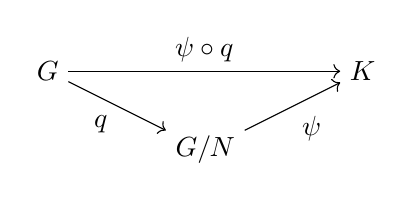
\begin{tikzpicture}
    \node (G) at (0, 1){$G$};
    \node (K) at (4, 1){$K$};
    \node (GN) at (2, 0){$G/N$};
    \draw[->] (G)--(K) node[midway, above]{$\psi \circ q$};
    \draw[->] (G)--(GN) node[midway, below left]{$q$};
    \draw[->] (GN)--(K) node[midway, below right]{$\psi$};
  \end{tikzpicture}
\end{center}

Every such $\psi$ gives a homomorphism $\psi \circ q \colon G \to K$ (called the \hldef{lift} or
\hldef{pullback} of $\psi$).
What homomorphisms $G \to K$ do we get?

\begin{center}
  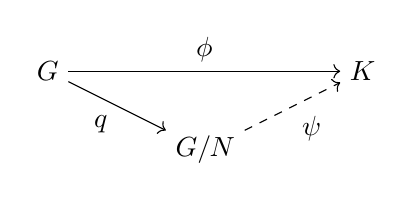
\begin{tikzpicture}
    \node (G) at (0, 1){$G$};
    \node (K) at (4, 1){$K$};
    \node (GN) at (2, 0){$G/N$};
    \draw[->] (G)--(K) node[midway, above]{$\phi$};
    \draw[->] (G)--(GN) node[midway, below left]{$q$};
    \draw[->, dashed] (GN)--(K) node[midway, below right]{$\psi$};
  \end{tikzpicture}
\end{center}

Given $\phi$, when can we fill in $\psi$ so that the diagram \hldef{commutes} (the paths are
equivalent)?

\begin{thm}{Universal property of quotients}{}
  Suppose $\phi \colon G \to K$ is a homomorphism and $N \trianglelefteq G$.
  Let $q \colon G \to G/N$ be the quotient homomorphism.
  Then there is a homomorphism $\psi \colon G/N \to K$ such that $\psi \circ q = \phi$ if and only
  if $N \subseteq \ker\phi$.
  Furthermore, if $\psi$ exists then it is unique.
\end{thm}

In other words, we can fill in $\psi$ if and only if $N \subseteq \ker\phi$.

\begin{defn}{set of morphisms}{}
  If $G, K$ are groups, let $\Hom(G, K)$ be the set of morphisms $G \to K$.
\end{defn}

\begin{cor}{}{}
  For any groups $G, K$ and $N \trianglelefteq G$, the function
  \[
    q^* \colon \Hom(G/N, K) \to \{\phi \in \Hom(G, K) : N \subseteq \ker\phi\}
      : \psi \mapsto \psi \circ q
  \]
  is a bijection.
\end{cor}

\pagebreak
\subsection{Comparison to universal property of products}

From before (but without the name):
\begin{thm}{Universal property of products}{}
  Let $\alpha \colon H \to G$ and $\beta \colon K \to G$ be homomorphisms, and let
  $i_H \colon H \to H \times K$ and $i_K \colon K \to H \times K$ be the inclusions of $H$ and $K$
  in $H \times K$.
  Then there is a homomorphism $\phi \colon H \times K \to G$ such that $\phi \circ i_H = \alpha$
  and $\phi \circ i_K = \beta$ if and only if $\alpha(h)\beta(k) = \beta(k)\alpha(h)$ for all
  $h \in H$ and $k \in K$.
\end{thm}

\begin{center}
  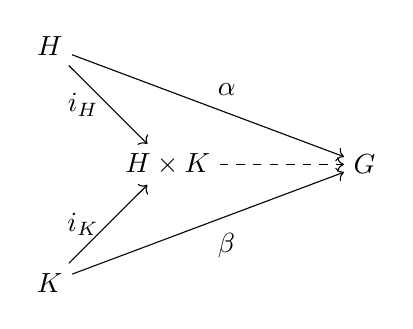
\begin{tikzpicture}
    \node (H) at (0, 1.5){$H$};
    \node (K) at (0, -1.5){$K$};
    \node (HK) at (1.5, 0){$H \times K$};
    \node (G) at (4, 0){$G$};
    \draw[->] (H)--(HK) node[midway, left]{$i_H$};
    \draw[->] (K)--(HK) node[midway, left]{$i_K$};
    \draw[->] (H)--(G) node[midway, above right]{$\alpha$};
    \draw[->] (K)--(G) node[midway, below right]{$\beta$};
    \draw[->, dashed] (HK)--(G);
  \end{tikzpicture}
\end{center}

\begin{cor}{}{}
  There is a bijection between $\Hom(H \times K, G)$ and
  $\{(\alpha, \beta) \in \Hom(H, G) \times \Hom(K, G) : \alpha(h)\beta(k) = \beta(k)\alpha(h)
    \text{ for all } h \in H \text{ and } k \in K\}$.
\end{cor}

We need some more machinery to justify why these are ``universal properties'', but for now we can
think of them as setting up important bijections.

\pagebreak
\subsection{Proving the universal property of quotients}

\begin{lem}{}{}
  If $\alpha \colon G \to H$ is surjective and $\psi_1, \psi_2 : H \to K$ are such that
  $\psi_1 \circ \alpha = \psi_2 \circ \alpha$, then $\psi_1 = \psi_2$.
\end{lem}

\begin{thmproof}
  If $h \in H$, then there is $g \in G$ with $\alpha(g) = h$.
  So $\psi_1(h) = \psi_1(\alpha(g)) = \psi_2(\alpha(g)) = \psi_2(h)$.
\end{thmproof}

Restatement for reference:

\begin{thm}{Universal property of quotients}{}
  Suppose $\phi \colon G \to K$ is a homomorphism and $N \trianglelefteq G$.
  Let $q \colon G \to G/N$ be the quotient homomorphism.
  Then there is a homomorphism $\psi \colon G/N \to K$ such that $\psi \circ q = \phi$ if and only
  if $N \subseteq \ker\phi$.
  Furthermore, if $\psi$ exists then it is unique.
\end{thm}

\begin{thmproof}
  If $\psi$ exists and $n \in N$, then $\phi(n) = \psi(q(n)) = \psi(e) = e$ so
  $N \subseteq \ker\phi$.

  Suppose $N \subseteq \ker\phi$.
  Define $\psi \colon G/N \to K : [g] \mapsto \phi(g)$.
  To show $\psi$ is well-defined, note that if $[g] = [h]$ then $g^{-1}h \in N \subseteq \ker\phi$,
  so $\phi(g^{-1})\phi(h) = \phi(g^{-1}h) = e$, so $\phi(g) = \phi(h)$.

  Clearly $\psi \circ q(g) = \psi([g]) = \phi(g)$ for all $g \in G$, so $\psi \circ q = \phi$.

  If $[g], [h] \in G/N$, then
  \[
    \psi([g] \cdot [h]) = \psi([gh]) = \phi(gh) = \phi(g)\phi(h) = \psi([g])\psi([h])
  \]
  so $\psi$ is a homomorphism.

  If $\psi' \colon G/N \to K$ is another homomorphism with $\psi' \circ q = \phi$, then
  $\psi' \circ q = \psi \circ q$ which implies $\psi' = \psi$ by the lemma ($q$ is surjective).
  So uniqueness holds.
\end{thmproof}

Note $\phi(gN) = \phi(g)\phi(N) = \phi(g)\{e\} = \{\phi(g)\}$.
So if $S \in G/N$, then $\phi(S) = \{b\}$, a singleton set.
Thus an equivalent way of defining $\psi$ is by $\psi(S) = b$ for $b \in K$ such that
$\phi(S) = \{b\}$.

\pagebreak
\subsection{The first isomorphism theorem}

Recall: if $\phi \colon G \to K$ is a homomorphism then $[G : \ker\phi] = \abs{\Im\phi}$.

Proof: there is a bijection $\psi \colon G/\ker\phi \to \Im\phi$ defined by $\psi(S) = b$ where
$b \in K$ is such that $\phi(S) = \{b\}$.

This looks like what we just did!

Now we also know $G/\ker\phi$ is a group, so $\abs{G/\ker\phi} = [G : \ker\phi] = \abs{\Im\phi}$.
Maybe this bijection is an isomorphism?

\begin{thm}{First isomorphism theorem}{}
  Suppose that $\phi \colon G \to K$ is a homomorphism.
  Then there is an isomorphism $\psi \colon G/\ker\phi \to \Im\phi$ such that $\phi = \psi \circ q$,
  where $q \colon G \to G/\ker\phi$ is the quotient homomorphism.
\end{thm}

\begin{thmproof}
  First, $\ker\phi \subseteq \ker\phi$, so by the universal property there is a homomorphism
  $\psi \colon G/\ker\phi \to K$ with $\psi \circ q = \phi$.

  Next $\psi([g]) = \phi(g)$ so clearly $\Im\psi = \Im\phi$.
  Thus we can regard $\psi$ as a surjective homomorphism $G/\ker\phi \to \Im\phi$.

  To see $\psi$ is a bijection, note $\psi$ agrees with the function $G/\ker\phi \to \Im\phi$
  defined previous to the theorem.

  Alternatively, notice if $\psi([g]) = e$, then $\phi(g) = e$, so $g \in \ker\phi$ and thus
  $[g] = [e]$.
  Then $\psi$ is injective by proposition.
\end{thmproof}

\begin{ex}
  The first isomorphism theorem is usually the best way to determine $G/N$:
  \begin{itemize}
    \item
    Recall $\SL_n\mathbb{K} \trianglelefteq \GL_n\mathbb{K}$ is defined as the kernel of the
    determinant homomorphism $\det \colon \GL_n\mathbb{K} \to \mathbb{K}^\times$.
    The image is $\Im\det = \mathbb{K}^\times$.

    By first isomorphism theorem, $\GL_n\mathbb{K} / \SL_n\mathbb{K} \cong \mathbb{K}^\times$.
    (Here, we only use the existence of $\psi$.)
    \item
    Consider $\Z \trianglelefteq \R^+$.
    What is $\R/\Z$?

    We have a homomorphism $\exp \colon \R \to \C^\times : x \mapsto e^{2\pi ix}$
    and we know $e^{2\pi ix} = 1$ if and only if $x \in \Z$ (so $\ker\exp = \Z$).
    Then $\Im\exp = \{a \in \C : \abs{a} = 1\} =: S^1$ (the \hldef{circle group}).

    So $\R/\Z \cong S^1$.
  \end{itemize}
\end{ex}

In general, to find $G/N$ we can try finding a group $K$ and homomorphism $\phi \colon G \to K$
where $\ker\phi = N$.
Then the first isomorphism theorem yields $G/N \cong \Im\phi$.

There are several more examples on the homework.

Sometimes, we can also turn this around and use the first isomorphism theorem to find $\Im\phi$.

\pagebreak
\subsection{Images and pullbacks}

We want to understand subgroups of $G/N$ using $q \colon G \to G/N$.

Recall: if $f \colon X \to Y$ is a function and $S \subseteq X$ and $T \subseteq Y$, then
\begin{itemize}
  \item $f(S) := \{f(x) : x \in S\}$ and
  \item $f^{-1}(T) := \{x \in X : f(x) \in T\}$.
\end{itemize}

From week 2:

\begin{prop}{}{}
  If $\phi \colon G \to H$ is a homomorphism and $K \leq G$, then $\phi(K) \leq H$.
\end{prop}

The ``pushforward'' or image of a subgroup is a subgroup.

\begin{prop}{}{}
  If $\phi \colon G \to H$ is a homomorphism and $K \leq H$, then $\phi^{-1}(K) \leq G$.
\end{prop}

The pullback of a subgroup is a subgroup.

\pagebreak
\subsection{Subgroup correspondence for isomorphisms}

If $f \colon X \to Y$ is a bijection, then $f^{-1}(f(S)) = S$ and $f(f^{-1}(T)) = T$.
Thus if $\phi \colon G \to H$ is an isomorphism, we get a bijection
\begin{center}
  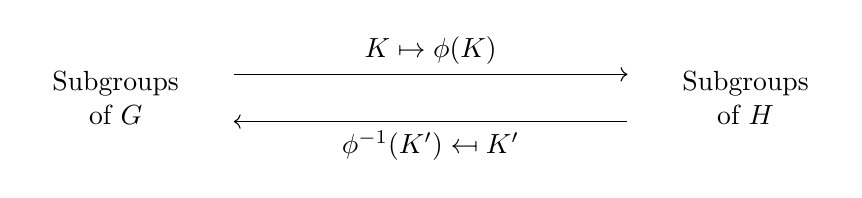
\begin{tikzpicture}
    \node[align=center, text width=2cm] at (0, 0){Subgroups of $G$};
    \node[align=center, text width=2cm] at (8, 0){Subgroups of $H$};
    \draw[->] (1.5, 0.3)--(6.5, 0.3) node[midway, above]{$K \mapsto \phi(K)$};
    \draw[->] (6.5, -0.3)--(1.5, -0.3) node[midway, below]{$\phi^{-1}(K') \mapsfrom K'$};
  \end{tikzpicture}
\end{center}

Furthermore:
\begin{itemize}
  \item $K_1 \leq K_2 \iff \phi(K_1) \leq \phi(K_2)$
  \item $\phi(K_1 \cap K_2) = \phi(K_1) \cap \phi(K_2)$
  \item $K$ is normal $\iff$ $\phi(K)$ is normal
  \item $\phi(\ang{S}) = \ang{\phi(S)}$
  \item $[G : K] = [H : \phi(K)]$
\end{itemize}

\pagebreak
\subsection{Set operation identities}

Some identities for bijections don't hold for general functions.

\begin{center}
  \renewcommand{\arraystretch}{1.5}
  \begin{tabular}{ll}
    Always hold                                            & Don't always hold \\
    \hline
    $A \subseteq B \implies f(A) \subseteq f(B)$           & $f(A \cap B) = f(A) \cap f(B)$ \\
    $A \subseteq B \implies f^{-1}(A) \subseteq f^{-1}(B) \qquad$ & $f^{-1}(f(A)) = A$ \\
    $f^{-1}(A \cup B) = f^{-1}(A) \cup f^{-1}(B)$          & $f(f^{-1}(B)) = B$ \\
    $f^{-1}(A \cap B) = f^{-1}(A) \cap f^{-1}(B)$          & \\
    $f(A \cup B) = f(A) \cup f(B)$                         & \\
  \end{tabular}
\end{center}

The left column holds for all functions; the right column holds for bijections but not for general
functions.

One consequence of these identities is that order is preserved:

\begin{lem}{}{}
  If $\phi \colon G \to H$ is a homomorphism, then:
  \begin{enumerate}
    \item If $K_1 \leq K_2 \leq G$, then $f(K_1) \leq f(K_2)$.
    \item If $K_1 \leq K_2 \leq H$, then $f^{-1}(K_1) \leq f^{-1}(K_2)$.
  \end{enumerate}
\end{lem}

Note we can't say that $K_1 \leq K_2 \iff \phi(K_1) \leq \phi(K_2)$ since
$\phi^{-1}(\phi(K)) \neq K$ in general.

Another consequence is that pullbacks preserve intersection:

\begin{lem}{}{}
  If $\phi \colon G \to H$ is a homomorphism and $K_1, K_2 \leq H$, then
  $\phi^{-1}(K_1 \cap K_2) = \phi^{-1}(K_1) \cap \phi^{-1}(K_2)$.
\end{lem}

\pagebreak
\subsection{Set operation identities for surjections}

If we suppose $f \colon X \to Y$ is surjective, the table changes:

\begin{center}
  \renewcommand{\arraystretch}{1.5}
  \begin{tabular}{ll}
    Always hold                                            & Don't always hold \\
    \hline
    $A \subseteq B \implies f(A) \subseteq f(B)$           & $f(A \cap B) = f(A) \cap f(B)$ \\
    $A \subseteq B \implies f^{-1}(A) \subseteq f^{-1}(B) \qquad$ & $f^{-1}(f(A)) = A$ \\
    $f^{-1}(A \cup B) = f^{-1}(A) \cup f^{-1}(B)$          & \sout{$f(f^{-1}(B)) = B$} \\
    $f^{-1}(A \cap B) = f^{-1}(A) \cap f^{-1}(B)$          & \\
    $f(A \cup B) = f(A) \cup f(B)$                         & \\
    $f(f^{-1}(B)) = B$                                     & \\
  \end{tabular}
\end{center}

\begin{lem}{}{}
  If $\phi \colon G \to H$ is a surjective homomorphism and $K \leq H$, then
  $\phi(\phi^{-1}(K)) = K$.
\end{lem}

\begin{defn}{set of subgroups}{}
  If $G$ is a group, let $\Sub(G)$ denote the set of subgroups of $G$.
\end{defn}

If $\phi \colon G \to H$ is a homomorphism, we get the induced functions
$\phi \colon \Sub(G) \to \Sub(H)$ and $\phi^{-1} \colon \Sub(H) \to \Sub(G)$.

If $\phi$ is surjective, the lemma shows $\phi$ is a left inverse to $\phi^{-1}$.
So $\phi^{-1} \colon \Sub(H) \to \Sub(G)$ is injective (from homework 1).

Question: what's the image of $\phi^{-1}$ in $\Sub(G)$?

\pagebreak
\subsection[The set of pullbacks in Sub(G)]{The set of pullbacks in $\Sub(G)$}

\begin{lem}{}{}
  Let $\phi \colon G \to H$ be a homomorphism.
  Then:
  \begin{enumerate}
    \item If $K \leq H$, then $\ker\phi \leq \phi^{-1}(K)$.
    \item If $\ker\phi \leq K \leq G$, then $\phi^{-1}(\phi(K)) = K$.
  \end{enumerate}
\end{lem}

\begin{thmproof}
  \begin{enumerate}
    \item $\ker\phi = \phi^{-1}(\{e\}) \subseteq \phi(H)$.
    \item $K \leq \phi^{-1}(\phi(K))$ is easy.
    Suppose $y \in \phi^{-1}(\phi(K))$.
    Then $\phi(y) \in \phi(K)$, so $\phi(y) = \phi(k)$ for some $k \in K$.
    Since $\phi(k^{-1}y) = e$, we get $k^{-1}y \in \ker\phi \subseteq K \implies y \in K$.
    We conclude that $\phi^{-1}(\phi(K)) \subseteq K$.
  \end{enumerate}
\end{thmproof}

Conclusion: $K = \phi^{-1}(K') \iff \ker\phi \leq K$ ($K$ is a pullback iff $K$ contains the
kernel).

\begin{thm}{Correspondence theorem}{}
  Let $\phi \colon G \to H$ be a surjective homomorphism.
  Then there is a bijection
  \begin{center}
    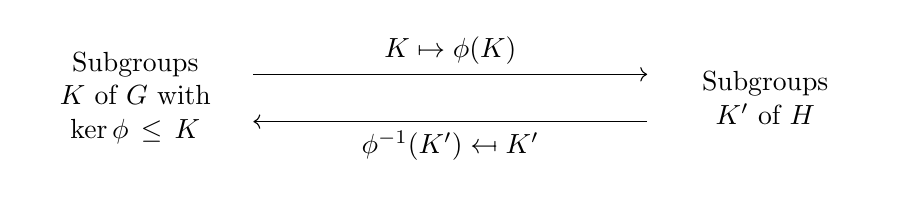
\begin{tikzpicture}
      \node[align=center, text width=2.5cm] at (0, 0){Subgroups $K$ of $G$ with $\ker\phi \leq K$};
      \node[align=center, text width=2.5cm] at (8, 0){Subgroups $K'$ of $H$};
      \draw[->] (1.5, 0.3)--(6.5, 0.3) node[midway, above]{$K \mapsto \phi(K)$};
      \draw[->] (6.5, -0.3)--(1.5, -0.3) node[midway, below]{$\phi^{-1}(K') \mapsfrom K'$};
    \end{tikzpicture}
  \end{center}
  Furthermore, if $\ker\phi \leq K, K_1, K_2 \leq G$ then
  \begin{enumerate}
    \item $K_1 \leq K_2 \iff \phi(K_1) \leq \phi(K_2)$,
    \item $\phi(K_1 \cap K_2) = \phi(K_1) \cap \phi(K_2)$, and
    \item $K$ is normal $\iff$ $\phi(K)$ is normal.
  \end{enumerate}
\end{thm}

\begin{thmproof}
  Since $\phi$ is surjective, $\phi(\phi^{-1}(K')) = K'$ for all $K' \leq H$.
  Conversely, if $\ker\phi \leq K \leq G$ then $\phi^{-1}(\phi(K)) = K$.
  So $\phi$ and $\phi^{-1}$ are inverses on the specified sets.

  \begin{enumerate}
    \item Follows from the fact that $\phi$ and $\phi^{-1}$ are inverses and preserve $\leq$.
    \item By lemma, $\phi^{-1}(\phi(K_1) \cap \phi(K_2))
      = \phi^{-1}(\phi(K_1)) \cap \phi^{-1}(\phi(K_2)) = K_1 \cap K_2$.
      Applying $\phi$ to both sides, we see also $\phi(K_1 \cap K_2) = \phi(K_1) \cap \phi(K_2)$.
    \item (Homework.)
  \end{enumerate}
\end{thmproof}

\pagebreak
\subsection{Correspondence theorem for quotient groups}

If $N \trianglelefteq G$, then $q \colon G \to G/N$ is a surjection.

\begin{thm}{Correspondence theorem for quotient groups}{}
  Let $N \trianglelefteq G$.
  Then there is a bijection
  \begin{center}
    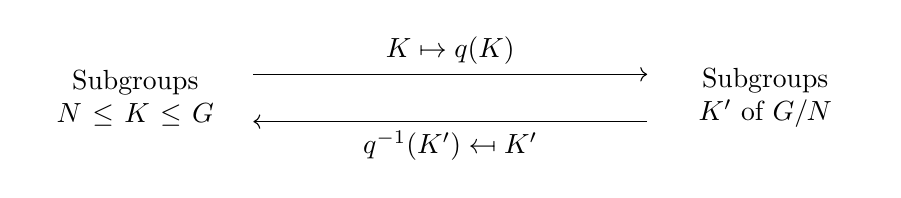
\begin{tikzpicture}
      \node[align=center, text width=2.5cm] at (0, 0){Subgroups $N \leq K \leq G$};
      \node[align=center, text width=2.5cm] at (8, 0){Subgroups $K'$ of $G/N$};
      \draw[->] (1.5, 0.3)--(6.5, 0.3) node[midway, above]{$K \mapsto q(K)$};
      \draw[->] (6.5, -0.3)--(1.5, -0.3) node[midway, below]{$q^{-1}(K') \mapsfrom K'$};
    \end{tikzpicture}
  \end{center}
  Furthermore, if $N \leq K, K_1, K_2 \leq G$ then
  \begin{enumerate}
    \item $K_1 \leq K_2 \iff q(K_1) \leq q(K_2)$,
    \item $q(K_1 \cap K_2) = q(K_1) \cap q(K_2)$, and
    \item $K$ is normal $\iff$ $q(K)$ is normal.
  \end{enumerate}
\end{thm}

This seems like a specialization of the correspondence theorem, but they are actually equivalent
(with some work).

Recall the first isomorphism theorem tells us that if $\phi \colon G \to H$ is a surjective
homomorphism, then $G/\ker\phi \cong H$.
So there is a bijection between $\Sub(H)$ and $\Sub(G/\ker\phi)$.

As an exercise, check that (first isomorphism theorem) + (subgroup correspondence for isomorphisms)
+ (correspondence theorem for quotient groups) implies (correspondence theorem for surjective
homomorphisms).

\pagebreak
\subsection[Identifying q(K)]{Identifying $q(K)$}

Suppose $N \trianglelefteq G$ and $N \leq K \leq G$.
Let $q_G \colon G \to G/N$ be the quotient map.
Since $N \trianglelefteq K$, we also have the quotient map $q_K \colon K \to K/N$.

\begin{center}
  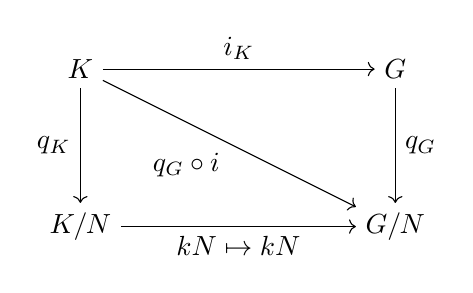
\begin{tikzpicture}
    \node (K) at (0, 2){$K$};
    \node (KN) at (0, 0){$K/N$};
    \node (G) at (4, 2){$G$};
    \node (GN) at (4, 0){$G/N$};
    \draw[->] (K)--(KN) node[midway, left]{$q_K$};
    \draw[->] (K)--(G) node[midway, above]{$i_K$};
    \draw[->] (K)--(GN) node[midway, below left]{$q_G \circ i$};
    \draw[->] (G)--(GN) node[midway, right]{$q_G$};
    \draw[->] (KN)--(GN) node[midway, below]{$kN \mapsto kN$};
  \end{tikzpicture}
\end{center}

Since $\ker q_G \circ i = N$, the first isomorphism theorem tells us there is an isomorphism
$\psi \colon K/N \to \Im q \circ i_K = q(K)$ such that $\psi \circ q_K = q_G \circ i$.

In other words, if $k \in K$ then $\psi(kN) = q(k) = kN$.

\begin{prop}{}{}
  Suppose $N \trianglelefteq G$ and $N \leq K \leq G$.
  Let $q \colon G \to G/N$ be the quotient map.

  Then the function $K/N \to q(K) \leq G/N \colon kN \mapsto kN$ is an isomorphism.
\end{prop}

Because of this isomorphism, we use the following notation:

\begin{defn}{subgroup $q(K)$}{}
  If $N \trianglelefteq G$ and $N \leq K \leq G$, then the subgroup $q(K)$ corresponding to $K$ in
  $G/N$ is denoted by $K/N$.
\end{defn}

\begin{ex}
  \begin{itemize}
    \item Let $G = D_{2n}$ and $N = \ang{s}$ where $s$ is the rotation generator.

    Subgroups of $D_{2n}$ containing $N$ correspond to subgroups of $D_{2n}/N = \Zmod{2}$.
    $\Zmod{2}$ only has two subgroups, itself and $\{e\}$.
    So there are only two subgroups of $D_{2n}$ containing $N$.
    \item
    $\GL_n\mathbb{K}/\SL_n\mathbb{K} \cong \mathbb{K}^\times$, so subgroups of $\GL_n\mathbb{K}$
    containing $\SL_n\mathbb{K}$ correspond to subgroups of $\mathbb{K}^\times$ (of which there
    can be many).
  \end{itemize}
\end{ex}

%%%%% Lec 11
\section{Second and third isomorphism theorems}

\subsection{Third isomorphism theorem}

What about quotients of quotients?

Suppose $N \trianglelefteq G$ and $N \leq K \leq G$.

From the correspondence theorem (homework), $K \trianglelefteq G$ if and only if
$K/N \trianglelefteq G/N$.
Then suppose $K/N \trianglelefteq G/N$.
What is $(G/N)/(K/N)$?

\begin{thm}{Third isomorphism theorem (informal version)}{}
  $(G/N)/(K/N) \cong G/K$.
\end{thm}

\begin{ex}
  Suppose $n \mid m$, so $m\Z \leq n\Z$ (and both are normal).

  Then $(\Z/m\Z)/(n\Z/m\Z) \cong \Z/n\Z$.
  For example, $(\Z/20\Z)/(5\Z/20\Z) \cong \Z/5\Z$.
\end{ex}

\begin{thm}{Third isomorphism theorem}{}
  Let $N \trianglelefteq G$ and $N \leq K \trianglelefteq G$.
  Let
  \begin{itemize}
    \item $q_1$ be the quotient map $G \to G/N$,
    \item $q_2$ be the quotient map $G/N \to (G/N)/(K/N)$, and
    \item $q_3$ be the quotient map $G \to G/K$.
  \end{itemize}
  Then there is an isomorphism $\psi \colon G/K \to (G/N)/(K/N)$ such that
  $\psi \circ q_3 = q_2 \circ q_1$.
\end{thm}

\begin{center}
  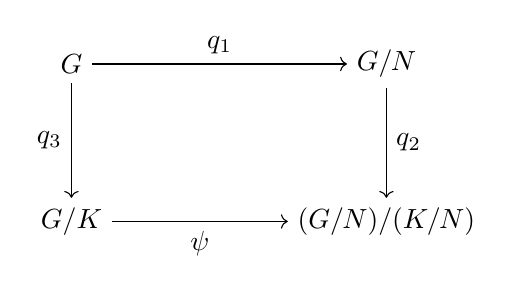
\begin{tikzpicture}
    \node (G) at (0, 2){$G$};
    \node (GN) at (4, 2){$G/N$};
    \node (GK) at (0, 0){$G/K$};
    \node (GNKN) at (4, 0){$(G/N)/(K/N)$};
    \draw[->] (G)--(GK) node[midway, left]{$q_3$};
    \draw[->] (G)--(GN) node[midway, above]{$q_1$};
    \draw[->] (GN)--(GNKN) node[midway, right]{$q_2$};
    \draw[->] (GK)--(GNKN) node[midway, below]{$\psi$};
  \end{tikzpicture}
\end{center}

\begin{thmproof}
  Note that $\ker q_2 \circ q_1 = (q_2 \circ q_1)^{-1}(\{e\}) = q_1^{-1}(q_2^{-1}(\{e\}))
    = q_1^{-1}(K/N) = K$.

  Since $q_2$ and $q_1$ are surjective, $\Im q_2 \circ q_1 = (G/N)/(K/N)$.

  By the first isomorphism theorem, there is an isomorphism $\psi \colon G/K \to (G/N)/(K/N)$ such
  that $\psi \circ q_3 = q_2 \circ q_1$.
\end{thmproof}

\pagebreak
\subsection[What if K isn't normal?]{What if $K$ isn't normal?}

Then $G/K$ isn't a group, and neither is $(G/N)/(K/N)$.

However, we can still talk about $[G : K]$ and $[G/N : K/N]$.

\begin{prop}{}{}
  If $N \trianglelefteq G$ and $N \leq K \leq G$, then $[G : K] = [G/N : K/N]$.
\end{prop}

In fact, this doesn't even need quotient spaces.
This holds for surjective homomorphisms.

\begin{prop}{}{}
  Let $\phi \colon G \to H$ be a surjective homomorphism and suppose $\ker\phi \leq K \leq G$.
  Then $[G : K] = [H : \phi(K)]$.
\end{prop}

These are equivalent by the first isomorphism theorem.

\begin{thmproof}
  Define a function $f \colon G/K \to H/\phi(K) : gK \mapsto \phi(g)\phi(K)$.

  Well-defined: if $gK = hK$, then
  $h^{-1}g \in K \implies \phi(h)^{-1}\phi(g) = \phi(h^{-1}g) \in \phi(K)$.
  So $\phi(g)\phi(K) = \phi(h)\phi(K)$.

  Since $\phi$ is surjective, $f$ is surjective.

  Suppose $f(gK) = f(hK)$ so $\phi(g)\phi(K) = \phi(h)\phi(K)$.
  Then $\phi(h^{-1}g) = \phi(h)^{-1}\phi(g) \in \phi(K)$ which shows
  $h^{-1}g \in \phi^{-1}(\phi(K)) = K$ by the correspondence theorem.
  So $gK = hK$ and $f$ is injective.

  Then $f$ is a bijection, so the indices must be equal.
\end{thmproof}

\pagebreak
\subsection{Revisiting products}

Recall this lemma:

\begin{lem}{}{}
  Suppose $G = HK$ for $H, K \leq G$ for $H, K \leq G$.
  Then every element $g \in G$ can be written as $g = hk$ for unique $h \in H$ and $k \in K$ if and
  only if $H \cap K = \{e\}$.
\end{lem}

Which motivated this definition:

\begin{defn}{internal direct product}{}
  $G$ is the \hldef{internal direct product} of subgroups $H, K \leq G$ if
  \begin{enumerate}
    \item $HK = G$,
    \item $H \cap K = \{e\}$, and
    \item $hk = kh$ for all $h \in H$ and $k \in K$.
  \end{enumerate}
\end{defn}

But the proof of the lemma did not use the fact that $G = HK$, so we can generalize it.

\begin{lem}{}{}
  Suppose $H, K \leq G$.
  Then every element of $HK$ can be written as $hk$ for unique $h \in H$ and $k \in K$ if and only
  if $H \cap K = \{e\}$.
\end{lem}

If $H \cap K = \{e\}$, then $\abs{HK} = \abs{H} \cdot \abs{K}$.

What if $H \cap K \neq \{e\}$?
Here, $HK = \bigcup_{h \in H} hK$, a union of cosets of $K$.
Let $X = \{hK : h \in H\} \subseteq G/K$.
Then $X$ is a partition of $HK$, so $\abs{HK} = \abs{X} \cdot \abs{K}$.
But how large is $X$?

\begin{lem}{}{}
  Let $H, K \leq G$.
  If $h_1, h_2 \in H$, then $h_1K = h_2K$ if and only if $h_1(H \cap K) = h_2(H \cap K)$.
\end{lem}

\begin{thmproof}
  $h_1K = h_2K \iff h_1^{-1}h_2 \in K \iff h_1^{-1}h_2 \in H \cap K$.
  But $h_1^{-1}h_2 \in H \cap K$ if and only if $h_1(H \cap K) = h_2(H \cap K)$.
\end{thmproof}

Rephrasing, consider the equivalence relations $\sim_K$ on $G$ and $\sim_{H \cap K}$ on $H$:
if $h_1, h_2\ in H$, then $h_1 \sim_K h_2 \iff h_1 \sim_{H \cap K} h_2$.

\begin{cor}{}{}
  $H/(H \cap K) \to X \colon h(H \cap K) \to hK$ is a bijection.
\end{cor}

\begin{thmproof}
  By the lemma, this is well-defined and injective.
  Surjectivity is obvious.
\end{thmproof}

Now we see $\abs{X} = [H : H \cap K]$, so $\abs{HK} = [H : H \cap K] \abs{K}$.
Lagrange's theorem yields $[H : H \cap K] \cdot \abs{H \cap K} = \abs{H}$, so we have:

\begin{prop}{}{}
  If $H, K \leq G$, then $\abs{HK}\abs{H \cap K} = \abs{H}\abs{K}$.
\end{prop}

If $H$ and $K$ are finite, another way to think of this formula is
$[H : H \cap K] = \abs{X} = \frac{\abs{HK}}{\abs{K}}$.

Is the fraction an index as well?
Maybe--$HK$ is not necessarily a group.

\begin{prop}{}{}
  Let $H, K \leq G$.
  Then $HK \leq G \iff HK = KH \iff KH \subseteq HK$.
\end{prop}

\begin{thmproof}
  If $HK \leq G$ and $h \in H$ and $k \in K$, then $h, k \in HK$ so $kh \in HK$.
  Also, $k^{-1}h^{-1} \in HK$, so $k^{-1}h^{-1} = h_0k_0$.
  Hence $hk = (k^{-1}h^{-1})^{-1} = k_0^{-1}h_0^{-1} \in KH$.
  So $KH \subseteq HK$ and $HK \subseteq KH$, hence $HK = KH$.

  Now suppose $KH \subseteq HK$, we need to show $HK \leq G$.
  We always have $e \in HK$.
  If $x, y \in HK$, then $x = h_0k_0$ and $y = h_1k_1$ for some $h_0, h_1 \in H$ and
  $k_0, k_1 \in K$.
  Since $KH \subseteq HK$, $k_0^{-1}h_0^{-1}h_1 = h_2k_2$ for some $h_2 \in H$ and $k_2 \in K$.
  So $x^{-1}y = k_0^{-1}h_0^{-1}h_1k_1 = h_2k_2k_1 \in HK$.
\end{thmproof}

Corollary: if $KH \subseteq HK$, then $[H : H \cap K] = [HK : K]$ (exercise: even for infinite
$HK$ or $K$).

When is $KH \subseteq HK$?

A sufficient condition is that for all $h \in H$, there is $h' \in H$ such that $Kh = h'K$.
Recall that if $Kh = h'K$, then $h'K = Kh$.
So we can rephrase this condition as $hKh^{-1} = K$ for all $h \in H$, or $H \subseteq N_G(K)$.

\begin{cor}{}{}
  If $H \subseteq N_G(K)$, then $HK \leq G$, and hence $[H : H \cap K] = [HK : K]$.
\end{cor}

What else does $H \subseteq N_G(K)$ imply?

We know $hKh^{-1} = K$ and $kKk^{-1} = K$, so
$H, K \subseteq N_{HK}(K) \implies N_{HK}(K) = HK \implies K \trianglelefteq HK$.

If $k \in H \cap K$ and $h \in H$, then $hkh^{-1} \in H \cap K$.
So $H \cap K \trianglelefteq H$.

\pagebreak
\subsection{Second isomorphism theorem}

\begin{thm}{Second isomorphism theorem}{}
  Suppose $H \subseteq N_G(K)$.
  Then $HK \leq G$, $K \trianglelefteq HK$, and $H \cap K \trianglelefteq H$.
  Furthermore, if $i_H \colon H \to HK$ is the inclusion and $q_1 \colon H \to H/(H \cap K)$ and
  $q_2 \colon HK \to HK/K$ are the quotient maps, then there is an isomorphism
  $\psi \colon H/(H \cap K) \to HK/K$ such that $\psi \circ q_1 = q_2 \circ i_H$.
\end{thm}

\begin{center}
  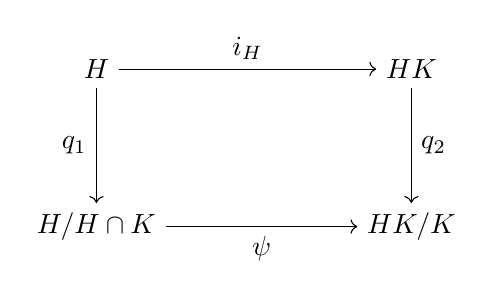
\begin{tikzpicture}
    \node (H) at (0, 2){$H$};
    \node (HK) at (4, 2){$HK$};
    \node (HHK) at (0, 0){$H/H \cap K$};
    \node (HKK) at (4, 0){$HK/K$};
    \draw[->] (H)--(HHK) node[midway, left]{$q_1$};
    \draw[->] (H)--(HK) node[midway, above]{$i_H$};
    \draw[->] (HK)--(HKK) node[midway, right]{$q_2$};
    \draw[->] (HHK)--(HKK) node[midway, below]{$\psi$};
  \end{tikzpicture}
\end{center}

\begin{thmproof}
  We've already shown $HK \leq G$, $K \trianglelefteq HK$, and $H \cap K \trianglelefteq H$.

  If $h \in H$ and $k \in K$, then $hkK = hK$.
  So $HK/K = \{gK : g \in HK\} = \{hK : h \in H\}$.
  Hence $\Im q_2 \circ i_H = \{hK : h \in H\} = HK/K$.

  Next, $\ker q_2 \circ i_H = i_H^{-1}(q_2^{-1}(\{e\})) = i_H^{-1}(K) = H \cap K$.

  By the first isomorphism theorem, there is an isomorphism $\psi$ as desired.
\end{thmproof}

\begin{ex}[Example: $\PGL_n\C$]
  Recall $\PGL_n\C = \GL_n\C / Z(\GL_n\C)$.

  Let $K = Z(\GL_n\C) = \{\lambda 1 : \lambda \neq 0\}$.

  Since $K \trianglelefteq \GL_n\C$, $N_{\GL_n\C}(K) = \GL_n\C$.

  Take $H = \SL_n\C = \{M \in \GL_n\C : \det M = 1\}
    \trianglelefteq \GL_n\C = N_{\GL_n\C}(K)$, so $HK \leq \GL_n\C$ by the
  second isomorphism theorem.

  Suppose $M \in \GL_n\C$ and let $\lambda = \det M$.
  Then $\det \lambda^{-1/n}M = \lambda^{-1} \det M = 1$, so $\lambda^{-1/n}M \in H$ (for any
  choice of $\lambda^{-1/n}$).

  We conclude $\GL_n\C = HK$.

  Now define $C_n := H \cap K = \{\lambda 1 : \lambda^n = 1\}
    = \{e^{2\pi i k/n} : k = 0, \ldots, n - 1\}$.
  (Note $C_n \cong \Zmod{n}$.)

  By the second isomorphism theorem, $\PGL_n\C \cong \SL_n\C/C_n$.
\end{ex}

\week{Group Actions}

%%%%% Lec 12
\section{Group actions and Cayley's theorem}

\subsection{Group actions}

\begin{ex}
  Permutations $S_n$ of $\{1, \ldots, n\}$ form a group.

  This means we can multiply permutations together: e.g. $(12)(34)(24) = (1234)$.

  But we can also plug in numbers from $\{1, \ldots, n\}$: e.g. $((12)(34))(3) = 4$.

  We say that $S_n$ \hldef{acts} on $\{1, \ldots, n\}$.
\end{ex}

\begin{ex}
  Similarly, for $\GL_n\C$, we can do more than multiply matrices: we can also multiply
  matrices and vectors.

  Given $A \in \GL_n\C$ and $v \in \C^n$, we get $Av \in \C^n$.

  We say that $\GL_n\C$ \hldef{acts} on $\C^n$.
\end{ex}

Group actions can reveal a lot about a group.

\begin{defn}{(left) action}{}
  Let $G$ be a group.
  A \hldef{(left) action} of $G$ on a set $X$ is a function $\cdot \colon G \times X \to X$ such
  that
  \begin{enumerate}
    \item $e \cdot x = x$ for all $x \in X$, and
    \item $g \cdot (h \cdot x) = (gh) \cdot x$ for all $g, h \in G$ and $x \in X$.
  \end{enumerate}
\end{defn}

\begin{ex}
  \begin{itemize}
    \item $S_n$ acts on $\{1, \ldots, n\}$ for $n \geq 1$ (proof: below).
    \item $\GL_n\mathbb{K}$ acts on $\mathbb{K}^n$ (proof: exercise).
    \item If $X$ is any set and $G$ is any group, we can define an action of $G$ on $x$ by
      $g \cdot x = x$ for all $g \in G$ and $x \in X$.
      This is the \hldef{trivial action} of $G$ on $X$.
      Proof: (1) clear; (2) $g \cdot (h \cdot x) = g \cdot x = x = (gh) \cdot x$.
  \end{itemize}
\end{ex}

\begin{prop}{}{}
  Let $X$ be a set.
  The group $S_X$ (of invertible functions $X \to X$ under composition $\circ$) acts on $X$
  via $f \cdot x = f(x)$.
\end{prop}

\begin{thmproof}
  The identity 1 in $S_X$ is the identity function, so $1 \cdot x = 1(x) = x$.
  If $f, g \in S_X$, then $(f \circ g)(x) = f(g(x)) = f \cdot (g \cdot x)$.
\end{thmproof}

Note: usually we use notation $f(x)$ rather than $f \cdot x$.
Also, recall $S_n = S_{\{1, \ldots, n\}}$.

\begin{lem}{}{}
  If $G$ acts on $X$ and $H \leq G$, then $H$ acts on $X$ by the restricted action
  $H \times X \to X : (h, x) \mapsto h \cdot x$.
\end{lem}

Hence an alternative way to show $\GL_n\mathbb{K}$ acts on $\mathbb{K}^n$ is to observe
$\GL_n\mathbb{K} \leq S_{\mathbb{K}^n}$.
(Invertible $n \times n$ matrices are invertible functions $\mathbb{K}^n \to \mathbb{K}^n$.)

\pagebreak
\subsection{Invariant subsets}

Groups aren't tied to a particular action.

\begin{ex}
  $D_{2n}$ was defined as a subgroup of $\GL_2\R$, so it acts on $\R^2$.

  However, $D_{2n}$ also acts on the vertices $v_0, \ldots, v_{n - 1}$ of the $n$-gon.

  In fact, this action determines elements of $D_{2n}$:
  \begin{itemize}
    \item $s^i$ sends $v_0 \mapsto v_i$ and $v_1 \mapsto v_{i + 1}$
    \item $s^i r$ sends $v_0 \mapsto v_i$ and $v_1 \mapsto v_{i - 1}$
  \end{itemize}
\end{ex}

This dihedral group action on the vertices of the $n$-gon is a special case of a pattern.

\begin{defn}{invariant under an action}{}
  If $G$ acts on $X$, a subset $Y \subseteq X$ is \hldef{invariant under the action of} $G$ if
  $g \cdot y \in Y$ for all $g \in G$ and $y \in Y$.
\end{defn}

\begin{lem}{}{}
  If $G$ acts on $X$ and $Y$ is an invariant subset, then $G$ acts on $Y$ via
  $G \times Y \to Y : (g, y) \mapsto g \cdot y$.
\end{lem}

\begin{ex}
  $\{0\}$ is an invariant subset of $\mathbb{K}^n$ under the action of $\GL_n\mathbb{K}$.
  In this case, the action of $\GL_n\mathbb{K}$ on $\{0\}$ is the trivial action.
\end{ex}

\pagebreak
\subsection{Actions on functions}

\begin{prop}{}{}
  Suppose $G$ acts on $X$ and $Y$, and let $\Fun(X, Y)$ denote the set of functions from $X$ to $Y$.

  If $g \in G$ and $f \in \Fun(X, Y)$, let $g \cdot f$ be the function
  \[ g \cdot f \colon X \to Y : x \mapsto g \cdot f(g^{-1} \cdot x). \]
  Then $G \times \Fun(X, Y) : (g, f) \mapsto g \cdot f$ is a left action of $G$ on $\Fun(X, Y)$.
\end{prop}

\begin{thmproof}[Proof (homework).]
\end{thmproof}

Often we apply this function with the trivial action on $Y$, so the action looks like
$g \cdot f(x) = f(g^{-1} \cdot x)$.

\pagebreak
\subsection{Actions on subsets}

\begin{prop}{}{}
  Suppose $G$ acts on $X$, and let $2^X$ denote the set of subsets of $X$.
  Then $g \cdot S = \{g \cdot s : s \in S\}$ defines an action of $G$ on $2^X$.
\end{prop}

\begin{thmproof}
  Let $S \in 2^X$.

  First, $e \cdot S = \{e \cdot s : s \in S\} = \{s : s \in S\} = S$.

  Next, let $g, h \in G$.
  Then
  \begin{align*}
    g \cdot (h \cdot S)
    &= g \cdot \{h \cdot s : s \in S\} \\
    &= \{g \cdot (h \cdot s) : s \in S\} \\
    &= \{gh \cdot s : s \in S\} \\
    &= gh \cdot S.
  \end{align*}
\end{thmproof}

Alternative proof: use $2^X$ as the set of functions $X \to \{0, 1\}$.
Realize action of $G$ on $2^X$ by taking action on functions with trivial action on $\{0, 1\}$
(homework).

\pagebreak
\subsection{Left regular actions}

Does every group act on some set?

\begin{lem}{}{}
  If $G$ is a group, then the multiplication map $\cdot \colon G \times G \to G$ is a left action
  of $G$ on $G$.
\end{lem}

\begin{thmproof}
  Immediate from group definition.
\end{thmproof}

So every group acts on itself by left multiplication.
This action is called the \hldef{left regular action} of $G$ on $G$.

\begin{lem}{}{}
  If $H \leq G$, then $G$ acts on $G/H$ by $g \cdot (kH) = gkH$.
\end{lem}

\begin{thmproof}
  $G/H$ is an invariant subset of $2^G$.
\end{thmproof}

Since $G/\{e\} = G$, this generalizes the left regular action.

\pagebreak
\subsection{Right actions}

\begin{ex}
  Let $G$ be a group where the product of $g$ and $h$ is denoted $gh$.

  For $g, k \in G$, define $g \cdot k = kg$ (right multiplication).
  If $g, h, k \in G$, then $g \cdot (h \cdot k) = g \cdot kh = khg$, but $gh \cdot k = kgh$, which
  is not equal to $kgh$ if $hg \neq gh$.

  So right multiplication does not define a left action in general.
\end{ex}

Can we fix this?

\begin{defn}{(right) action}{}
  Let $G$ be a group.
  A \hldef{(right) action} of $G$ on a set $X$ is a function $\cdot \colon X \times G \to X$ such
  that
  \begin{enumerate}
    \item $x \cdot e = x$ for all $x \in X$, and
    \item $(x \cdot g) \cdot h = x \cdot (gh)$ for all $g, h \in G$ and $x \in X$.
  \end{enumerate}
\end{defn}

\begin{ex}
  \begin{itemize}
    \item There is a right action of $G$ on itself by right multiplication.
    This is called the \hldef{right regular action} of $G$ on $G$.
    More generally, if $H \leq G$ then $G$ acts on $H \backslash G$.
    \item If $G$ is a group and $X$ is a set, then there is a trivial right action of $G$ on $X$
    defined by $x \cdot g = x$ for all $g \in G$ and $x \in X$.
    \item If there is a right action of $G$ on $X$, and $Y$ is any set, then
    $(g \cdot f)(x) = f(g \cdot x)$ defines a \emph{left} action of $G$ on $\Fun(X, Y)$.
  \end{itemize}
\end{ex}

Can we reconcile right and left actions somehow?

\begin{prop}{}{}
  If $\cdot$ is a right action of $G$ on $X$, then $g \cdot x = x \cdot g^{-1}$ defines a left
  action of $G$ on $X$.
\end{prop}

\begin{thmproof}
  First $e \cdot x = x \cdot e = x$, and for $g, h \in G$ and $x \in X$, we get
  \begin{align*}
    g \cdot (h \cdot x)
    &= g \cdot (x \cdot h^{-1}) \\
    &= (x \cdot h^{-1}) \cdot g^{-1} \\
    &= x \cdot h^{-1}g^{-1} \\
    &= x \cdot (gh)^{-1} \\
    &= gh \cdot x.
  \end{align*}
\end{thmproof}

Combined with the last example, this proposition explains why if $\cdot$ is a left action of $G$
on $X$, we can define a left action of $G$ on $\Fun(X, Y)$ by setting
$(g \cdot f)(x) = f(g^{-1} \cdot x)$.

\pagebreak
\subsection{Permutation representations}

\begin{lem}{}{}
  If $G$ has a left action on a set $X$, and $g \in G$, let $\ell_g \colon X \to X$ be defined by
  $\ell_g(x) = g \cdot x$.
  Then:
  \begin{enumerate}
    \item $\ell_g \circ \ell_h = \ell_{gh}$ for all $g, h \in G$.
    \item $\ell_e = 1$, the identity function.
    \item $\ell_g$ is a bijection for all $g \in G$.
  \end{enumerate}
\end{lem}

\begin{thmproof}
  \begin{enumerate}
    \item $\ell_g \circ \ell_h(x) = g \cdot (h \cdot x) = gh \cdot x = \ell_{gh}(x)$.
    \item $\ell_e(x) = e \cdot x = x$.
    \item $\ell_g \circ \ell_{g^{-1}} = \ell_e = 1 = \ell_{g^{-1}} \circ \ell_g$, so $\ell_g$ is
      invertible.
  \end{enumerate}
\end{thmproof}

\begin{cor}{}{}
  Every left action of $G$ on $X$ gives a homomorphism $\phi \colon G \to S_X : g \mapsto \ell_g$
  with $\phi(g)(x) = g \cdot x$.
\end{cor}

\begin{defn}{permutation representation}{}
  If $X$ is a set, a \hldef{permutation representation} of $G$ on $X$ is a homomorphism
  $\phi \colon G \to S_X$.
\end{defn}

If $\abs{X} = n$, then $S_X \cong S_n$.
So an action on a finite set $X$ with $\abs{X} = n$ gives a homomorphism to $S_n$.

Example: $D_{2n}$ acts on $n$ vertices of the $n$-gon, so there is a homomorphism $D_{2n} \to S_n$.

\pagebreak
\subsection{Permutation representations of the dihedral group}

Let $X = \{v_0, \ldots, v_{n - 1}\}$ be the vertices of the $n$-gon.
We identify $X$ with $\{1, \ldots, n\}$ by mapping $v_i \mapsto i + 1$ so we can write elements of
$S_X$ as elements of $S_n$.

Let $\phi \colon D_{2n} \to S_n$ be a permutation representation given by the action of $D_{2n}$ on
$X$.

What is $\phi(s)$?
We see $s \cdot v_0 = v_1$, $s \cdot v_1 = v_2$, $\ldots$, $s \cdot v_n = v_0$, so
$\phi(s) = (1 \ 2 \ 3 \ \cdots \ n)$.

What is $\phi(r)$?
We see $r \cdot v_0 = v_0$, $r \cdot v_1 = v_{n - 1}$, $r \cdot v_2 = v_{n - 2}$, and in general
$r \cdot v_i = v_{n - i}$, so
\[
  \phi(r) = \begin{cases}
    (2 \ n)(3 \ n - 1) \cdots (\frac{n + 1}{2} \ \frac{n + 3}{2}) \qquad & n \text { odd} \\
    (2 \ n)(3 \ n - 1) \cdots (\frac{n}{2} \ \frac{n}{2} + 2) \qquad & n \text { even} \\
  \end{cases}.
\]

In general, $\phi(s^i r^j) = \phi(s)^i \phi(r)^j$.

(Note a different choice of $r$ could have yielded a different representation.)

\begin{thm}{}{}
  \begin{enumerate}
    \item If $G$ acts on $X$, then there is a homomorphism $\phi \colon G \to S_X$ defined by
      $\phi(g)(x) = g \cdot x$.
    \item If $\phi \colon G \to S_X$ is a homomorphism, then $g \cdot x = \phi(g)(x)$ defines a
      group action of $G$ on $X$.
  \end{enumerate}
\end{thm}

In other words, group actions are equivalent to permutation representations.
Because of this theorem, we treat the two as interchangeable.

\begin{thmproof}
  \begin{enumerate}
    \item Already done.
    \item First, $e \cdot x = \phi(e)(x) = 1(x) = x$ for all $x \in X$.
    Next, if $g, h \in G$ and $x \in X$, then
    \[ g \cdot (h \cdot x) = \phi(g)(\phi(h)(x)) = (\phi(g) \circ \phi(h))(x) = \phi(gh)(x). \]
  \end{enumerate}
\end{thmproof}

\pagebreak
\subsection{Faithful actions}

\begin{defn}{kernel, faithful}{}
  Let $G$ act on a set $X$, and let $\phi \colon G \to S_X$ be the corresponding permutation
  representation.
  The \hldef{kernel} of the action is $\ker \phi$, and the action is \hldef{faithful} if
  $\ker\phi = \{e\}$.
\end{defn}

That is, an action is faithful if the corresponding permutation representation is injective.

\begin{lem}{}{}
  An action of $G$ on $X$ is faithful if and only if for every $g \in G$ with $g \neq e$, there is
  $x \in X$ such that $g \cdot x \neq x$.
\end{lem}

\begin{thmproof}
  $\ell_g \neq 1$ if and only if there is $x \in X$ such that $g \cdot x = \ell_g(x) \neq x$.
\end{thmproof}

\begin{ex}
  \begin{itemize}
    \item $S_X$ acts faithfully on $X$.
    \item If $A \cdot e_i = e_i$ for all $i = 1, \ldots, n$, then $A = 1$, so the action of
      $\GL_n\mathbb{K}$ on $\mathbb{K}^n$ is faithful.
    \item $D_{2n}$ acts faithfully on vertices on the $n$-gon (exercise).
    \item The trivial action is not faithful.
  \end{itemize}
\end{ex}

Does every group act faithfully on some set?

\begin{thm}{Cayley's theorem}{}
  The left regular action of $G$ on $G$ is faithful.

  Consequently, $G$ is isomorphic to a subgroup of $S_G$.
  In particular, if $\abs{G} = n < \infty$, then $G$ is isomorphic to a subgroup of $S_n$.
\end{thm}

\begin{thmproof}
  If $g \in G$ with $g \neq e$, then $g \cdot e = g \neq e$.
  So the left regular action is faithful.

  Hence the permutation representation $\phi \colon G \to S_G$ is injective, and thus $G$ is
  isomorphic to $\Im\phi \leq S_G$ (first isomorphism theorem).

  If $\abs{G} = n < \infty$, then $S_G \cong S_n$.
\end{thmproof}

The homomorphism $G \to S_G$ given by this theorem is called the \hldef{left regular representation}
of $G$.

\begin{ex}
  Let $G = \Zmod{2} = \{[0], [1]\}$.

  By Cayley's theorem, $G$ is isomorphic to a subgroup of $S_2$.

  $[0] + [0] = [0]$ and $[0] + [1] = [1]$, so $[0] \mapsto e$ in $S_2$.

  $[1] + [0] = [1]$ and $[1] + [1] = [0]$, so $[1] \mapsto (12)$ in $S_2$.
\end{ex}

Note the left regular representation may not be the most efficient permutation representation.

\begin{ex}
  $D_6$ has order 6, so it is isomorphic to a subgroup of $S_6$.

  But $D_6$ acts faithfully on the vertices of the 3-gon, so there is an injective homomorphism
  $D_6 \to S_3$; since $\abs{D_6} = \abs{S_3} = 6$, this is an isomorphism.

  But $\abs{S_6} = 6! \gg 6$, so the left regular representation may be much larger in terms of
  space.
\end{ex}

%%%%% Lec 13
\section{Orbits and stabilizers}

\subsection{Orbits}

\begin{defn}{orbit}{}
  Let $G$ act on $X$.
  The \hldef{$G$-orbit} of $x$ is $\orbit_x = \{g \cdot x : g \in G\}$.
  A subset $\orbit \subseteq X$ is an \hldef{orbit} if $\orbit = \orbit_x$ for some $x \in X$.
  A group action is \hldef{transitive} if $\orbit_x = X$ for some $x \in X$.
\end{defn}

\begin{ex}
  \begin{itemize}
    \item Let $H \leq G$ act on $G$ by left multiplication.
    The orbit of $g \in G$ is $\orbit_g = Hg$, a right coset.

    Since $Hg$ is a proper subset of $G$ if $H < G$, we see the action is not transitive unless
    $H = G$.
    \item Consider the action of $\GL_n\mathbb{K}$ on $\mathbb{K}^n$.
    Then
    \[
      \orbit_v = \begin{cases}
        \{0\} & v = 0 \\
        \mathbb{K}^n \setminus \{0\} \qquad & v \neq 0
      \end{cases}.
    \]
    So this action is not transitive, and there are two orbits.
    \item If $1 \leq i \neq j \leq n$, then we can find $\pi \in S_n$ where $\pi(i) = j$.
    So $\orbit_i = \{1, \ldots, n\}$ for all $i$.
    We conclude the action of $S_n$ on $\{1, \ldots, n\}$ is transitive and has one orbit.
    \item More generally, the action of $S_X$ on $X$ is transitive and has one orbit.
    \item Suppose $\sigma \in S_n$.
    What are the orbits of $\ang{\sigma}$ on $\{1, \ldots, n\}$?

    For example, take $\sigma = (137)(26)(48) \in S_8$.
    Then $\orbit_1 = \orbit_3 = \orbit_7 = \{1, 3, 7\}$, $\orbit_2 = \orbit_6 = \{2, 6\}$,
    $\orbit_4 = \orbit_8 = \{4, 8\}$, and $\orbit_5 = \{5\}$.

    In general, if
    $\sigma = (i_{11} \cdots i_{1k_1})(i_{21} \cdots i_{2k_2}) \cdots (i_{m1} \cdots i_{mk_m})$
    (including 1-cycles), then the orbits are $\{i_{j1}, \ldots, i_{jk_j}\}$ for $1 \leq j \leq m$.
  \end{itemize}
\end{ex}

\pagebreak
\subsection[Equivalence relation from a G-action]{Equivalence relation from a $G$-action}

Note that in all the previous examples, the orbits partitioned $X$.
Recall that partitions correspond to equivalence relations.

\begin{defn}{}{}
  If $G$ acts on $X$, say that $x \sim_G y$ if there is $g \in G$ such that $g \cdot x = y$.
\end{defn}

\begin{lem}{}{}
  If $G$ acts on $X$, then $\sim_G$ is an equivalence relation on $X$.
\end{lem}

\begin{thmproof}
  Since $e \cdot x = x$, $x \sim_G x$ for all $x \in X$.

  If $g \cdot x = y$, then $g^{-1} \cdot y = x$, so $x \sim_G y \implies y \sim_G x$.

  Finally, if $g \cdot x = y$ and $h \cdot y = z$, then $hg \cdot x = z$, so $x \sim_G y$ and
  $y \sim_G z \implies x \sim_G z$.
\end{thmproof}

Then if $x \in X$, the equivalence class $[x]_{\sim_G}$ of $x$ is
$\{y \in X : x \sim_G y\} = \{y \in X : y = g \cdot x \text{ for some } g \in G\} = \orbit_x$.

Thus we conclude the equivalence classes of $\sim_G$ are the orbits of $G$ acting on $X$.

\begin{prop}{}{}
  If $G$ acts on $X$, then orbits of $G$ form a partition of $X$.
  In particular, the action is transitive if and only if there is only one orbit.
\end{prop}

\begin{defn}{set of representatives}{}
  Let $\sim$ be an equivalence relation on a set $X$.
  A subset $S \subseteq X$ is said to be a \hldef{set of representatives} for $\sim$ if each
  equivalence class of $\sim$ contains exactly one element of $S$.
\end{defn}

A set of representatives exists for every $\sim$.

\begin{cor}{}{}
  Suppose $G$ acts on a set $X$ and let $S$ be a set of representatives for $\sim_G$.
  Then
  \[ \abs{X} = \sum_{x \in S} \abs{\orbit_x}. \]
\end{cor}

What is $\abs{\orbit_x}$?

We can use the function $G \to \orbit_x : g \mapsto g \cdot x$.
This is clearly surjective, but what if the function is not injective (i.e., $g \cdot x = h \cdot x$
for some $g \neq h$)?

\pagebreak
\subsection{Stabilizers}

\begin{defn}{stabilizer}{}
  If $G$ acts on $X$, and $x \in X$, the \hldef{stabilizer} of $x$ is
  $G_x := \{g \in G : g \cdot x = x\}$.
\end{defn}

\begin{prop}{}{}
  If $G$ acts on $X$, and $x \in X$, then $G_x$ is a subgroup of $G$.
\end{prop}

\begin{thmproof}
  First, $e \in G_x$.

  Second, if $g, h \in G_x$, then
  $gh \cdot x = g \cdot (h \cdot x) = g \cdot x = x \implies gh \in G_x$.

  Third, if $g \in G_x$, then
  $g^{-1} \cdot x = g^{-1} \cdot (g \cdot x) = e \cdot x = x \implies g^{-1} \in G_x$.
\end{thmproof}

\begin{thm}{Orbit-stabilizer theorem}{}
  If $G$ acts on $X$, and $x \in X$, then there is a bijection
  $G/G_x \to \orbit_x : gG_x \mapsto g \cdot x$.
\end{thm}

\begin{thmproof}
  Well-defined: if $gG_x = hG_x$, then $g^{-1}h \in G_x$.
  So $g^{-1}h \cdot x = x \implies h \cdot x = g \cdot x$.

  Injective: if $g \cdot x = h \cdot x$, then $g^{-1}h \cdot x = x$, so
  $g^{-1}h \in G_x \implies gG_x = hG_x$.

  Surjective: if $y \in \orbit_x$, then $y = g \cdot x$ by definition.
\end{thmproof}

\begin{cor}{}{}
  If $G$ acts on $X$ and $x \in X$, then $\abs{\orbit_x} = [G : G_x]$.
\end{cor}

\pagebreak
\subsection[Example: Sn]{Example: $S_n$}

Let $G = S_n$ and $X = \{1, \ldots, n\}$.

We know the action of $G$ on $X$ is transitive, so $\orbit_i = X$ for any $i$.

Then $n = \abs{\orbit_i} = [G : G_i] = \frac{\abs{G}}{\abs{G_i}} = \frac{n!}{\abs{G_i}}$.
Hence $\abs{G_i} = (n - 1)!$ for any $i$.

Thus the stabilizer of $i$ is $G_i = \{\pi \in S_n : \pi(i) = i\}$.

For a concrete example, if $n = 4$, then
$G_1 = \{e, (23), (24), (34), (234), (243)\}$.

In general, $G_i \cong S_{n - 1}$ (add 1 to each number in $S_{n - 1}$ which is $\geq i$), so
we see $\abs{G_i} = (n - 1)!$ directly.

\pagebreak
\subsection[Example: G/H]{Example: $G/H$}

Recall that the action of $G$ on $G/H$ is $g \cdot kH = gkH$ (i.e. usual set multiplication).

\begin{prop}{}{}
  Suppose $H \leq G$.
  Then the left multiplication action of $G$ on $G/H$ is transitive, and $G_{eH} = H$.
\end{prop}

\begin{thmproof}
  If $gH \in G/H$, then $gH = g \cdot eH$, so $\orbit_{eH} = G/H$.

  Also, $g \cdot eH = eH \iff gH = H \iff g \in H$.
\end{thmproof}

In this case, the orbit-stabilizer theorem states that $\orbit_{eH} = G/H$ is in bijection with
$G/H$ (tautology).

\pagebreak
\subsection{Kernel versus stabilizer}

If $G$ acts on $X$, then the kernel of the action is
$\{g \in G : g \cdot x = x \text{ for all } x\}$.

Meanwhile, the stabilizer $G_x = \{g \in G : g \cdot x = x\}$ has $x$ fixed.

Consequently, if $H$ is the kernel of the action, then $H \leq G_x$ for all $x \in X$.

\begin{prop}{}{}
  If $G$ acts on $X$, then the kernel of the action is $\bigcap_{x \in X} G_x$, the intersection of
  the stabilizers.
\end{prop}

\begin{thmproof}
  $g$ is in the kernel if and only if $g \in G_x$ for all $x \in X$.
\end{thmproof}

An application:

\begin{thm}{}{}
  If $G$ is finite and $H \leq G$ has index $[G : H] = p$ where $p$ is the smallest prime dividing
  $\abs{G}$, then $H \trianglelefteq G$.
\end{thm}

\begin{thmproof}
  Let $K$ be the kernel of the action of $G$ on $G/H$ (so $K$ is normal).

  By the proposition, $K \leq H = G_{eH}$.
  Then let $k = [H : K] = \frac{\abs{H}}{\abs{K}}$.

  Now $[G : K] = \frac{\abs{G}}{\abs{K}} = \frac{\abs{G}}{\abs{H}} \frac{\abs{H}}{\abs{K}} = pk$.

  By the first isomorphism theorem, $G/K$ is isomorphic to a subgroup of $S_p$.
  So $\abs{G/K} = kp \mid p! = \abs{S_p} \implies k \mid (p - 1)!$.

  But we also have $k \mid \abs{G}$.
  Since $p$ is the smallest prime dividing $\abs{G}$, we must have $k = 1$.
  Hence $\abs{H} = \abs{K}$ so $H = K$.
\end{thmproof}

\pagebreak
\subsection{Conjugation actions}

Recall left multiplication defines a left action of $G$ on $G$.
There is, however, another natural left action.

\begin{lem}{}{}
  $G \times G \to G : (g, k) \mapsto gkg^{-1}$ defines an action of $G$ on $G$.
\end{lem}

This action is called the \hldef{conjugation action} of $G$ on $G$.

To avoid conjustion with the left multiplication action here, we'll denote it by
$g \bullet k = gkg^{-1}$.

(In practice, there is no convention about $\cdot$ and $\bullet$; specify your choices when
writing.)

\begin{thmproof}
  If $k \in G$, then $e \bullet k = eke = k$.

  If $g, h, k \in G$, then
  $g \bullet (h \bullet k) = g \bullet hkh^{-1} = ghkh^{-1}g^{-1} = (gh)k(gh)^{-1} = gh \bullet k$.
\end{thmproof}

\begin{defn}{conjugacy class, centralizer}{}
  The orbit of $k \in G$ under the conjugation action is called the \hldef{conjugacy class} of $k$,
  denoted by $\Conj_G(k)$.

  The stabilizer of $k \in G$ is called the \hldef{centralizer} of $k$ in $G$, denoted by $C_G(k)$.
\end{defn}

By definition, $\Conj_G(k) = \{gkg^{-1} : g \in G\}$.

$C_G(k) = \{g \in G : gkg^{-1} = k\} = \{g \in G : gk = kg\}$, namely the centralizer is the set
of elements in $G$ which commute with $k$.

By the orbit-stabilizer theorem, $\abs{\Conj_G(k)} = [G : C_G(k)]$.

For example: $\Conj(e) = \{geg^{-1} : g \in G\} = \{e\}$ and $C_G(e) = G$.

Note the conjugation action of $G$ on $G$ induces an action of $G$ on $2^G$.
In particular, if $g \in G$ and $S \subseteq G$, then
$g \bullet S = \{g \bullet h : h \in S\} = \{ghg^{-1} : h \in S\} = gSg^{-1} = N_G(S)$ (the
normalizer of $S$ in $G$).

\pagebreak
\subsection{Example: matrices}

One important instance of the conjugation action is with $\GL_n\mathbb{K}$.

Actually, if $A, B$ are $n \times n$ matrices and $A$ is invertbile, then $ABA^{-1}$ makes sense
even if $B$ is not invertible.

\begin{exer}{}{}
  Show $\GL_n\mathbb{K}$ acts on $M_n\mathbb{K}$ by conjugation, where $M_n\mathbb{K}$ is the set
  of $n \times n$ matrices over $\mathbb{K}$.
\end{exer}

Recall matrices $A$ and $B$ are \hldef{similar} if there is $C \in \GL_n\mathbb{K}$ such that
$CAC^{-1} = B$.
This is the equivalence relation $\sim_{\GL_n\mathbb{K}}$.

The orbits of the conjugation action of $\GL_n\mathbb{K}$ on $M_n\mathbb{K}$ are called
\hldef{similarity classes}.

A matrix $A$ is \hldef{diagonalizable} if it is similar to a diagonal matrix.

When $\mathbb{K} = \C$, every similarity class contains exactly one matrix in Jordan
normal form; matrices in Jordan normal form give a set of representatives for
$\sim_{\GL_n\mathbb{K}}$.

\pagebreak
\subsection{Class equation and Cauchy's theorem}

Using standard facts about orbits,
\[ \abs{G} = \sum_{g \in S} \abs{\Conj(g)} = \sum_{g \in S} [G : C_G(g)] \]
where $S$ is a set of representatives for conjugacy classes.

We could simplify this by pulling out conjugacy classes of size 1:

\begin{lem}{}{}
  $\abs{\Conj(k)} = 1 \iff C_G(k) = G \iff k \in Z(G)$.
\end{lem}

\begin{thmproof}
  $\abs{\Conj(k)} = 1$ if and only if $gkg^{-1} = k$ for all $g \in G$ (since $k \in \Conj(k)$
  always) if and only if $C_G(k) = G$ if and only if $k \in Z(G)$.
\end{thmproof}

\begin{thm}{Class equation}{}
  If $G$ is a finite group, then
  \[ \abs{G} = \abs{Z(G)} + \sum_{g \in T} \abs{\Conj(g)} \]
  where $T$ is a set of representatives for conjugacy classes not contained in the center.
\end{thm}

\begin{thm}{Cauchy's theorem}{}
  If $G$ is a finite group and $p$ is a prime dividing $\abs{G}$, then $G$ contains an element of
  order $p$.
\end{thm}

\begin{thmproof}
  Let $\abs{G} = pm$.
  Note the theorem is clear when $G$ is cyclic.

  First assume $G$ is abelian; proof by induction on $m$.

  Base case: if $m = 1$, then $G$ is cyclic, so we are done.

  Inductive step: pick $a \in G$, $a \neq e$.
  We can assume $\abs{a} < \abs{G}$ (otherwise $G$ is cyclic).
  If $p \mid \abs{a}$, then by induction we get $b \in \ang{a}$ with $\abs{b} = p$.
  Otherwise, $N = \ang{a} \trianglelefteq G$ since $G$ is abelian.
  Thus $\abs{G/N} = \frac{\abs{G}}{\abs{N}} < \abs{G}$.
  Since $p \mid \abs{G}$ but $p \nmid \abs{N}$, we get $p \mid \abs{G/N}$.
  By induction, $G/N$ has an element $gN$ of order $p$.
  Let $n = \abs{g}$.
  Since $g^n = 1$, $q(g)^n = 1$ where $q$ is the quotient map, so $p \mid n$.
  If $G = \ang{g}$, we are done, otherwise apply induction to $\ang{g}$.

  Now take a general $G$ (possibly non-abelian); induction on $\abs{G}$.

  By the class equation, $\abs{G} = \abs{Z(G)} + \sum_{g \in T} \abs{\Conj(g)}$.

  If $p \nmid \abs{\Conj(g)} = \abs{G}/\abs{C_G(g)}$ for some $g \in T$, then $p \mid \abs{C_G(g)}$.
  Since $g \not\in Z(G)$, $\abs{\Conj(g)} > 1 \implies \abs{C_G(g)} < \abs{G}$.
  By induction, $C_G(g)$ contains an element of order $p$.

  If $p \mid \abs{\Conj(g)}$ for all $g \in T$, then $p \mid \abs{Z(G)}$.
  $Z(G)$ is an abelian group, so by the abelian case, $Z(G)$ contains an element of order $p$.
\end{thmproof}

\pagebreak
\subsection[Center of p-groups]{Center of $p$-groups}

\begin{defn}{$p$-group}{}
  Let $p$ be prime.
  A group $G$ is a \hldef{$p$-group} if $\abs{G} = p^k$ for some $k \geq 1$.
\end{defn}

\begin{thm}{}{}
  If $G$ is a $p$-group, then $Z(G) \neq \{e\}$.
\end{thm}

\begin{thmproof}
  $\abs{G} = \abs{Z(G)} + \sum_{g \in T} [G : C_G(g)]$.

  Note $[G : C_G(g)] \mid \abs{G}$.

  If $g \not\in Z(G)$, then $[G : C_G(g)] > 1 \implies p \mid [G : C_G(g)]$.

  So $p \mid \abs{Z(G)}$.
\end{thmproof}

As shown in the proof, the order of $Z(G)$ is a non-zero power of $p$.
Alternatively, get this from the theorem and Lagrange's theorem.

\week{Classification of Groups}

\section{Classification of groups}

Classification problem: identify all groups up to isomorphism.
(We could replace groups with any algebraic structure.
Classification is one of the big questions in modern mathematics.)

\begin{center}
  \renewcommand{\arraystretch}{1.2}
  \begin{tabular}{c | c}
    Order & Known groups \\
    \hline
    1 & Trivial group \\
    2 & $\Zmod{2}$ \\
    3 & $\Zmod{3}$ \\
    4 & $\Zmod{4}$, $(\Zmod{2}) \times (\Zmod{2})$ \\
    5 & $\Zmod{5}$ \\
    6 & $\Zmod{6}$, $D_6 = S_3$, ?? \\
    7 & $\Zmod{7}$ \\
    8 & $\Zmod{8}$, $D_8$, ?? \\
    9 & $\Zmod{9}$, $(\Zmod{3}) \times (\Zmod{3})$
  \end{tabular}
\end{center}

\pagebreak
\subsection[Groups of order p squared]{Groups of order $p^2$}

\begin{prop}{}{}
  Suppose $p$ is prime and $\abs{G} = p^2$.
  Then either $G$ is cyclic, or $G \cong (\Zmod{p}) \times (\Zmod{p})$.
\end{prop}

\begin{thmproof}
  Suppose $G$ is not cyclic, so choose $a \in G \setminus \{e\}$.

  We know $\ang{a} \neq G$, so $\abs{a} = p$ and we can find $b \in G \setminus \ang{a}$.

  Since $\ang{b} \neq G$, we get $\abs{b} = p$ as well.
  Let $H = \ang{a}$ and $K = \ang{b}$.

  Since $H \cap K < K$, we see $\abs{H \cap K} = 1$ so $H \cap K = \{e\}$.
  Then $\abs{HK} = \frac{\abs{H}\abs{K}}{\abs{H \cap K}} = p^2$ so $HK = G$.

  Finally, $[G : H] = [G : K] = p$, the smallest prime dividing $\abs{G}$.
  Hence $H, K \trianglelefteq G$ so $G \cong H \times K \cong (\Zmod{p}) \times (\Zmod{p})$.
\end{thmproof}

\subsection[Groups of order pq]{Groups of order $pq$}

\begin{lem}{}{}
  Suppose $H, K \trianglelefteq G$ where $\gcd(\abs{H}, \abs{K}) = 1$ and
  $\abs{H}\abs{K} = \abs{G}$.
  Then $G \cong H \times K$.
\end{lem}

\begin{thmproof}
  Since $\abs{H \cap K}$ divides both $\abs{H}$ and $\abs{K}$, we get $\abs{H \cap K} = 1$ so
  $H \cap K = \{e\}$.

  Also, $\abs{HK} = \frac{\abs{H}\abs{K}}{\abs{H \cap K}} = \abs{G}$ so $HK = G$.

  The result follows from the characterization of products.
\end{thmproof}

Suppose $\abs{G} = pq$ for distinct primes $p < q$.
What can we say about $G$?

By Cauchy's theorem, $G$ has elements $a, b$ with $\abs{a} = p$ and $\abs{b} = q$.
Let $H = \ang{a}$ and $K = \ang{b}$.
Note $\gcd(\abs{H}, \abs{K}) = 1$ and $\abs{H}\abs{K} = \abs{G}$.
Is it true that $H, K \trianglelefteq G$?

We know $[G : K] = p$, which is the smallest prime dividing $\abs{G}$, so $K \trianglelefteq G$.
But is $H \trianglelefteq G$?
Not necessarily.

Counterexample: $G = D_6$, $H = \ang{r}$, $K = \ang{s}$.

What if we suppose $H, K \leq G$, $HK = G$, $H \cap K = \{e\}$, and $K \trianglelefteq G$?
Is $G \cong H \times K$ here?
Again, no!

In our counterexample, that would mean $D_6 \cong H \times K \cong (\Zmod{2}) \times (\Zmod{3})$,
but $D_6$ is non-abelian.

However, there is a set bijection $H \times K \to G : (h, k) \mapsto hk$, and we can say that
$G \cong H \ltimes K$, the \hldef{semidirect product} of $H$ and $K$ (later, optional).

For $p = 2$ and $q = 3$, it turns out the only groups of order $pq = 6$ are
$\Z_2 \times \Z_3$, $\Z_6$, and $D_6 \cong S_3$.

\pagebreak
\subsection{What can we say?}

The difficulty in analyzing the $pq$ case was that $H \leq G$ might not be normal.
This concern is not present if $G$ is abelian, so we will focus on finite abelian groups this week.

There are lots of other ways to approach classification.
Notice that for small orders, we are essentially describing groups as being built out of other
groups.

We say a group is \hldef{simple} if it contains no (non-trivial) normal subgroups.
Simple groups are the minimal building blocks for other groups.

Finally, by looking at the isomorphism problem for \hldef{finitely-presented groups} (later,
optional), we will see that the classification problem for infinite groups cannot be solved.

\pagebreak
\subsection{Decomposing finite abelian groups}

From the earlier lemma, we can disregard the normality constraint when considering abelian groups.
Then, how can we find groups of coprime order?

\begin{lem}{}{}
  Suppose $G$ is an abelian group.
  Let $G^{(m)} = \{g \in G : g^m = e\}$.
  Then $G^{(m)} \leq G$ for all $m \geq 1$.
\end{lem}

\begin{thmproof}
  Clearly $e \in G^{(m)}$ for all $m \geq 1$.
  If $g, h \in G^{(m)}$, then $(g^{-1}h)^m = g^{-m}h^m = e \in G^{(m)}$.
\end{thmproof}

$G^{(m)}$ is the \hldef{$m$-torsion subgroup}.

\begin{prop}{}{}
  Suppose $\abs{G} = mn$ where $\gcd(m, n) = 1$.
  Then
  \begin{enumerate}
    \item $\phi \colon G \to G^{(m)} \times G^{(n)} : g \mapsto (g^n, g^m)$ is an isomorphism.
    \item $\abs{G^{(m)}} = m$ and $\abs{G^{(n)}} = n$.
  \end{enumerate}
\end{prop}

\begin{thmproof}
  \begin{enumerate}
    \item
    If $g \in G$, then $g^{mn} = e$, so $g^n \in G^{(m)}$ and $g^m \in G^{(n)}$.
    Hence $\phi$ is well-defined.

    Now find $a, b \in \Z$ such that $an + bm = 1$.
    If $\phi(g) = e$, then $g^n = g^m = e \implies g = g^{an + bm} = e$, so $\phi$ is injective.

    If $g \in G^{(m)}$ and $h \in G^{(n)}$, then $g = g^{an + bm} = g^{an}$ and similarly
    $h = h^{an + bm} = h^{bm}$, so $\phi(g^a h^b) = (g^{an}h^{bn}, g^{am}h^{bm}) = (g, h)$.
    Hence $\phi$ is also surjective.

    We also need to show $\phi$ is a homomorphism:
    \[
      \phi(gh) = ((gh)^n, (gh)^m) = (g^nh^n, g^mh^m) = (g^n, g^m) \cdot (h^n, h^m) = \phi(g)\phi(h).
    \]
    \item
    Since $G \cong G^{(m)} \times G^{(n)}$, $\abs{G} = \abs{G^{(m)}}\abs{G^{(n)}}$.

    Suppose $\abs{G} = p_1^{a_1} \cdots p_k^{a_k}$ is the prime factorization of $\abs{G}$.
    Since $\abs{G} = mn$ and $\gcd(m, n) = 1$, we have $m = p_1^{b_1} \cdots p_k^{b_k}$ and
    $n = p_1^{c_1} \cdots p_k^{c_k}$ where for each $i$, $a_i = b_i + c_i$ and only one of
    $b_i$ and $c_i$ is non-zero.

    Suppose $b_i > 0$.
    If $p_i \mid \abs{G^{(n)}}$, then $G^{(n)}$ has an element $a$ of order $p_i$ by Cauchy's
    theorem.
    Then $p_i \mid m \implies a \in G^{(m)} \implies a \in \ker\phi \implies a = e$, which is
    impossible.
    So $p_i \nmid \abs{G^{(n)}} \implies p_i^{a_i} \mid \abs{G^{(m)}}$.

    Conclusion: $m \mid \abs{G^{(m)}}$ and $n \mid \abs{G^{(n)}}$.
    So $\abs{G^{(m)}} = m$ and $\abs{G^{(n)}} = n$.
  \end{enumerate}
\end{thmproof}

\begin{ex}
  Suppose $\gcd(m, n) = 1$ and let $G = \Zmod{mn}$.

  If $m[x] = 0$ for $0 \leq x < mn$, then $mn \mid mx \iff n \mid x$.
  So $G^{(m)} = \{[x] \in G : m[x] = 0\} = n\Z/mn\Z$.

  Since $\Z \to n\Z : x \mapsto nx$ is an isomorphism sending
  $m\Z \mapsto mn\Z$, $n\Z/mn\Z \cong \Zmod{m}$.
  Similarly, $G^{(n)} \cong m\Z/mn\Z \cong \Zmod{n}$.

  The proposition gives $\Zmod{mn} \cong (\Zmod{m}) \times (\Zmod{n})$.
  (Chinese remainder theorem.)
\end{ex}

\begin{cor}{}{}
  Let $G$ be a finite abelian group and let $\abs{G} = p_1^{a_1} \cdots p_k^{a_k}$ where
  $p_1, \ldots, p_k$ are distinct primes and $a_i > 0$ for all $i$.
  Then $G \cong G_1 \times G_2 \times \cdots \times G_k$ where $\abs{G_i} = p_i^{a_i}$.
\end{cor}

\begin{thmproof}
  Let $G_1 = G^{(p_1^{a_1})}$ and let $r = p_2^{a_2} \cdots p_k^{a_k}$.

  Since $p_1^{a_1}$ and $r$ are coprime and $p_1^{a_1} \cdot r = \abs{G}$, the proposition implies
  $G \cong G_1 \times G^{(r)}$ and that $\abs{G_1} = p_1^{a_1}$ and $\abs{G^{(r)} = r}$.

  We can continue to get $G^{(r)} = G_2 \times \cdots \times G_k$ as desired.
\end{thmproof}

We can go further, and decompose into cyclic groups.

\begin{prop}{}{}
  If $G$ is a finite abelian group, then
  $G \cong C_{a_1} \times C_{a_2} \times \cdots \times C_{a_k}$ for some sequence $a_1, \ldots, a_k$
  where every $a_i$ is a prime power.
\end{prop}

(Recall that $C_n$ is the multiplicative form of $\Zmod{n}$.)

\begin{thmproof}
  By the previous corollary, we can assume $G$ is a $p$-group, i.e.\ $\abs{G} = p^n$ for some $n$.
  Proof by induction on $n$; for base case $n = 0$, take $k = 0$.

  Choose an element $x \in G$ of maximal order, so say $\abs{x} = p^r$.
  Since $G$ is abelian, $N = \ang{x} \trianglelefteq G$.

  Then $\abs{G/N} < \abs{G}$, so by induction, $G/N = C_{b_1} \times \cdots C_{b_\ell}$ for some
  sequence $b_1, \ldots, b_\ell$ of prime powers.
  By Lagrange's theorem, $b_i = p^{s_i}$ for all $i$.

  For each $i$, let $\tilde{y}_i$ be the generator of $C_{b_i}$.
  Let $y_iN \in G/N$ be the element of $G/N$ corresponding to
  $(e, \ldots, e, \tilde{y}_i, e, \ldots, e)$ (that is, $\tilde{y}_i$ in the $i$-th position).
  Say $\abs{y_i} = p^{t_i}$; note $r \geq t_i \geq s_i$.

  We know that $y_i^{b_i} \in N$, so $y_i^{b_i} = x^{c_i}$ for some $c_i$.
  Now $b_i = p^{s_i}$, so $\abs{y_i^{b_i}} = p^{t_i} / p^{s_i} = p^{t_i - s_i}$.
  We conclude that $c_i = d_ip^{r - (t_i - s_i)} = d_ip^{r - t_i + s_i}$ for some $d_i$.

  Let $z_i = y_i x^{-d_ip^{r - t_i}}$.
  Then $z_iN = y_iN$, and $z_i^{b_i} = y_i^{b_i}x^{-d_ip^{r - t_i + s_i}} = y_i^{b_i}x^{-c_i} = e$,
  so $\abs{z_i} = b_i$.

  Let $H = \ang{z_1, \ldots, z_\ell} \leq G$ and suppose $w \in H \cap N$.
  Then $w = z_1^{n_1} \cdots z_\ell^{n_\ell}$ where $0 \leq n_i < b_i$ for all $i$.

  Let $q \colon G \to G/N$ be the quotient map.
  Then
  \[
    q(w) = q(z_1)^{n_1} \cdots q(z_\ell)^{n_\ell} = (z_1N)^{n_1} \cdots (z_\ell N)^{n_\ell}
    = (y_1N)^{n_1} \cdots (y_\ell N)^{n_\ell}
    \cong (\tilde{y}_1^{n_1}, \ldots, \tilde{y}_\ell^{n_\ell}).
  \]
  But since $w \in N = \ker q$, $q(w) = e$, so $n_1 = \cdots = n_\ell = 0$.
  We conclude $w = e$, or in other words $H \cap N = \{e\}$.

  Suppose $g \in G$.
  Then $gN \cong (\tilde{y}_1^{n_1}, \ldots, \tilde{y}_\ell^{n_\ell})$ for some
  $n_1, \ldots, n_\ell$ which implies $gN = (z_1N)^{n_1} \cdots (z_\ell N)^{n_\ell}
    = (z_1^{n_1} \cdots z_\ell^{n_\ell})N$.
  In particular, $g \in HN$.
  We conclude $HN = G$.

  Since $G$ is abelian, $H, N \trianglelefteq G$.
  So $G = N \times H$

  Now $N \cong C_{p^r}$ and $\abs{H} < \abs{G}$, so by induction, $H$ is also a product of
  prime-power cyclic groups.
\end{thmproof}

Now, the main result.

\begin{thm}{Classification of finite abelian groups}{}
  If $G$ is a finite abelian group, then
  $G \cong C_{a_1} \times \cdots \times C_{a_k}$ where $a_1 \leq \cdots \leq a_k$
  is a sequence of prime powers.

  Furthermore, if $G \cong C_{b_1} \times \cdots \times C_{b_\ell}$ where
  $b_1 \leq \cdots \leq b_\ell$ is another sequence of prime powers, then $k = \ell$ and $a_i = b_i$
  for all $1 \leq i \leq k = \ell$.
\end{thm}

\begin{ex}
  We saw earlier that $C_2 \times C_3 \cong C_6$ (or generally $C_m \times C_n \cong C_{mn}$ for
  coprime $m$ and $n$), so the requirement that $a_i$ be a prime power is required for uniqueness.
\end{ex}

\begin{thmproof}
  We just need to prove uniqueness.

  If $G \cong C_{b_1} \times \cdots \times C_{b_\ell}$, then
  $G^{(m)} \cong C_{b_1}^{(m)} \times \cdots \times C_{b_\ell}^{(m)}$.

  If $p, q$ are distinct primes, then $C_{p^r}^{(q^s)} = \{e\}$.
  Otherwise if $p = q$, $\abs{C_{p^r}^{(p^s)}} = p^{\min(r, s)}$.

  Now
  \[
    \abs{G^{(p^r)}} = \prod_{s \geq 1} \prod_{i : b_i = p^s} \abs{C_{b_i}^{(p^r)}}
      = \prod_{s \geq 1} \prod_{i : b_i = p^s} p^{\min(r, s)}
  \]
  and hence
  \[
    \frac{\abs{G^{(p^r)}}}{\abs{G^{(p^{r - 1})}}} = \prod_{s \geq r} \prod_{i : b_i = p^s} p.
  \]
  So $\log_p \abs{G^{(p^r)}} - \log_p \abs{G^{(p^{r - 1})}}
    = \abs{\{ i : b_i = p^s \text{ for some } s \geq r \}}$.

  Exercise: recover $\ell$ and $b_1, \ldots, b_\ell$ from these numbers.
\end{thmproof}

\week{Rings}

%%%%% Lec 15
\section{Rings and fields}

\subsection{Rings}

Rings abstract sets with operations addition $+$ and multiplication $\cdot$.

\begin{defn}{ring}{}
  A \hldef{ring} is a tuple $(R, +, \cdot)$, where
  \begin{enumerate}
    \item $(R, +)$ is an abelian group, and
    \item $\cdot$ is an associative binary operation on $R$ such that
      $(a + b) \cdot c = a \cdot c + b \cdot c$ and $a \cdot (b + c) = a \cdot b + a \cdot c$ for
      all $a, b, c \in R$ ((left/right) distributive property).
  \end{enumerate}
  The operation $+$ is called \hldef{addition}, and $\cdot$ is called \hldef{multiplication}.

  A ring is \hldef{commutative} if $\cdot$ is commutative.
\end{defn}

\begin{ex}
  \begin{itemize}
    \item $\Z$, $\Q$, $\R$, $\C$ are all commutative rings.
    \item $(\N, +, \cdot)$ is not a ring, since $(\N, +)$ is not a group.
    \item $\Zmod{n}$ is a commutative ring.)
    \item If $R$ is a ring and $X$ is a set, then $\Fun(X, R)$ is a ring with pointwise
      multiplication and addition.
    \item If $R$ is a (commutative) ring, then polynomials $R[x]$ with coefficients in $R$ is a
      (commutative) ring (see later).
    \item If $R$ is a ring and $n \geq 1$, the the set of $n \times n$ matrices $M_nR$ with
      coefficients in $R$ is a ring under usual matrix operations.
    \item If $\circ \colon M_n\C \times M_n\C \to M_n\C :
      (A, B) \mapsto \frac{AB + BA}{2}$ then $(M_n\C, +, \circ)$ is not a ring since $\circ$
      is not associative (homework \#1).
  \end{itemize}
\end{ex}

Notation for rings:
\begin{itemize}
  \item As with groups, we may refer to the ring $(R, +, \cdot)$ by $R$ when the operations are
    clear.
  \item We always use additive notation for the group $(R, +)$, and almost always use $+$ as the
    symbol.
    (Sometimes $\oplus$ for $\Zmod{2}$, etc.)
  \item In particular, denote identity of $(R, +)$ by 0 and inverse of $x \in R$ with respect to
    $+$ by $-x$.
  \item Some variation in notation permitted for multiplication ($\cdot$, $\times$, $\otimes$,
    $\boxtimes$, etc.).
  \item Usually just use $ab$ for multiplication of $a$ and $b$.
\end{itemize}

\pagebreak
\subsection{Basic properties}

\begin{prop}{}{}
  If $R$ is ring, then:
  \begin{enumerate}
    \item $0 \cdot a = a \cdot 0 = 0$ for all $a \in R$.
    \item $(-a) \cdot b = a \cdot (-b) = -(a \cdot b)$ for all $a, b \in R$.
    \item $(-a) \cdot (-b) = a \cdot b$ for all $a, b \in R$.
  \end{enumerate}
\end{prop}

\begin{thmproof}
  \begin{enumerate}
    \item $0 \cdot a = (0 + 0) \cdot a = 0 \cdot a + 0 \cdot a \implies 0 \cdot a = 0$.
      Similarly, $a \cdot 0 = 0$.
    \item $0 = 0 \cdot b = (a + (-a)) \cdot b = a \cdot b + (-a) \cdot b \implies (-a) \cdot b
      = -(a \cdot b)$.
      Similarly, $a \cdot (-b) = -(a \cdot b)$.
    \item $(-a) \cdot (-b) = -(a \cdot (-b)) = -(-(a \cdot b)) = a \cdot b$.
  \end{enumerate}
\end{thmproof}

\pagebreak
\subsection{Multiplicative identities}

\begin{defn}{ring with identity}{}
  A \hldef{ring with identity} is a ring $(R, +, \cdot)$ where $\cdot$ has an identity.
\end{defn}

\textbf{In this course, ``ring'' means ``ring with identity'' unless otherwise noted.}

This is a common assumption outside of the course.
If a ring doesn't have an identity, we can call it a ``ring without an identity'' or
``ring not necessarily having an identity'' (or a ``rng'', haha).
(Will encounter these with subrings.)

All rings mentioned so far are rings with identities.

For $\Fun(X, R)$, $R[x]$, $M_nR$ to have identities, we need to assume that $R$ has an identity.

Notation: use $1_R$ or 1 for identity of $R$.

\begin{prop}{}{}
  If $R$ is a ring (with identity), then $-a = (-1) \cdot a$ for all $a \in R$.
\end{prop}

\begin{thmproof}
  $0 = 0 \cdot a = (1 + (-1)) \cdot a = 1 \cdot a + (-1) \cdot a = a + (-1) \cdot a$.
\end{thmproof}

\pagebreak
\subsection{Units}

\begin{defn}{unit}{}
  Let $R$ be a ring.
  An element $x \in R$ is a \hldef{unit} if $x$ has an inverse with respect to multiplication
  $\cdot$ (\emph{i.e.}, there is $y \in R$ where $xy = yx = 1$).

  The set of units in $R$ is denoted by $R^\times$.
\end{defn}

If $x$ is a unit, then the inverse of $x$ is unique, and is denoted by $x^{-1}$.

From homework, the set of units $R^\times$ forms a group under multiplication, and thus is called
the \hldef{group of units} of $R$.

\begin{ex}
  \begin{itemize}
    \item $\Z^\times = \{\pm 1\} \cong \Zmod{2}$.
    \item $\Q^\times = \{x \in \Q : x \neq 0\}$.
  \end{itemize}
\end{ex}

Rings with (without) identity are also called \hldef{unital (non-unital) rings}.

\pagebreak
\subsection{The trivial ring}

The smallest possible ring is $R = \{0\}$, with multiplication $0 \cdot 0 = 0$.
This is a ring with $1 = 0$.
This ring is called the \hldef{trivial ring} or \hldef{zero ring}.

Unlike the trivial group, which is crucial in group theory, the trivial ring is often an annoyance,
since there's a special property which holds only for the trivial ring.

\begin{lem}{}{}
  Let $R$ be a ring.
  Then $1 = 0$ if and only if $R$ is trivial.
\end{lem}

\begin{thmproof}
  If $1 = 0$, then $x = 1 \cdot x = 0 \cdot x = 0$ for all $x \in R$.
\end{thmproof}

\pagebreak
\subsection{Fields and division rings}

If $R$ is a ring with $1 \neq 0$, then $0 \cdot y = 0 \neq 1$ for all $y \in R$ and hence
$0 \not\in R^\times$.

\begin{defn}{division ring}{}
  A \hldef{division ring} is a ring $R$ with $1 \neq 0$, such that $R^\times = R \setminus \{0\}$.

  A \hldef{field} is a commutative division ring.
\end{defn}

\begin{ex}
  $\Q$, $\R$, and $\C$ are all fields.
\end{ex}

Reminder: if $\alpha = a + bi \in \C$, then
$\alpha\overline{\alpha} = \abs{\alpha}^2 = a^2 + b^2$, and $\abs{\alpha} = 0$ if and only if
$\alpha = 0$, so if $\alpha \neq 0$, then $\alpha^{-1} = \overline{\alpha}/\abs{\alpha}^2$.

\pagebreak
\subsection[Example: Z/nZ]{Example: $\Zmod{n}$}

We're used to working with $\Zmod{n}$ as a group under $+$.
It also has multiplication $[x] \cdot [y] = [xy]$, making it a ring.

\begin{lem}{}{}
  $[x]$ is a unit in $\Zmod{n}$ if and only if $\gcd(x, n) = 1$.
\end{lem}

\begin{thmproof}
  If $\gcd(x, n) = 1$, then $ax + bn = 1$ for some $a, b \in \Z$.
  Since $n \mid ax - 1$, $[ax] = 1$ in $\Zmod{n}$.

  Conversely, if $[ax] = 1$, then $ax - 1 = bn$ for some $b \in \Z$.
  Hence $\gcd(x, n) = 1$.
\end{thmproof}

Corollary: $\Zmod{n}$ is a field if and only if $n$ is prime (every non-zero element coprime to
$n$).

In particular, there are fields $\mathbb{K}$ where $\mathbb{K}$ is finite.

\pagebreak
\subsection{Division rings}

\begin{thm}{Wedderburn}{}
  Any finite division ring is a field.
\end{thm}

\begin{defn}{ring of quaternions}{}
  The \hldef{ring of quaternions} is the ring $Q = (\R^4, +, \cdot)$ where $+$ is vector
  addition, and for $\cdot$ we denote the standard basis vectors by $1, i, j, k$, and set
  $i^2 = j^2 = k^2 = -1$ and $ijk = -1$.
\end{defn}

In this ring, we have $ij = k$ and $jk = i$ so $ji = -k$, and hence $Q$ is non-commutative.
$Q$ is an example of a non-commutative division ring.

%%%%% Lec 16
\section{Subrings and homomorphisms}

\subsection{Subrings}

\begin{defn}{subring}{}
  Let $R$ be a ring.
  A subset $S \subseteq R$ is a \hldef{subring} of $R$ if
  \begin{enumerate}
    \item $S$ is a subgroup of $(R, +)$,
    \item $ab \in S$ for all $a, b \in S$, and
    \item $1 \in S$.
  \end{enumerate}
\end{defn}

\begin{lem}{}{}
  If $S$ is a subring of $(R, +, \cdot)$, then $(S, +, \cdot)$ is a ring.
\end{lem}

\begin{ex}
  Subrings:
  \begin{itemize}
    \item $\Z$ is a subring of $\Q$ is a subring of $\R$ is a subring of
      $\C$ is a subring of the quaternions $Q$.
    \item The ring $\R[x]$ of polynomial functions with coefficients over $\R$ is a
      subring of $\Fun(\R, \R)$.
    \item $M_n\Z$ is a subring of $M_n\R$.
  \end{itemize}
  Not subrings:
  \begin{itemize}
    \item $\Q^\times$ is not a subring of $\Q$ (not a subgroup).
    \item $\Span\{1, x\}$ is not a subring of $\R[x]$ (not closed under multiplication).
    \item $2\Z$ is not a subring of $\Z$ ($1 \not\in 2\Z$).
    \item $\{0\}$ is not a subring of any non-trivial ring $R$ ($1_R \not\in \{0\}$)!
  \end{itemize}
\end{ex}

\pagebreak
\subsection{Alternative approach: non-unital subrings}

If we work with non-unital rings, then we might not care that subrings contain the identity.

\begin{defn}{subring (non-unital approach)}{}
  Let $R$ be a not-necessarily-unital ring.
  A subset $S \subseteq R$ is a \hldef{subring} of $R$ if
  \begin{enumerate}
    \item $S$ is a subgroup of $(R, +, \cdot)$, and
    \item $ab \in S$ for all $a, b \in S$.
  \end{enumerate}
  If, in addition, $R$ is a unital ring and
  \begin{enumerate}[start=3]
    \item $1 \in S$,
  \end{enumerate}
  then $S$ is a \hldef{unital subring}.
\end{defn}

In this course, ``ring'' = ``unital ring'' and ``subring'' = ``unital subring''.
We'll call sets satisfying (1) and (2) ``non-unital subrings''.

One reason for interest in non-unital subrings is that many unital rings have interesting
non-unital subrings.

\begin{ex}
  Let $R = \R[x]$, so $R$ is unital.

  Let $x\R[x] = \{f \in \R[x] : \text{constant term of } f \text{ is } 0\}$.
  (Alternatively, $f \in x\R[x] \iff f(0) = 0$.)

  If $f, g \in x\R[x]$, then $f - g \in x\R[x]$ so $x\R[x]$ is a subgroup
  of $\R[x]$.
  Also, $f \cdot g \in x\R[x]$ since $(fg)(0) = f(0)g(0) = 0$.
  But $1 \not\in x\R[x]$, so $x\R[x]$ is a non-unital subring of $R$.

  Exercise: show $(x\R[x], +, \cdot)$ is a non-unital ring.
\end{ex}

\begin{ex}
  Let $R = \Fun(\R, \R)$.

  A function $f \colon \R \to \R$ is \hldef{compactly supported} if there is some interval $[a, b]$
  with $a < b \in \R$ such that $f(x) = 0$ for all $x \not\in [a, b]$.

  Suppose $f, g \colon \R \to \R$ are compactly supported.
  We can choose $a < b$ such that $f(x) = g(x) = 0$ for all $x \not\in [a, b]$.
  Then $(f - g)(x) = (fg)(x) = 0$ for $x \not\in [a, b]$, so $f - g$ and $f \cdot g$ are compactly
  supported.

  The identity in $\Fun(\R, \R)$ is the constant-1 function, which is not compactly supported.

  So compactly supported functions are a non-unital subring.

  Claim: compactly supported functions are a non-unital ring.

  Proof: Suppose $f$ is an identity element of the ring.
  There is some interval $[a, b]$ such that $f(x) = 0$ for all $x \not\in [a, b]$.
  There is a compactly supported function $g$ such that $g(x) \neq 0$ for some $x \not\in [a, b]$.
  But then $fg(x) = f(x)g(x) = 0 \neq g(x)$ for this $x$, so $f$ is not an identity.
\end{ex}

\pagebreak
\subsection{Characteristics and prime subrings}

Suppose $x \in R$ where $R$ is a ring and $n \in \Z$.
Since $(R, +)$ is an abelian group, $nx$ is well-defined.
We can think of $n$ as the element $n1 \in R$, in the sense that if $x \in R$, we can talk about
$n \cdot x$ or $x \cdot n$ or $x \pm n$.
(For example, in $\Zmod{10}$, $10 \cdot 1 = 0$.)

\begin{lem}{}{}
  If $R$ is a ring, $x \in R$, and $n, m \in \Z$, then
  \begin{itemize}
    \item $n1 \cdot x = x \cdot n1 = nx$, and
    \item $n(mx) = (nm)x$.
  \end{itemize}
\end{lem}

\begin{thmproof}
  Exercise.
  Idea: if $n \geq 0$, then $n1 \cdot x = (1 + \cdots + 1) \cdot x = x + \cdots + x = nx$.
\end{thmproof}

\begin{lem}{}{}
  Let $R$ be a ring.
  The set $R_0 = \{n1 : n \in \Z\}$ is a subring of $R$ and is contained in every other subring.
  Furthermore, as a group, $R_0 \cong \Zmod{k}$, where $k = \min\{m \in \N : m1 = 0\}$ (or $k = 0$
  if this set is empty).
\end{lem}

\begin{defn}{prime subring, characteristic}{}
  $R_0$ is called the \hldef{prime subring} of $R$, and $k$ is called the \hldef{characteristic} of
  $R$, denoted $\charc(R)$.
\end{defn}

\begin{ex}
  \begin{itemize}
    \item $\charc(\Zmod{n}) = n$.
    \item $\charc(\Zmod{Z}) = 0$.
    \item $\charc(R) = 1$ if and only if $R = \{0\}$.
  \end{itemize}
\end{ex}

\begin{thmproof}[Proof of lemma.]
  $R_0$ is the cyclic subgroup of $(R, +)$ generated by 1.
  As a cyclic group, $R_0 \cong \Zmod{k}$ where $k = \min\{m \in \N : m1 = 0\}$ or $k = 0$.

  If $n, m \in \Z$, then $n1 \cdot m1 = nm1 \in R_0$.

  Also $1 \in R_0$, so $R_0$ is a unital subring.

  If $S$ is a unital subring of $R$, then $1 \in S$, so $S$ contains $\ang{1} = R_0$.
\end{thmproof}

\pagebreak
\subsection{Centre of a ring}

\begin{defn}{centre}{}
  If $R$ is a ring, the \hldef{centre} of $R$ is the set
  $Z(R) = \{x \in R : xy = yx \text{ for all } y \in R\}$.
\end{defn}

Note this is different from the group centre of $R$ (which is $R$ since $R$ is abelian).

\begin{lem}{}{}
  $Z(R)$ is a subring of $R$.
\end{lem}

\begin{thmproof}
  Exercise.
\end{thmproof}

\begin{cor}{}{}
  If $R$ is a non-zero ring, then $Z(R)$ is non-trivial.
\end{cor}

\begin{thmproof}
  $Z(R)$ contains the prime subring $R_0$.
\end{thmproof}

\pagebreak
\subsection{Ring homomorphisms}

\begin{defn}{homomorphism}{}
  Let $R, S$ be rings.
  A function $\phi \colon R \to S$ is a \hldef{(unital) homomorphism} if
  \begin{enumerate}
    \item $\phi \colon (R, +) \to (S, +)$ is a group homomorphism,
    \item $\phi(ab) = \phi(a)\phi(b)$ for all $a, b \in R$, and
    \item $\phi(1_R) = 1_S$.
  \end{enumerate}
  If (1) and (2) but not (3) are satisfied, then $\phi$ is a \hldef{non-unital homomorphism}.
\end{defn}

In this course, ``homomorphism'' = ``unital homomorphism''.

\begin{ex}
  \begin{itemize}
    \item If $S$ is a subring of $R$, then $i \colon S \to R : x \mapsto x$ is a homomorphism.
    \item The quotient maps $\Z \to \Zmod{n} : x \mapsto [x]$ and
      $\Zmod{mn} \to (\Zmod{mn})/(m\Z/mn\Z) \cong \Zmod{m} : [x] \mapsto [x]$ are homomorphisms
      since $[xy] = [x] \cdot [y]$.
  \end{itemize}
\end{ex}

\begin{defn}{isomorphism}{}
  A homomorphism $\phi \colon R \to S$ is an \hldef{isomorphism} if $\phi$ is bijective.
\end{defn}

\begin{prop}{}{}
  Let $R_0 = \Z1_R$ be the prime subring of a ring $R$, and let $n = \charc(R)$.
  Then $\phi \colon \Zmod{n} \to R_0 : [x] \mapsto x1$ is a ring isomorphism.
\end{prop}

\begin{thmproof}
  We already showed $\phi$ is a well-defined group isomorphism, so $\phi$ is bijective.

  If $[a], [b] \in \Zmod{n}$, then
  \[
    \phi([a] \cdot [b]) = \phi([ab]) = ab1 = a(b1) = (a1) \cdot (b1) = \phi([a])\phi([b]).
  \]
  Since $\phi([1]) = 1$, $\phi$ is a homomorphism.
\end{thmproof}

\pagebreak
\subsection{Basic properties of ring homomorphisms}

\begin{prop}{}{}
  Let $\phi \colon R \to S$ be a homomorphism.
  \begin{enumerate}
    \item If $a \in R$ and $n \geq 0$, then $\phi(a^n) = \phi(a)^n$.
    \item If $u \in R^\times$, then $\phi(u) \in S^\times$ and $\phi(u^n) = \phi(u)^n$ for all
      $n \in \Z$.
    \item If $\phi$ is an isomorphism, then $\phi^{-1}$ is a ring homomorphism.
  \end{enumerate}
\end{prop}

\begin{thmproof}
  \begin{enumerate}
    \item By induction.
    \item $1 = \phi(1) = \phi(uu^{-1}) = \phi(u)\phi(u^{-1})$, so $\phi(u) \in S^\times$ and
      $\phi(u^{-1}) = \phi(u)^{-1}$.
      It follows from (1) that $\phi(u^n) = \phi(u)^n$ for all $n \in \Z$.
    \item We already know $\phi^{-1}$ is a group homomorphism.

    Note $\phi(1_R) = 1_S$, so $\phi^{-1}(1_S) = 1_R$.

    If $a, b \in S$, then $a = \phi(\phi^{-1}(a))$ and $b = \phi(\phi^{-1}(b))$, so
    $ab = \phi(\phi^{-1}(a))\phi(\phi^{-1}(b)) = \phi(\phi^{-1}(a)\phi^{-1}(b))$ and hence
    $\phi^{-1}(ab) = \phi^{-1}(a)\phi^{-1}(b)$.
  \end{enumerate}
\end{thmproof}

\begin{prop}{}{}
  Let $\phi \colon R \to S$ be a homomorphism where $S$ is not zero.
  \begin{enumerate}
    \item $\Im\phi$ is a subring of $S$.
    \item $\ker\phi$ is a non-unital subring of $R$.
  \end{enumerate}
\end{prop}

\begin{thmproof}
  \begin{enumerate}
    \item We already $\Im\phi$ is a subgroup of $(S, +)$.

    Since $\phi(1_R) = 1_S$, $1_S \in \Im\phi$.

    Finally, if $a, b \in \Im\phi$, then $a = \phi(x)$ and $b = \phi(y)$ for some $x, y \in R$ and
    $ab = \phi(x)\phi(y) = \phi(xy) \in \Im\phi$.

    \item Revisit this when we study ideals.
  \end{enumerate}
\end{thmproof}

Note about (2): if $1 \in \ker\phi$ and $\phi$ is unital, then $1_S = \phi(1_R) = 0_S$, so $S$ is
the zero ring.

%%%%% Lec 17
\section{Polynomials and group rings}

\subsection{Polynomials, formally}

Let $R$ be a ring.

The \hldef{ring of polynomials} in variable $x$ with coefficients in $R$ is the ring with elements
$\sum_{i = 0}^n a_i x^i$ for $n \geq 0$ and $a_0, \ldots, a_n \in R$.

Addition and multiplication are as usual:
\[
  \left(\sum_{i = 0}^n a_i x^i\right) \left(\sum_{j = 0}^m b_j x^j\right)
    = \sum_{k = 0}^{n + m} \sum_{i = 0}^k a_i b_{k - i} x^k
\]
where $a_i = b_j = 0$ when $i > n$ and $j > m$.

As usual, we can talk about degree, monomials, evaluation, etc., but how can we do it formally?

\begin{defn}{}{}
  Given a ring $R$, let $R[x]$ be the set
  \[
    \{ (a_i)_{i = 0}^\infty \subseteq R :
      \exists N \geq 0 \text{ such that } a_i = 0 \forall i \geq N \}.
  \]
  We define binary operations $+$ and $\cdot$ on $R[x]$ by
  \[ (a_i)_{i = 0}^\infty + (b_i)_{i = 0}^\infty = (a_i + b_i)_{i = 0}^\infty \]
  and
  \[
    (a_i)_{i = 0}^\infty \cdot (b_i)_{i = 0}^\infty = (c_k)_{k = 0}^\infty
      \text{ where } c_k = \sum_{i = 0}^k a_i b_{k - i}.
  \]
  The variable choice only matters in that we let $\sum_{i = 0}^n a_i x^i$ denote
  $(a_0, \ldots, a_n, 0, 0, \ldots)$ (not unique representation).
  Changing the variable changes the notation.
\end{defn}

\begin{lem}{}{}
  $(R[x], +, \cdot)$ is a ring.
\end{lem}

\begin{thmproof}
  Need to show $+$ and $\cdot$ are well-defined for some sequences $(a_i)_{i = 0}^\infty$ and
  $(b_i)_{i = 0}^\infty$.

  Let $N_1, N_2 \geq 0$ where $a_i = 0$ for all $i \geq N_1$ and $b_j = 0$ for all $b \geq N_2$.
  Then $a_i + b_j = 0$ for $i \geq \max(N_1, N_2)$, so
  $(a_i)_{i = 0}^\infty + (b_i)_{i = 0}^\infty \in R[x]$.

  If $k \geq N_1 + N_2$ and $0 \leq i < N$, then $k - i > N_2$.
  So $\sum_{i = 0}^k a_i b_{k - i} = 0$ if $k \geq N_1 + N_2$, so
  $(a_i)_{i = 0}^\infty \cdot (b_i)_{i = 0}^\infty \in R[x]$.

  Exercise: $(R[x], +)$ is an abelian group with $0 = (0, 0, \ldots)$.

  Next, suppose $(a_i)_{i = 0}^\infty, (b_i)_{i = 0}^\infty, (c_i)_{i = 0}^\infty \in R[x]$.

  (Lots of useless algebra\dots)

  Exercise: $1 = (1, 0, 0, \ldots)$ is an identity for $\cdot$.

  For distributivity, (more useless algebra\dots).

  Conclusion: $R[x]$ is a ring.
\end{thmproof}

\pagebreak
\subsection{Terminology/notation for polynomial rings}

\begin{itemize}
  \item $R[x]$ is called the \hldef{ring of polynomials in variable $x$ with coefficients in $R$}.
  \item $x$ is the \hldef{variable} or \hldef{indeterminate}.
    Any variable works.
  \item We only use $(a_i)_{i = 0}^\infty$ for elements of $R[x]$ for formal definitions or proofs.
  \item Use $\sum_{i = 0}^n a_i x^i$ when working with $R[x]$.
    If coefficients not needed, denote elements by $p$ or $p(x)$.
  \item Exercise: there is an isomorphism $R[x] \to R[y] : p(x) \mapsto p(y)$ for any variables
    $x, y$.
\end{itemize}

\pagebreak
\subsection{Degree and coefficients}

\begin{defn}{degree}{}
  The \hldef{degree} of $p(x) \in R[x]$ is the smallest integer $n$ such that
  $p(x) = \sum_{i = 0}^n a_i x^i$ with $a_n \neq 0$, or $-\infty$ if no such $n$ exists.
  Notation: $\deg(p)$.
\end{defn}

Examples: $\deg(1) = 0$, $\deg(1 + x - x^3) = 3$, $\deg(0) = -\infty$.

\begin{defn}{coefficient, monomial, term}{}
  The \hldef{coefficient} of $x^i$ in $(a_i)_{i = 0}^\infty \in R[x]$ is $a_i$.

  A \hldef{monomial} is a polynomial of the form $x^i$ for some $i \geq 0$, and a polynomial of the
  form $a_i x^i$ is called a \hldef{term}.

  If $p(x) = \sum_{i = 0}^n a_i x^i$ is a polynomial of degree $n$, then the polynomials $a_i x^i$,
  $i = 0, \ldots, n$, are the \hldef{terms} of $p(x)$.
  $a_n x^n$ is the \hldef{leading term}, and $a_n$ is the \hldef{leading coefficient}.
\end{defn}

\pagebreak
\subsection{Constant polynomials}

Polynomials of degree $\leq 0$ are \hldef{constant polynomials}.

There is a constant polynomial $ax^0 \in R[x]$ for every $a \in R$.
Usually just denote this by $a$.

\begin{lem}{}{}
  Let $R$ be a ring.
  The set of constant polynomials in $R[x]$ is a subring of $R[x]$, and is isomorphic to $R$.
\end{lem}

Because of this isomorphism, we think of $R$ as a subring of $R[x]$.

\pagebreak
\subsection{Commutativity}

\begin{lem}{}{}
  If $R$ is commutative, then $R[x]$ is commutative.
\end{lem}

\begin{thmproof}
  \begin{align*}
    \sum_{i = 0}^n a_i x^i \cdot \sum_{j = 0}^m b_j x^j
    &= \sum_{i = 0}^n \sum_{j = 0}^m a_i b_j x^{i + j} \\
    &= \sum_{j = 0}^n \sum_{i = 0}^n b_j a_i x^{j + i} \\
    &= \sum_{j = 0}^m b_j x^j \cdot \sum_{i = 0}^n a_i x^i.
  \end{align*}
\end{thmproof}

$R[x]$ makes sense even if $R$ is not commutative, but note that $x \in Z(R[x])$, so it's not very
natural.

\pagebreak
\subsection{Evaluation}

\begin{defn}{evaluation}{}
  If $p(x) = \sum_{i = 0}^n a_i x^i \in R[x]$ and $c \in R$, then the \hldef{evaluation} of $p(x)$
  at $c$ is $p(c) := \sum_{i = 0}^n a_i c^i$.
\end{defn}

\begin{prop}{}{}
  If $R$ is commutative and $c \in R$, then $R[x] \to R : p(x) \mapsto p(c)$ is a homomorphism.
\end{prop}

This homomorphism is called \hldef{evaluation at $c$} or \hldef{substitution at $c$}.
When necessary, refer to it by $\ev_c$.
Note $\ev_c$ begin a homomorphism means that
$(p + q)(c) = \ev_c(p + q) = \ev_c(p) + \ev_c(q) = p(c) + q(c)$, and similarly that
$(p \cdot q)(c) = p(c)q(c)$ and $1(c) = 1$.

\begin{thmproof}
  If $p = \sum_i a_i x^i$ and $q = \sum_j b_j x^j$, then
  \[
    (p + q)(c) = \sum_i (a_i + b_i) c^i = \sum_i a_i c^i + \sum_i b_i c^i = p(c) + q(c).
  \]
  Also,
  \begin{align*}
    (p \cdot q)(c)
    &= \sum_k \sum_{i = 0}^k a_i b_{k - i} c^k \\
    &= \sum_i \sum_j (a_i c^i) (b_j c^j) \\
    &= \left(\sum_i a_i c^i\right) \left(\sum_j b_j c^j\right) \\
    &= p(c) q(c).
  \end{align*}
  Finally $1(c) = 1c^0 = 1$.
\end{thmproof}

\pagebreak
\subsection{Polynomials over fields}

Most common type of polynomial rings are $\mathbb{K}[x]$ for $\mathbb{K}$ a field.

\begin{prop}{}{}
  Let $\mathbb{K}$ be a field.
  Then
  \begin{enumerate}
    \item $\deg(fg) = \deg(f) + \deg(g)$ for all $f, g \in \mathbb{K}[x]$.
    \item $\mathbb{K}[x]^\times = \mathbb{K}^\times$.
  \end{enumerate}
\end{prop}

\begin{thmproof}
  Homework.
\end{thmproof}

\begin{ex}
  $\deg(0 \cdot f) = -\infty = -\infty + \deg(f) = \deg(0) + \deg(f)$, which explains why we
  define $\deg(0) = -\infty$.
\end{ex}

\begin{ex}
  Let $p(x) = 1 + 2x \in (\Zmod{4})[x]$.
  Then $p(x)^2 = 1 + 4x + 4x^2 = 1$.
  So $p(x)$ is a unit.
\end{ex}

\pagebreak
\subsection{Multivariable polynomials}

\begin{defn}{multivariable polynomial ring}
  For any sequence of variables $x_1, \ldots, x_n$ and ring $R$, we define the
  \hldef{multivariable polynomial ring} $R[x_1, \ldots, x_n]$ recursively by
  $R[x_1, \ldots, x_n] := R[x_1, \ldots, x_{n - 1}][x_n]$.
\end{defn}

Elements of $R[x_1, \ldots, x_n]$ are technically of the form
$\sum_i a_i(x_1, \ldots, x_{n - 1})x_n^i$ where $a_i \in R[x_1, \ldots, x_{n - 1}]$, but usually
we write these elements as $\sum_{i = (i_1, \ldots, i_n) a_i x^i}$ where
$x^i := x_1^{i_1} \cdots x_n^{i_n}$.

\begin{ex}
  Typical element of $R[x_1, x_2]$ is $x_1x_2^2 - 7x_1^2x_2^2 + 3x_1^5x_2 + 2$.
\end{ex}

What if we reorder $x_1, \ldots, x_n$?

\begin{lem}{}{}
  Let $R$ be a ring, $x_1, \ldots, x_n$ a sequence of variables, and $\sigma \in S_n$.
  Then there is an isomorphism $R[x_{\sigma(1)}, \ldots, x_{\sigma(n)}] \to R[x_1, \ldots, x_n]$
  given by
  \[
    \sum_{(i_1, \ldots, i_n)} a_i x_{\sigma(1)}^{i_1} \cdots x_{\sigma(n)}^{i_n} \mapsto
      \sum_{(i_1, \ldots, i_n)} a_i x_1^{i_{\sigma^{-1}(1)}} \cdots x_n^{i_{\sigma^{-1}(n)}}.
  \]
\end{lem}

\begin{ex}
  Consider $3yx - 7y^2x^3 + 2y + 3x + 1 \in \Z[y, x]$.

  The isomorphism above sends this to $3xy - 7x^3y^2 + 2y + 3x + 1 \in \Z[x, y]$.

  The isomorphism in the lemma is not to be confused with the isomorphism (exercise)
  $\Z[y, x] \to \Z[x, y] : p(y, x) \mapsto p(x, y)$, which would instead send the above to
  $3xy - 7x^2y^3 + 2x + 3y + 1$.
\end{ex}

\pagebreak
\subsection{Multivariate evaluation}

\begin{defn}{}{}
  If $p(x_1, \ldots, x_n) = \sum_i a_i x^i \in R[x_1, \ldots, x_n]$ and
  $c = (c_1, \ldots, c_n) \in R^n$, then we define
  $p(c) = p(c_1, \ldots, c_n) := \sum_i a_i c_1^{i_1} \cdots c_n^{i_n}$.
\end{defn}

\begin{lem}{}{}
  Let $c = (c_1, \ldots, c_n) \in R^n$.
  The function
  \[ \ev_c \colon R[x_1, \ldots, x_n] \to R : p(x_1, \ldots, x_n) \mapsto p(c_1, \ldots, c_n) \]
  is the composition
  \[
    \ev_{c_1} \circ \cdots \circ \ev_{c_n} \colon
      R[x_1, \ldots, x_{n - 1}][x_n] \to R[x_1, \ldots, x_{n - 1}] \to \cdots \to R,
  \]
  and hence is a homomorphism if $R$ is commutative.
\end{lem}

\begin{thmproof}
  Exercise.
\end{thmproof}

\pagebreak
\subsection{Group rings}

\begin{defn}{group ring}{}
  Let $G$ be a group and $R$ be a ring.
  The \hldef{group ring} $RG$ of $G$ with coefficients in $R$ is the set of formal sums
  \[
    \left\{ \sum_{g \in G} c_g \cdot g \right\}
  \]
  where $(c_g)_{g \in G} \subseteq R$ is such that there is a finite subset $X \subset G$ with
  $c_g = 0$ for all $g \not\in X$, with operations
  \[
    \left(\sum_{g \in G} a_g g\right) + \left(\sum_{g \in G} b_g g\right)
      = \sum_{g \in G} (a_g + b_g) g
  \]
  and
  \[
    \left(\sum_{g \in G} a_g g\right) \cdot \left(\sum_{g \in G} b_g g\right)
      = \sum_{g, h \in G} a_g b_h gh = \sum_{k \in G} \left(\sum_{g \in G} a_g b_{g^{-1}k}\right) k.
  \]
\end{defn}

A formal sum $\sum_{g \in G} a_g g$ with coefficients in $R$ is a fancy waya of writing a finitely
support function $G \to R : g \mapsto a_g$.
Recall a function is finitely support if it is 0 except at finitely many points of $G$.

The group elements $g \in G$ are ``placeholders'' in this formal sum.

\begin{ex}
  Let $R = \Z$ and $G = D_6 = \{e, r, s, sr, s^2, s^2r\}$.
  Some elements of $\Z D_6$ are:
  \begin{itemize}
    \item $1e + 7s - 2r + sr - s^2r$
    \item $2e + 2s + 2s^2$
    \item $r$
    \item $e$
  \end{itemize}
  A general element of $RG$ is $a_e e + a_r r + a_s s + a_{sr} sr + a_{s^2} s^2 + a_{s^2r} s^2r$
  where $a_x \in R$ for each $x \in G$.
\end{ex}

\pagebreak
\subsection[G versus RG]{$G$ versus $RG$}

Group elements $g \in G$ can be regarded as elements of $RG$.
For example, $g = 1 \cdot g + \sum_{h \neq g} 0 \cdot h$.

Technically speaking, though, $g \in G$ and $1 \cdot g \in RG$ are different.

Sometimes, write $\underline{g}$ for $g$ considered as an element of $RG$.

Can also write $\sum_{g \in G} a_g g$ as $\sum_{g \in G} a_g \underline{g}$ if it's helpful.

\begin{ex}
  Consider $G = \Z^+$ and $R = \Z$.
  Elements of $RG = \Z\Z$ look like:
  \begin{itemize}
    \item $3 \cdot \underline{0} - 2 \cdot \underline{1} + 5 \cdot \underline{10}
      - 6 \cdot \underline{-6}$
    \item $\underline{1} + \underline{2} + \underline{3}$
    \item $\underline{0}$ (in particular, not equal to
      $0_{RG} = 0 \cdot \underline{0} + 0 \cdot \underline{1} + \cdots$)
  \end{itemize}
\end{ex}

\pagebreak
\subsection{Ring operations of a group ring}

Use component-wise addition:

\begin{ex}
  In $\Z D_6$, $(2 \cdot e - s + 3 \cdot s^2r) + (3 \cdot e + s + r)
    = (5 \cdot e + r + 3 \cdot s^2r)$.
\end{ex}

For multiplication, use principle that $\underline{g} \cdot \underline{h} = \underline{gh}$.
Extend to $RG$ so distributivity holds:

\begin{ex}
  In $\Z D_6$:
  \begin{itemize}
    \item $s \cdot (e + 2s + 3r + 4s^2r) = s + 2s^2 + 3sr + 4r$
    \item $(e + 2s)(2e - 3r) = 2e + 4s - 3r - 6sr$
    \item $(e - r)^2 = (e - r)(e - r) = e - r - r + r^2 = 2e - 2r = 2(e - r)$
  \end{itemize}
\end{ex}

\begin{ex}
  In $\Z\Z$,
  $(\underline{0} + 2 \cdot \underline{-6})(3 \cdot \underline{1} - 4 \cdot \underline{2})
    = 3 \cdot \underline{1} - 4 \cdot \underline{2} + 6 \cdot \underline{-5}
    - 8 \cdot \underline{-4}$.
\end{ex}

\begin{prop}{}{}
  Let $R$ be a ring and $G$ be a group.
  Then $RG$ is a ring with identity $\underline{e}$.
  If $G$ is commutative, then $RG$ is commutative.
\end{prop}

Group rings are very important examples of not-necessarily-commutative rings.

However, we will focus on commutative rings in this course, so we won't prove this proposition.

Let's check that $\underline{e}$ is an identity:
\[
  \underline{e} \cdot \left(\sum_{g \in G} a_g \underline{g}\right) =
    \sum_{g \in G} a_g \underline{e \cdot g} = \sum_{g \in G} a_g \underline{g}
\]
and similarly for right identity.

The remainder of the proof reduces to the fact that $\cdot$ is associative.

\pagebreak
\subsection{Group ring homomorphisms}

\begin{prop}{}{}
  Let $R$ be a ring and $\phi \colon G \to H$ be a group homomorphism.
  Then $\psi \colon RG \to RH$ defined by
  $\psi\left(\sum_{g \in G} a_g \underline{g}\right) = \sum_{g \in G} a_g \underline{\phi(g)}$ is a
  ring homomorphism.
\end{prop}

\begin{thmproof}
  Exercise: check well-definedness (two things: that $\sum_{g : \phi(g) = h} a_g$ is finite for
  $h \in H$, and $\psi(x)$ is finitely supported for all $x \in RG$).

  $\psi(\underline{e_G}) = \underline{\phi(e)} = \underline{e_H}$, so $\psi$ is unital.

  Let $x = \sum_{g \in G} a_g \underline{g}$ and $y = \sum_{h \in G} b_h \underline{h}$.
  Then
  \begin{align*}
    \psi(x + y)
    &= \psi\left(\sum_{g \in G} (a_g + b_g) \underline{g}\right) \\
    &= \sum_{g \in G} (a_g + b_g) \underline{\phi(g)} \\
    &= \sum_{g \in G} a_g \underline{\phi(g)} + \sum_{g \in G} b_g \underline{\phi(g)} \\
    &= \psi(x) + \psi(y).
  \end{align*}
  Also,
  \begin{align*}
    \psi(xy)
    &= \psi\left(\sum_{g, h \in G} a_g b_h \underline{gh}\right) \\
    &= \sum_{g, h \in G} a_g b_h \underline{\phi(gh)} \\
    &= \sum_{g, h \in G} a_g b_h \underline{\phi(g)\phi(h)} \\
    &= \left(\sum_{g \in G} a_g \underline{\phi(g)}\right)
      \left(\sum_{h \in H} b_h \underline{\phi(h)}\right).
  \end{align*}
\end{thmproof}

\week{Ideals and Quotient Rings}

%%%%% Lec 18
\section{Ideals}

Recall:

\begin{prop}{}{}
  Let $\phi \colon R \to S$ be a homomorphism, where $S$ is not zero.
  \begin{enumerate}
    \item $\Im\phi$ is a subring of $S$.
    \item $\ker\phi$ is an ideal of $R$.
  \end{enumerate}
\end{prop}

What's an ideal?
But first, what's special about kernels?

\begin{lem}{}{}
  If $\phi \colon R \to S$ is a homomorphism, and $m \in \ker\phi$, then $rm$ and $mr$ are in
  $\ker\phi$ for all $r \in R$.
\end{lem}

\begin{thmproof}
  $\phi(rm) = \phi(r)\phi(m) = \phi(r) \cdot 0_S = 0 = \cdots = \phi(mr)$.
\end{thmproof}

\begin{defn}{ideal}{}
  An \hldef{ideal} of a ring $R$ is a subgroup $\ideal$ of $(R, +)$ such that if
  $m \in \ideal$ and $r \in R$, then $rm, mr \in \ideal$.
\end{defn}

The lemma shows that the kernel of a homomorphism is an ideal (and so proves the proposition).

Note if $R$ is commutative, we only need to check that $rm \in \ideal$ for all
$m \in \ideal$ and $r \in R$.

\pagebreak
\subsection[Example: mZ]{Example: $m\Z$}

\begin{lem}{}{}
  $m\Z$ is an ideal of $\Z$ for every $m \in \Z$.
\end{lem}

\begin{thmproof}
  We already know $m\Z \leq (\Z, +)$ (which is abelian).

  If $r \in \Z$ and $km \in m\Z$, then $rkm \in m\Z$.

  So $m\Z$ is an ideal.
\end{thmproof}

Intuition behind the ideal condition here: if $m \mid x$, then $m \mid rx$ for all $r \in \Z$.
(Once we are inside the ideal, we can never move out of it.)

Special case: when $m = 0$, then $m\Z = \{0\}$.

Exercise: $\{0_R\}$ is an ideal of any ring $R$, called the \hldef{trivial ideal}, often denoted by
$(0)$ (notation later).

\pagebreak
\subsection{Simplifying conditions}

To show that $\ideal$ is a subgroup of $(R, +)$, we need to check that
\begin{enumerate}
  \item $0 \in \ideal$,
  \item $\ideal$ is closed under addition, and
  \item $\ideal$ is closed under negation (additive inverses).
\end{enumerate}
Of course, we could speed this up by checking that
\begin{enumerate}[label={\arabic*$'$.}]
  \item $\ideal$ is non-empty, and
  \item $f, g \in \ideal \implies f - g \in \ideal$.
\end{enumerate}

We can speed this up in a different way with the ideal condition:

\begin{lem}{}{}
  Let $R$ be a ring and $\ideal \subseteq R$.
  Then $\ideal$ is an ideal if and only if
  \begin{enumerate}
    \item $\ideal$ is non-empty, and
    \item if $r \in R$ and $f, g \in \ideal$, then $rf + g, fr + g \in \ideal$.
  \end{enumerate}
\end{lem}

\begin{thmproof}
  If $f, g \in \ideal$, then $(-1) \cdot g + f = f - g \in \ideal$, so $(1')$ and $(2')$
  are satisfied.
  So $\ideal \leq (R, +)$.

  Hence $0 \in \ideal$.
  If $m \in \ideal$ and $r \in R$, then $rm = rm + 0 \in \ideal$.
  So $\ideal$ is an ideal.
\end{thmproof}

\pagebreak
\subsection{Example: evaluation}

Let $R$ be a commutative ring and pick $c \in R$.

The kernel of $\ev_c \colon R[x] \to R$ is $\ideal = \{f \in R[x] : f(c) = 0\}$.

By the previous lemma, this is an ideal, but let's check:
\begin{itemize}
  \item $0 \in \ideal$, so $\ideal$ is non-empty.
  \item If $f, g \in \ideal$ and $r \in R[x]$, then
    $(rf + g)(c) = r(c)f(c) + g(c) = r(c) \cdot 0 + 0 = 0$ so $rf + g \in \ideal$.
\end{itemize}

Question: what do elements of this ideal look like?

First, consider $c = 0$.

Suppose $f(x) = \sum_{i = 0}^n a_i x^i$.
Then $f(0) = \sum_i a_i 0^i = a_0$, so $f(0) = 0 \iff a_0 = 0$.
(Note: in the context of polynomial evaluation, we use $0^0 := 1$.)

So elements of $\ideal = \ker\ev_0$ look like $a_1 x + a_2 x^2 + \cdots$.
Because we can factor this as $a_1 x + a_2 x^2 \cdots = x(a_1 + a_2 x + \cdots)$, we sometimes
denote $\ideal$ by $xR[x]$, or by $(x)$.

Intuition behind $xR[x]$ being an ideal: if $f(x)$ has no constant term, then multiplying $f(x)$ by
another polynomial can't add in a constant term.

Next, for general $c$.

\begin{lem}{}{}
  If $f(x) \in R[x]$ has degree $\leq n$ and $c \in R$, then there are $a_0, \ldots, a_n \in R$ such
  that $f(x) = \sum_{i = 0}^n a_i (x - c)^i$, where $(x - c)^0 := 1$.
\end{lem}

\begin{thmproof}
  Clearly true if $n = 0$.
  Proof by induction on $n$.

  General case: if coefficient of $x^n$ in $f(x)$ is $a_n$, then
  $f(x) - a_n(x - c)^n = a_n x^n + \text{lower terms} - (a_n x^n) + \text{lower terms}$ is a
  polynomial of degree at most $n - 1$.
  By induction, $f(x) - a_n(x - c)^n = \sum_{i = 0}^{n - 1} a_i(x - c)^i$.
  Rearrange for $f(x)$.
\end{thmproof}

Because evaluation is homomorphism,
\[
  \ev_c((x - c)^i) = \ev_c(x - c)^i = \begin{cases}
    0 \quad & i > 0 \\
    1 & i = 0
  \end{cases}.
\]
So if $f(x) = \sum_{i = 0}^n a_i (x - c)^i$, then $f(c) = a_0$.
Conclusion: $\ker\ev_c = (x - c)R[x] = (x - c)$.

Caution: $2x = 2(x - 2) \in (\Zmod{4})[x]$, so $2x \in \ker\ev_2$.

\pagebreak
\subsection{Ideals containing 1}

Note that $(x - c)R[x]$ doesn't contain 1 for any $c \in R$.
That's because:

\begin{lem}{}{}
  If $\ideal$ is an ideal of a ring $R$, and $1 \in \ideal$, then $\ideal = R$.
\end{lem}

\begin{thmproof}
  If $r \in R$ and $1 \in \ideal$, then $r = r \cdot 1 \in \ideal$.
\end{thmproof}

We typically consider \hldef{proper ideals}, that is, ideals $\ideal \subsetneq R$.

\pagebreak
\subsection{Ideals in fields}

We can use the previous lemma to consider ideals in a field.

\begin{cor}{}{}
  The only ideals in a field $\mathbb{K}$ are $(0)$ and $\mathbb{K}$.
\end{cor}

\begin{thmproof}
  Suppose $\ideal \subseteq \mathbb{K}$ is an ideal.
  If $x \in \ideal$ and $x \neq 0$, then $x^{-1}x = 1 \in \ideal$.
  So $\ideal = \mathbb{K}$.
\end{thmproof}

\begin{cor}{}{}
  Let $\phi \colon \mathbb{K} \to R$ be a ring homomorphism, where $\mathbb{K}$ is a field and $R$
  is non-zero.
  Then $\phi$ is injective.
\end{cor}

\begin{thmproof}
  $\ker\phi$ is an ideal of $\mathbb{K}$, so $\ker\phi$ is $(0)$ or $\mathbb{K}$.

  If $\ker\phi = \mathbb{K}$, then $0 = \phi(1_\mathbb{K}) = 1_R$, so $R$ is zero.
  Since we are assuming $R$ is non-zero, $\ker\phi = (0)$.
  Then we know from group theroy that $\phi$ is injective.
\end{thmproof}

\begin{ex}
  There are no homomorphisms from an infinite field to a finite field, since such a homomorphism
  would have to have a kernel (that is, be injective).
\end{ex}

\begin{ex}
  $\R$ is uncountable, while $\Q$ is countable.
  So there is no injection $\R \to \Q$ as sets.
  Therefore there is no homomorphism $\R \to \Q$.
\end{ex}

%%%%% Lec 19
\section{Quotient rings}

\subsection{Review on quotient groups}

Recall in group theory:
\begin{itemize}
  \item Kernels of homomorphisms are normal subgroups.
  \item Normal subgroups are kernels of homomorphisms, since if $N \trianglelefteq G$ then the
    quotient map $G \to G/N$ has kernel $N$.
\end{itemize}

Suppose $G$ is an abelian group using additive notation.
Then:
\begin{itemize}
  \item Elements of $G/N$ are equivalence classes $[x] = x + N$ for $x \in G$.
  \item $[x] = [y]$ if and only if $x - y \in N$.
  \item A group operation is $[x] + [y] = [x + y]$.
  \item The quotient map $G \to G/N$ sends $x \in G$ to $[x]$.
\end{itemize}

\pagebreak
\subsection{Are ideals always the kernel of some homomorphism?}

In ring theory:
\begin{itemize}
  \item Kernels of homomorphism are ideals.
  \item Is it true that ideals are kernels of homomorphisms?
    If $\ideal$ is an ideal of $R$, is there a ``quotient ring'' $R/\ideal$?
\end{itemize}

Since $(R, +)$ is commutative, $\ideal \trianglelefteq R$, so the quotient group $R/\ideal$ exists.
Can we put a ring structure on $R/\ideal$?

We want multiplication $\cdot$ such that the quotient map $q \colon R \to R/\ideal$ is a ring
homomorphism.
This means we want $[x] = q(xy) = q(x)q(y) = [x] \cdot [y]$, so we know what the multiplication
should be (assuming this idea works).

\begin{thm}{}{}
  Let $\ideal$ be an ideal of a ring $R$, and define operations $+$ and $\cdot$ on $R/\ideal$ by
  $[x] + [y] = [x + y]$ and $[x] \cdot [y] = [xy]$ for $x, y \in R$.
  Then $(R/\ideal, +, \cdot)$ is a ring.
  Furthermore, the quotient map $q \colon R \to R/\ideal : x \mapsto [x]$ is a surjective ring
  homomorphism with $\ker q = \ideal$.
\end{thm}

$R/\ideal$ is called the \hldef{quotient} of $R$ by the ideal $\ideal$, or just a
\hldef{quotient ring}.

\begin{cor}{}{}
  Every ideal is the kernel of some homomorphism.
\end{cor}

\begin{ex}
  $\Zmod{m}$ is a ring with operations $[x] + [y] = [x + y]$ and $[x] \cdot [y] = [xy]$.
  We can use this as the definition of $\Zmod{m}$.
\end{ex}

\begin{thmproof}[Proof of theorem.]
  We already know $(R/\ideal, +)$ is an abelian group.

  First, we show $\cdot$ is \textbf{well-defined}.

  Suppose $[x] = [x']$ and $[y] = [y']$ for $x, x', y, y' \in R$.
  We want to show that $[xy] = [x'y']$, or equivalent $xy - x'y' \in \ideal$.
  We see $xy - x'y' = xy - x'y + x'y - x'y' = (x - x')y + x'(y - y')$.
  Since $[x] = [x']$ and $[y] = [y']$, we know $x - x', y - y' \in \ideal$.
  By the ideal property, $(x - x')y, x'(y - y') \in \ideal$, so $xy - x'y' \in \ideal$.

  Next, we show $\cdot$ is \textbf{associative}.

  Suppose $x, y, z \in R$.
  Then $[x] \cdot ([y] \cdot [z]) = [x] \cdot [yz] = [xyz] = ([x] \cdot [y]) \cdot [z]$.

  Next, we show $\cdot$ has an \textbf{identity}.

  Note $[1] \cdot [x] = [1 \cdot x] = [x] = [x] \cdot [1]$, so $[1]$ is an identity for $\cdot$.

  Next, we show \textbf{distributivity}.

  If $x, y, z \in R$.
  Then
  \[
    [x] \cdot ([y] + [z]) = [x] \cdot [y + z] = [x \cdot (y + z)] = [xy + xz] = [xy] + [xz]
      = [x] \cdot [y] + [x] \cdot [z],
  \]
  and similarly $([y] + [z]) \cdot [x] = [y] \cdot [x] + [z] \cdot [x]$.

  Since $(R/\ideal, +)$ is an abelian group, $\cdot$ is associative with identity, and $+$ and
  $\cdot$ satisfy distributivity, $R/\ideal$ is a ring.

  Now, we show $q$ is a \textbf{homomorphism}.

  We already know $q$ is a group homomorphism.
  Also, $q(xy) = [xy] = [x] \cdot [y] = q(x)q(y)$ and $q(1) = [1]$ is the identity for $R/\ideal$.
  So $q$ is a ring homomorphism.
\end{thmproof}

\pagebreak
\subsection{Universal property of quotient groups, and quotient rings}

\begin{thm}{Universal property of quotient groups}{}
  Suppose $\phi \colon G \to K$ is a homomorphism and $N \trianglelefteq G$.
  Let $q \colon G \to G/N$ be the quotient homomorphism.
  Then there is a homomorphism $\psi \colon G/N \to K$ such that $\psi \circ q = \phi$ if and only
  if $N \subseteq \ker\phi$.
  Furthermore, if $\psi$ exists then it is unique.
\end{thm}

\begin{center}
  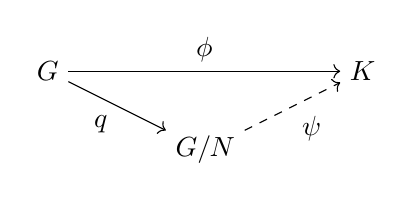
\begin{tikzpicture}
    \node (G) at (0, 1){$G$};
    \node (K) at (4, 1){$K$};
    \node (GN) at (2, 0){$G/N$};
    \draw[->] (G)--(K) node[midway, above]{$\phi$};
    \draw[->] (G)--(GN) node[midway, below left]{$q$};
    \draw[->, dashed] (GN)--(K) node[midway, below right]{$\psi$};
  \end{tikzpicture}
\end{center}

Can we extend this to rings?

Let $\phi \colon R \to S$ be a ring homomorphism and $\ideal$ an ideal of $R$.
Suppose $\ideal \subseteq \ker\phi$.
By the universal property of quotient groups, there is a unique group homomorphism
$\psi \colon R/\ideal \to S$ such that $\phi = \psi \circ q$.

\begin{center}
  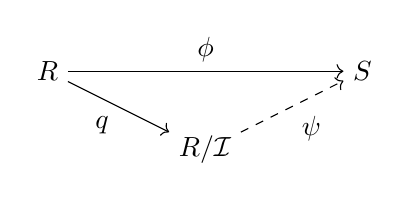
\begin{tikzpicture}
    \node (R) at (0, 1){$R$};
    \node (S) at (4, 1){$S$};
    \node (RI) at (2, 0){$R/\ideal$};
    \draw[->] (R)--(S) node[midway, above]{$\phi$};
    \draw[->] (R)--(RI) node[midway, below left]{$q$};
    \draw[->, dashed] (RI)--(S) node[midway, below right]{$\psi$};
  \end{tikzpicture}
\end{center}

Is $\psi$ a ring homomorphism?

\begin{lem}{}{}
  Let $R, S, T$ be rings.
  Suppose that $\psi_1 \colon R \to T$ is a ring homomorphism and $\psi_2 \colon T \to S$ is a
  group homomorphism, such that $\psi_2 \circ \psi_1$ is a ring homomorphism.
  If $\psi_1$ is surjective, then $\psi_2$ is a ring homomorphism.
\end{lem}

\begin{thmproof}
  Let $\phi = \psi_2 \circ \psi_1$.

  Suppose $x, y \in T$.
  Let $a, b \in R$ such that $\psi_1(a) = x$ and $\psi_1(b) = y$.
  Then $\psi_2(xy) = \psi_2(\psi_1(a)\psi_1(b)) = \psi_2(\psi_1(ab)) = \phi(ab) = \phi(a)\phi(b)
    = \psi_2(\psi_1(a))\psi_2(\psi_1(b)) = \psi_2(x)\psi_2(y)$.

  Also, $\psi_2(1_T) = \psi_2(\psi_1(1_R)) = \phi(1_R) = 1_S$.

  So $\psi_2$ is a ring homomorphism.
\end{thmproof}

As a corollary of the lemma and the universal property of quotient groups:

\begin{thm}{Universal property of quotient rings}{}
  Suppose $\phi \colon R \to S$ is a ring homomorphism and $\ideal$ is an ideal of $R$.
  Let $q \colon R \to R/\ideal$ be the quotient homomorphism.
  Then there is a ring homomorphism $\psi \colon R/\ideal \to S$ such that $\psi \circ q = \phi$ if
  and only if $\ideal \subseteq \ker\phi$.
  Furthermore, if $\psi$ exists then it is unique.
\end{thm}

\begin{thmproof}
  \textbf{Existence:}
  If $\ideal \subseteq \ker\phi$, then $\psi$ exists as a group homomorphism.
  Applying the lemma with $\psi_1 = q$, $\psi_2 = \psi$, and $T = R/\ideal$ shows $\psi$ is a ring
  homomorphism.

  \textbf{Uniqueness:}
  Any ring homomorphism $\psi \colon R/\ideal \to S$ such that $\psi \circ q = \phi$ is equal to the
  unique group homomorphism with this property.

  \textbf{Necessity of $\ideal \in \ker\phi$:}
  If $\psi$ exists, then it is a group homomorphism, so apply the universal property of quotient
  groups.
\end{thmproof}

\pagebreak
\subsection{First isomorphism theorem for rings}

\begin{thm}{First isomorphism theorem for rings}{}
  If $\phi \colon R \to S$ is a ring homomorphism, then there is a ring isomorphism
  $\psi \colon R/\ker\phi \to \Im\phi$ such that $\phi = \psi \circ q$, where
  $q \colon R \to R/\ker\phi$ is the quotient homomorphism.
\end{thm}

\begin{thmproof}
  By the universal property, we have a ring homomorphism $\psi \colon R/\ker\phi \to \Im\phi$ such
  that $\psi \circ q = \phi$.
  From the first isomorphism theorem for groups, there is a group isomorphism
  $\psi' \colon R/\ker\phi \to \Im\phi$ such that $\psi' \circ q = \phi$.
  $\psi$ is also a group homomorphism.
  By the universal property of quotient groups, $\psi = \psi'$, so $\psi$ is bijective.

  (Or, apply the lemma to $\psi'$.)
\end{thmproof}

The first isomorphism theorem is very useful for finding quotient rings.

\begin{prop}{}{}
  Let $R$ be a commutative ring and let $c \in R$.
  Then $R[x]/(x - c)R[x] \cong R$.
\end{prop}

\begin{thmproof}
  $(x - c)R[x] = \ker\ev_c$, where $\ev_c \colon R[x] \to R$ is the evaluation map.
  If $r \in R$, then $\ev_c(r) = r$, so $\Im\ev_c = R$.
  By the first isomorphism theorem, $R[x]/(x - c)R[x] \cong R$.
\end{thmproof}

\begin{ex}
  Let $\ideal = (y - x^2)\Z[x, y] = \{(y - x^2)p(x, y) : p(x, y) \in \Z[x, y]\}$.

  To see that $\ideal$ is an ideal, note that $\ideal = \ker\ev_{x^2}$, where
  $\ev_{x^2} \colon \Z[x, y] = \Z[x][y] \to \Z[x]$ is evaluation at $x^2$.
  (From the recursive definition and our previous investigation.)

  By the proposition, $\Z[x, y]/\ideal \cong \Z[x]$.
\end{ex}

%%%%% Lec 20
\section{Ideals generated by a subset}

\subsection{Ideal generated by a subset}

\begin{prop}{}{}
  Let $\mathcal{F}$ be a family of ideals in a ring $R$.
  Then \[ \bigcap_{\ideal \in \mathcal{F}} \ideal \] is an ideal of $R$.
\end{prop}

\begin{thmproof}
  Homework.
\end{thmproof}

\begin{defn}{ideal generated by a subset}{}
  Let $X \subseteq R$.
  The \hldef{ideal generated by $X$} is
  \[ (X) := \bigcap_{\ideal \in \mathcal{F}} \ideal, \]
  where $\mathcal{F}$ is the set of ideals of $R$ containing $X$.
\end{defn}

Key properties:
\begin{itemize}
  \item By proposition, $(X)$ is an ideal.
  \item By definition, if $\ideal$ is an ideal containing $X$, then
    $X \subseteq (X) \subseteq \ideal$.
    Say that $(X)$ is the smallest ideal containing $X$.
  \item Example: $(0) = (\varnothing) = \{0\}$.
\end{itemize}

Notation:
\begin{itemize}
  \item Sometimes use $\ang{X}$ instead of $(X)$.
  \item If $X = \{f_1, f_2, \ldots\}$, can replace $(X) = (\{f_1, f_2, \ldots\})$ by
    $(f_1, f_2, \ldots)$.
    Example: $(0)$ instead of $(\{0\})$.
\end{itemize}

\begin{prop}{}{}
  If $R$ is a ring and $X \subseteq R$, then
  \[
    (X) = \left\{ \sum_{i = 1}^k s_i x_i t_i : k \geq 0, \ s_i, t_i \in R, \ x_i \in X
      \text{ for } 1 \leq i \leq k \right\}.
  \]
\end{prop}

\begin{cor}{}{}
  If $R$ is a commutative ring and $X \subseteq R$, then
  \[
    (X) = \left\{ \sum_{i = 1}^k r_i x_i : k \geq 0, \ r_i \in R, \ x_i \in X
      \text{ for } 1 \leq i \leq k \right\}.
  \]
\end{cor}

\begin{thmproof}
  $s_i x_i t_i = (s_i t_i) x_i$, so set $r_i = s_i t_i$.
\end{thmproof}

\begin{thmproof}[Proof of proposition.]
  Let $\ideal$ be the set in question.

  First, show $\ideal$ is an ideal.
  Taking $k = 0$, we get $0_R \in \ideal$.
  Suppose $r \in R$ and $x, y \in \ideal$.
  Let $x = \sum_{i = 1}^k s_i x_i t_i$ and $y = \sum_{i = 1}^\ell s_i' y_i t_i'$ for
  $s_i, t_i, s_i', t_i' \in R$ and $x_i, y_i \in X$.
  Then $rx + y = \sum_{i = 1}^k (rs_i) x_i t_i + \sum_{i = 1}^\ell s_i' y_i t_i' \in \ideal$ and
  similarly $xr + y \in \ideal$, so $\ideal$ is an ideal.

  Next, show $(X) \subseteq \ideal$.
  Taking $k = 1$ and $s_1 = t_1 = 1$, we get $X \subseteq \ideal$ so $(X) \subseteq \ideal$.

  Finally, show $\ideal \subseteq (X)$.
  Suppose $k \geq 0$, $s_i, t_i \in R$, and $x_i \in X$ for $1 \leq i \leq k$.
  Since $X \subseteq (X)$, $x_i \in (X)$ means $s_i x_i t_i \in (X)$ for all $1 \leq i \leq k$.
  So $\sum_{i = 1}^k s_i x_i t_i \in (X)$.
  Hence $\ideal \subseteq (X)$.
\end{thmproof}

\pagebreak
\subsection{The sum of ideals}

\begin{defn}{ideal sum}{}
  If $\mathcal{I}, \mathcal{J} \subseteq R$ are ideals, then
  $\mathcal{I} + \mathcal{J} := \{x + y : x \in \mathcal{I}, \ y \in \mathcal{J}\}$.
\end{defn}

\begin{cor}{}{}
  $(\mathcal{I} \cup \mathcal{J}) = \mathcal{I} + \mathcal{J}$ is the smallest ideal containing
  both $\mathcal{I}$ and $\mathcal{J}$.
\end{cor}

\begin{thmproof}
  By proposition, clearly $\mathcal{I} + \mathcal{J} \subseteq (\mathcal{I} \cup \mathcal{J})$.

  For the reverse inclusion, suppose $s_i, t_i \in R$ and $x_i \in \mathcal{I} \cup \mathcal{J}$
  for $1 \leq i \leq k$.
  Let $S = \{1 \leq i \leq k : x_i \in \mathcal{I}\}$, so if $i \in S$, then
  $s_i x_i t_i \in \mathcal{I}$.
  So $\sum_{i \in S} s_i x_i t_i \in \mathcal{I}$, and similarly
  $\sum_{i \not\in S} s_i x_i t_i \in \mathcal{J}$.
  We conclude that $\sum_{i = 1}^k s_i x_i t_i = \sum_{i \in S} s_i x_i t_i +
    \sum_{i \not\in S} s_i x_i t_i \in \mathcal{I} + \mathcal{J}$.
\end{thmproof}

\pagebreak
\subsection{Lattice of ideals}

Ideals of $R$ are ordered by set inclusion $\subseteq$.
The set of ideals of $R$ with order $\subseteq$ is called the \hldef{lattice of ideals} of $R$.

\begin{center}
  \begin{forest}
    [$R$, calign=child, calign child=2
      [$\phantom{\cdots}$, name=2]
      [$\cdots$
        [$(0)$, name=0]
      ]
      [$\phantom{\cdots}$, name=3]
    ]
    \draw (2)--(0);
    \draw (3)--(0);
  \end{forest}
\end{center}

The subgroup below $\ideal_1$ and $\ideal_2$ in the lattice is $\ideal_1 \cap \ideal_2$
(maximal subgroup contained in both).

The subgroup above $\ideal_1$ and $\ideal_2$ is $\ideal_1 + \ideal_2$ (minimal subgroup containing
both).

\pagebreak
\subsection{Quotients by a subset}

We get a new way of constructing rings: take $R/(X)$ for any subset $X$.
We know $R/(X)$ is a unital ring, but when is it non-zero?

From group theory, we know that $R/\ideal$ is zero if and only if $\ideal = R$.
We proved that $\ideal = R$ if and only if $1 \in \ideal$.

\begin{cor}{}{}
  Let $R$ be a ring and $X \subseteq R$.
  Then $R/(X) = \{0\}$ if and only if there are $s_i, t_i \in R$ and $x_i \in X$ for
  $1 \leq i \leq k$ such that
  \[ \sum_{i = 1}^k s_i x_i t_i = 1. \]
\end{cor}

If $R$ is commutative, we can instead just show $\sum_{i = 1}^k r_i x_i = 1$ for $r_i \in R$ and
$x_i \in X$.

\pagebreak
\subsection{Ideals generated by a finite subset}

We often take ideals $(x_1, \ldots, x_n)$ generated by finite sets $\{x_1, \ldots, x_n\}$.

\begin{cor}{}{}
  If $R$ is a commutative ring and $X \subseteq R$, then
  \[
    (X) = \left\{
      \sum_{i = 1}^k r_i x_i : k \geq 0, \ r_i \in R, \ x_i \in X \text{ for } 1 \leq i \leq k
    \right\}.
  \]
\end{cor}

\begin{cor}{}{}
  If $R$ is a commutative ring and $X = \{x_1, \ldots, x_n\} \subseteq R$, then
  \[ (X) = \left\{ \sum_{i = 1}^n r_i x_i : r_i \in R, \ 1 \leq i \leq n \right\}. \]
\end{cor}

\begin{thmproof}
  $\text{RHS} \subseteq (X)$ is clear.
  For the other inclusion, note that $rx_i + r'x_i = (r + r')x_i$, so we can collect like terms;
  if $x_i$ is unneeded, then set $r_i = 0$.
\end{thmproof}

\pagebreak
\subsection{Principal ideals}

\begin{defn}{principal ideal}{}
  An ideal generated by a single element is called a \hldef{principal ideal}.
\end{defn}

If $R$ is a commutative ring, then $(x) = \{rx : r \in R\}$, so a principal ideal $(x)$ is often
denoted by $xR$ or $Rx$.

\begin{ex}
  Let $R = \Z$ and $m \in \Z$.
  Then $(m) = m\Z$ is a principal ideal.

  All subgroups of $\Z$ are of the form $m\Z$ for some $m \in \Z$, so all subgroups of $\Z$ are
  principal ideals.
  In particular, all ideals of $\Z$ are principal ideals.
\end{ex}

\begin{ex}
  If $R$ is commutative and $p(x) \in R[x]$, then $(p) = pR[x]$ is an ideal.
\end{ex}

\pagebreak
\subsection{Principal ideals in non-commutative rings}

If $R$ is non-commutative, then $(x)$ is not necessarily equal to $\{rx : r \in R\}$ since
$xr \in (x)$ for $r \in R$.
But is $(x) = \{sxr : s, r \in R\}$?
In general, no.

\begin{ex}
  Let $E_{11} = \begin{pmatrix} 1 & 0 \\ 0 & 0 \end{pmatrix} \in M_2\R$.

  We know $AE_{11}B$ has rank $\leq 1$ for every $A, B \in M_2\R$, hence
  $\{AE_{11}B : A, B \in M_2\R\} \subsetneq M_2\R$.

  Let $X = \begin{pmatrix} 0 & 1 \\ 1 & 0 \end{pmatrix}$.
  Then $XE_{11}X = \begin{pmatrix} 0 & 0 \\ 0 & 1 \end{pmatrix}$.

  So $E_{11} + XE_{11}X = I \in (E_{11})$, and we conclude that $(E_{11}) = M_2\R$.
\end{ex}

\pagebreak
\subsection{More examples in polynomial rings}

Principal ideals:
\begin{itemize}
  \item
  We've already mentioned the principal ideals $(x - c)\Z[x]$ for $c \in \Z$.
  For example, $x\Z[x]$ is the ideal of polynomials with no constant term.
  \item
  Another good example is $m\Z[x]$ for $m \in \Z$.
  This is
  $m\Z[x] = \{\sum_{i = 0}^n a_i x^i : n \geq 0, \ a_i \in m\Z \text{ for } 0 \leq i \leq n\}$.
  \item
  The previous example doesn't work in $\Q[x]$, though, since $2\Q[x] = \Q[x]$
  ($2 \cdot \frac{1}{2} = 1$).
  Also, $\Z[x]$ is not an ideal in $\Q[x]$ (in general, subrings are very different from ideals).
\end{itemize}

What about non-principal ideals?

In $\Z[x, y]$, $(x, y) = \{p(x, y)x + q(x, y)y : p, q \in \Z[x, y]\}$.
So $(x, y)$ contains $x, y, xy, x^2, y^2$, etc.
Note $p, q$ aren't unique: $xy = 0 + x \cdot y = y \cdot x + 0$.
To see that $(x, y)$ is a proper ideal of $\Z[x, y]$, observe that
\[ (x, y) = \left\{
  \sum_{i, j = 0}^n a_{ij} x^i y^j : n \geq 0, a_{ij} \in \Z \text{ for } 0 \leq i, j \leq n,
    \ a_{00} = 0
\right\}. \]

\begin{exer}{}{}
  Suppose there are polynomials $f, p, q \in \Z[x, y]$ such that $p \cdot f = x$ and
  $q \cdot f = y$.
  Show $f \in \{\pm 1\}$.
\end{exer}

Consequence: the only principal ideal containing $(x, y)$ is $\Z[x, y]$.
In particular, $(x, y)$ is not principal.

All ideals of $\Z$ are principal, whereas $\Z[x, y]$ has non-principal ideals.

What about $\Z[x]$?
Consider the ideal
\begin{align*}
  (2, x) &= \{2p(x) + xq(x) : p, q \in \Z[x]\} \\
  &= \left\{ \sum_{i = 0}^n a_i x^i : n \geq 0, \ a_i \in \Z \text{ for } 0 \leq i \leq n,
    \ a_0 \in 2\Z \right\}.
\end{align*}
Can this ideal be principal?

\begin{exer}{}{}
  Show that if $p, f \in \Z[x]$ such that $p(x)f(x) = 2$, then $f \in \{\pm 1, \pm 2\}$.

  Show that $x \not\in \pm 2\Z[x]$.
\end{exer}

Conclusion: the only principal ideal containing $(2, x)$ is $\Z[x]$.

%%%%% Lec 21
\section{Correspondence, second and third isomorphism theorems}

\subsection{Connecting ideals and homomorphisms (correspondence theorem)}

\begin{prop}{}{}
  Let $\phi \colon R \to S$ be a ring homomorphism.
  \begin{enumerate}
    \item If $\ideal$ is an ideal of $S$, then $\phi^{-1}(\ideal)$ is an ideal of $R$.
    \item If $\ideal$ is an ideal of $R$ and $\phi$ is surjective, then $\phi(\ideal)$ is an ideal
      of $S$.
  \end{enumerate}
\end{prop}

\begin{thmproof}
  Homework.
  (Also provide counterexample for (2) when $\phi$ is not surjective.)
\end{thmproof}

Recall from group theory:

\begin{thm}{Correspondence theorem for groups}{}
  Let $\phi \colon G \to H$ be a surjective homomorphism.
  Then there is a bijection
  \begin{center}
    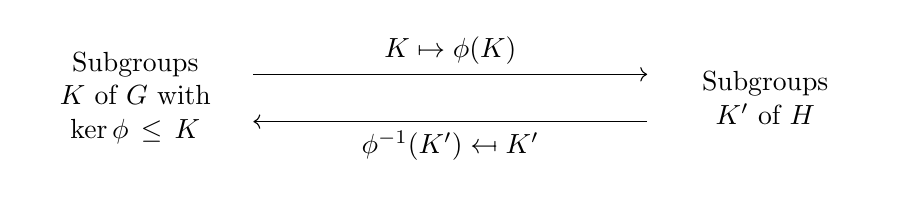
\begin{tikzpicture}
      \node[align=center, text width=2.5cm] at (0, 0){Subgroups $K$ of $G$ with $\ker\phi \leq K$};
      \node[align=center, text width=2.5cm] at (8, 0){Subgroups $K'$ of $H$};
      \draw[->] (1.5, 0.3)--(6.5, 0.3) node[midway, above]{$K \mapsto \phi(K)$};
      \draw[->] (6.5, -0.3)--(1.5, -0.3) node[midway, below]{$\phi^{-1}(K') \mapsfrom K'$};
    \end{tikzpicture}
  \end{center}
  Furthermore, if $\ker\phi \leq K, K_1, K_2 \leq G$ then
  \begin{enumerate}
    \item $K_1 \leq K_2 \iff \phi(K_1) \leq \phi(K_2)$,
    \item $\phi(K_1 \cap K_2) = \phi(K_1) \cap \phi(K_2)$, and
    \item $K$ is normal $\iff$ $\phi(K)$ is normal.
  \end{enumerate}
\end{thm}

We can get a version for rings immediately.

\begin{thm}{Correspondence theorem for rings}{}
  Let $\phi \colon R \to S$ be a surjective ring homomorphism.
  Then there is a bijection
  \begin{center}
    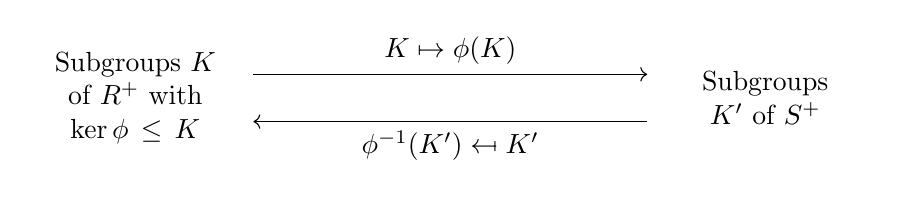
\begin{tikzpicture}
      \node[align=center, text width=2.5cm]
        at (0, 0){Subgroups $K$ of $R^+$ with $\ker\phi \leq K$};
      \node[align=center, text width=2.5cm] at (8, 0){Subgroups $K'$ of $S^+$};
      \draw[->] (1.5, 0.3)--(6.5, 0.3) node[midway, above]{$K \mapsto \phi(K)$};
      \draw[->] (6.5, -0.3)--(1.5, -0.3) node[midway, below]{$\phi^{-1}(K') \mapsfrom K'$};
    \end{tikzpicture}
  \end{center}
  Furthermore, if $\ker\phi \leq K, K_1, K_2 \leq R^+$, then $K$ is an ideal if and only if
  $\phi(K)$ is an ideal.
\end{thm}

\begin{thmproof}
  Apply proposition and use the fact that $K = \phi^{-1}(\phi(K))$.
\end{thmproof}

In the special case of $q \colon R \to R/\ideal$, if $\ideal \subseteq \mathcal{K} \leq R^+$, then
$\mathcal{K}$ is an ideal of $R$ if and only if $\mathcal{K}/\ideal$ is an ideal of $R/\ideal$.

\begin{ex}
  Let $R$ be a commutative ring.
  What are the ideals of $R[x]$ containing $(x)$?

  $(x)$ is the kernel of the surjective homomorphism $\ev_{x = 0} \colon R[x] \to R$.
  So ideals of $R[x]$ containing $(x)$ correspond to ideals $\ideal$ of $R$.

  If $\ideal$ is an ideal of $R$, what is the corresponding ideal in $R[x]$?

  Answer:
  \begin{align*}
    \ev_{x = 0}^{-1}(\ideal) &= \{f \in R[x] : f(0) \in \ideal\} \\
    &= \left\{ \sum_{i = 0}^n a_i x^i : n \geq 0, \ a_i \in R \text{ for } 0 \leq i \leq n,
      \ a_0 \in \ideal \right\}.
  \end{align*}
\end{ex}

\pagebreak
\subsection{Second isomorphism theorem}

Recall from group theory:

\begin{thm}{Second isomorphism theorem for groups}{}
  Suppose $H \subseteq N_G(K)$.
  Then $HK \leq G$, $K \trianglelefteq HK$, and $H \cap K \trianglelefteq H$.
  Furthermore, if $i_H \colon H \to HK$ is the inclusion and $q_1 \colon H \to H/(H \cap K)$ and
  $q_2 \colon HK \to HK/K$ are the quotient maps, then there is an isomorphism
  $\psi \colon H/(H \cap K) \to HK/K$ such that $\psi \circ q_1 = q_2 \circ i_H$.
\end{thm}

\begin{center}
  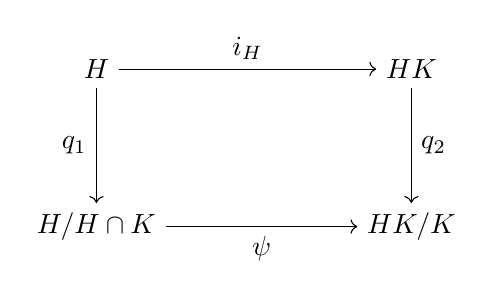
\begin{tikzpicture}
    \node (H) at (0, 2){$H$};
    \node (HK) at (4, 2){$HK$};
    \node (HHK) at (0, 0){$H/H \cap K$};
    \node (HKK) at (4, 0){$HK/K$};
    \draw[->] (H)--(HHK) node[midway, left]{$q_1$};
    \draw[->] (H)--(HK) node[midway, above]{$i_H$};
    \draw[->] (HK)--(HKK) node[midway, right]{$q_2$};
    \draw[->] (HHK)--(HKK) node[midway, below]{$\psi$};
  \end{tikzpicture}
\end{center}

Let's restate this for abelian groups with additive notation.

\begin{thm}{Second isomorphism theorem for abelian groups}{}
  Suppose $H, K \leq G$.
  Then $H + K \leq G$, and furthermore, if $i_H \colon H \to H + K$ is the inclusion,
  $q_1 \colon H \to H/H \cap K$ and $q_2 \colon H + K \to H + K/K$ are the quotient maps, then
  there is an isomorphism $\psi \colon H/H \cap K \to H + K/K$ such that
  $\psi \circ q_1 = q_2 \circ i_H$.
\end{thm}

\begin{center}
  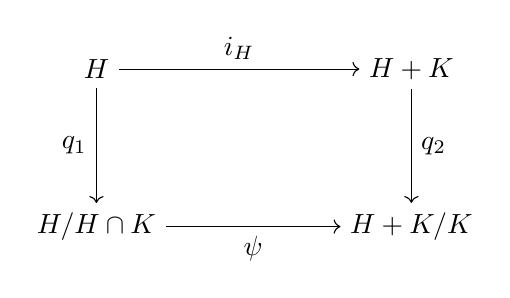
\begin{tikzpicture}
    \node (H) at (0, 2){$H$};
    \node (HK) at (4, 2){$H + K$};
    \node (HHK) at (0, 0){$H/H \cap K$};
    \node (HKK) at (4, 0){$H + K/K$};
    \draw[->] (H)--(HHK) node[midway, left]{$q_1$};
    \draw[->] (H)--(HK) node[midway, above]{$i_H$};
    \draw[->] (HK)--(HKK) node[midway, right]{$q_2$};
    \draw[->] (HHK)--(HKK) node[midway, below]{$\psi$};
  \end{tikzpicture}
\end{center}

Now we can extend this to rings.

\begin{thm}{Second isomorphism theorem for rings}{}
  Let $S$ be a subring of $R$ and let $\ideal$ be an ideal of $R$.
  Then $S + \ideal$ is a subring of $R$ and $S \cap \ideal$ is an ideal of $S$.
  Furthermore, if $i_S \colon S \to S + \ideal$ is the inclusion and
  $q_1 \colon S \to S/S \cap \ideal$ and $q_2 \colon S + \ideal \to S + \ideal/\ideal$ are the
  quotient maps, then there is a (ring) isomorphism
  $\psi \colon S/S \cap \ideal \to S + \ideal/\ideal$ such that $\psi \circ q_1 = q_2 \circ i_S$.
\end{thm}

\begin{center}
  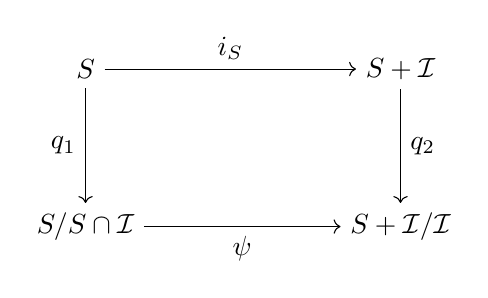
\begin{tikzpicture}
    \node (S) at (0, 2){$S$};
    \node (SI) at (4, 2){$S + \ideal$};
    \node (SSI) at (0, 0){$S/S \cap \ideal$};
    \node (SII) at (4, 0){$S + \ideal/\ideal$};
    \draw[->] (S)--(SSI) node[midway, left]{$q_1$};
    \draw[->] (S)--(SI) node[midway, above]{$i_S$};
    \draw[->] (SI)--(SII) node[midway, right]{$q_2$};
    \draw[->] (SSI)--(SII) node[midway, below]{$\psi$};
  \end{tikzpicture}
\end{center}

Here $S + \ideal = \{s + x : s \in S, \ x \in \ideal\}$ (same definition as for ideals).

\begin{thmproof}
  $S, \ideal$ are subgroups of $R^+$ and $S + \ideal$ is a subgroup of $R^+$.

  To show that $S + \ideal$, note that $1 \in S + \ideal$.
  If $x, y \in S + \ideal$, then $x = s + a$ and $y = t + b$ for some $s, t \in S$ and
  $a, b \in \ideal$.
  So $xy = st + (st + at + ab) \in S + \ideal$ and hence $S + \ideal$ is a subring.

  Exercise: show $S \cap \ideal$ is an ideal of $S$.

  By second isomorphism theorem for groups, there is an isomorphism
  $\psi \colon S/S \cap \ideal \to S + \ideal/\ideal$ such that $\psi \circ q_1 = q_2 \circ i_S$.

  By applying the lemma below, we see $\psi$ is a ring isomorphism.
\end{thmproof}

\begin{lem}{From universal property of quotient rings}{}
  Let $R, S, T$ be rings.
  Suppose that $\psi_1 \colon R \to T$ is a ring homomorphism and $\psi_2 \colon T \to S$ is a
  group homomorphism such that $\psi_2 \circ \psi_1$ is a ring homomorphism.
  If $\psi_1$ is surjective, then $\psi_2$ is a ring homomorphism.
\end{lem}

\begin{ex}
  Let $\mathcal{J}$ be an ideal of a commutative ring $R$.

  Let $\ideal = \{f \in R[x] : f(0) \in \mathcal{J}\} = \ev_0^{-1}(\mathcal{J})$.

  Then
  \begin{itemize}
    \item $R$ is a subring of $R[x]$,
    \item $R + \ideal = R[x]$, and
    \item $R \cap \ideal = \mathcal{J}$.
  \end{itemize}
  So $R/\mathcal{J} \cong R[x]/\ideal$ by the second isomorphism theorem.
\end{ex}

\pagebreak
\subsection{Third isomorphism theorem}

From group theory:

\begin{thm}{Third isomorphism theorem for groups}{}
  Let $N \trianglelefteq G$ and $N \leq K \trianglelefteq G$.
  Let
  \begin{itemize}
    \item $q_1$ be the quotient map $G \to G/N$,
    \item $q_2$ be the quotient map $G/N \to (G/N)/(K/N)$, and
    \item $q_3$ be the quotient map $G \to G/K$.
  \end{itemize}
  Then there is an isomorphism $\psi \colon G/K \to (G/N)/(K/N)$ such that
  $\psi \circ q_3 = q_2 \circ q_1$.
\end{thm}

\begin{center}
  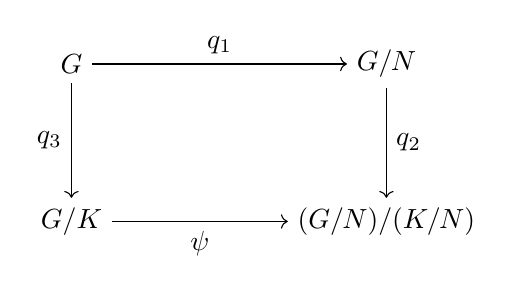
\begin{tikzpicture}
    \node (G) at (0, 2){$G$};
    \node (GN) at (4, 2){$G/N$};
    \node (GK) at (0, 0){$G/K$};
    \node (GNKN) at (4, 0){$(G/N)/(K/N)$};
    \draw[->] (G)--(GK) node[midway, left]{$q_3$};
    \draw[->] (G)--(GN) node[midway, above]{$q_1$};
    \draw[->] (GN)--(GNKN) node[midway, right]{$q_2$};
    \draw[->] (GK)--(GNKN) node[midway, below]{$\psi$};
  \end{tikzpicture}
\end{center}

Now for rings:


\begin{thm}{Third isomorphism theorem for groups}{}
  Suppose $\ideal \subseteq \mathcal{K}$ are ideals of a ring $R$, and let
  \begin{itemize}
    \item $q_1$ be the quotient map $R \to R/\ideal$,
    \item $q_2$ be the quotient map $R/\ideal \to (R/\ideal)/(\mathcal{K}/\ideal)$, and
    \item $q_3$ be the quotient map $R \to R/\mathcal{K}$.
  \end{itemize}
  Then there is a (ring) isomorphism $\psi \colon R/\mathcal{K} \to (R/\ideal)/(\mathcal{K}/\ideal)$
  such that $\psi \circ q_3 = q_2 \circ q_1$.
\end{thm}

\begin{center}
  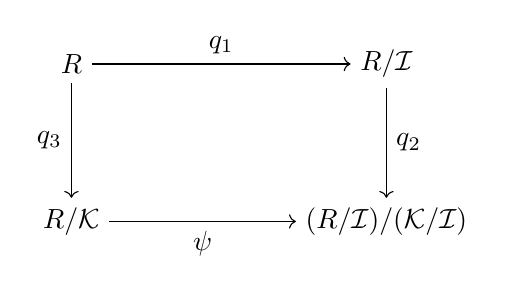
\begin{tikzpicture}
    \node (R) at (0, 2){$R$};
    \node (RI) at (4, 2){$R/\ideal$};
    \node (RK) at (0, 0){$R/\mathcal{K}$};
    \node (RIKI) at (4, 0){$(R/\ideal)/(\mathcal{K}/\ideal)$};
    \draw[->] (R)--(RK) node[midway, left]{$q_3$};
    \draw[->] (R)--(RI) node[midway, above]{$q_1$};
    \draw[->] (RI)--(RIKI) node[midway, right]{$q_2$};
    \draw[->] (RK)--(RIKI) node[midway, below]{$\psi$};
  \end{tikzpicture}
\end{center}

\begin{thmproof}
  Apply the lemma from the universal property of quotient rings again.
\end{thmproof}

\begin{ex}
  $(\Z/mn\Z)/(m\Z/mn\Z) \cong \Zmod{m}$ as groups, and also as rings.
\end{ex}

\begin{ex}
  As in the previous example, let $\mathcal{J}$ be an ideal of $R$ and
  $\ideal = \ev_0^{-1}(\mathcal{J}) \subseteq R[x]$.

  Now $\ideal$ contains $(x)$, so by the third isomorphism,
  $R[x]/\ideal \cong (R[x]/(x))/(\ideal/(x))$.

  By first isomorphism theorem, $R[x]/(x) \cong R$ since $(x) = \ker\ev_0$.
  This isomorphism sends $f(x) + (x) \in R[x]/(x)$ to $\ev_0(f) = f(0)$, and hence identifies
  $\ideal/(x)$ with $\mathcal{J}$.

  Conclusion: $R[x]/\ideal \cong (R/(x))/(\ideal/(x)) \cong R/\mathcal{J}$.

  Exercise: show that this isomorphism is the same as the isomorphism
  $R/\mathcal{J} \cong R[x]/\ideal$ from the second isomorphism theorem.
\end{ex}

\week{Maximal and Prime Ideals}

%%%%% Lec 22
\section{Maximal ideals and fields}

\subsection{Constructing complex numbers from real numbers}

From last week: we can construct new rings $R/(X)$ by taking $X \subseteq R$.
What sets $X$ might we like to look at?

Suppose we didn't know about $\C$, and we want a square root of $-1$.
We want to take $\R$ and add an element $x$ such that $x^2 = -1$.

So let's look at $\R[x]/(x^2 + 1)$ (note $x^2 + 1 = 0 \iff x^2 = -1$).
If we look at $\overline{x} = [x]$ in $\R[x]/(x^2 + 1)$, then
\[
  \overline{x}^2 + 1 = [x]^2 + [1] = [x^2 + 1] = x^2 + 1 + (x^2 + 1) = (x^2 + 1) = 0.
\]
What ring is $\R[x]/(x^2 + 1)$?

\begin{thm}{}{}
  $\R[x]/(x^2 + 1) \cong \C$.
\end{thm}

If we didn't know about $\C$, we could use $\R[x]/(x^2 + 1)$ as the definition.

\pagebreak
\subsection{The complex numbers}

Let's clarify what $\C$ is:
\begin{itemize}
  \item $\C = \{a + bi : a, b \in \R\}$
  \item $(a + bi) + (c + di) = (a + c) + (b + d)i$
  \item $(a + bi)(c + di) = (ac - bd) + (ad + bc)i$
\end{itemize}

How does $\R[x]/(x^2 + 1)$ correspond to $\C$?
We know that $\overline{x}$ acts like $i$.

\begin{lem}{}{}
  Every element of $\R[x]/(x^2 + 1)$ can be written uniquely in the form $a + b\overline{x}$ for
  some $a, b \in \R$.
\end{lem}

\begin{thmproof}
  \textbf{Existence:}
  Since the quotient map $\R[x] \to \R[x]/(x^2 + 1)$ is surjective, every element of
  $\R[x]/(x^2 + 1)$ can be written as $\sum_{i = 0}^n a_i \overline{x}^i$.
  (Note the bar on $a_i$ is dropped for brevity.)

  If $n \geq 2$, then $a_n x^{n - 2}(x^2 + 1) \in (x^2 + 1)$, so
  $a_n \overline{x}^n + a_n \overline{x}^{n - 2} = 0$.
  Thus
  \begin{align*}
    \sum_{i = 0}^n a_i \overline{x}^i
    &= \sum_{i = 0}^{n} a_i \overline{x}^i - (a_n \overline{x}^n + a_n \overline{x}^{n - 2}) \\
    &= 0 \cdot \overline{x}^n + a_{n - 1} \overline{x}^{n - 1}
      + (a_{n - 2} - a_n) \overline{x}^{n - 2} + \cdots.
  \end{align*}
  We can lower $n$ until we get $\sum_{i = 0}^n a_i \overline{x}^i = a + b\overline{x}$ for some
  $a, b$.

  \textbf{Uniqueness:}
  Suppose $a + b\overline{x} = c + d\overline{x}$.
  Then $(a - c) + (b - d)\overline{x} = 0$, so $(a - c) + (b - d)x \in (x^2 + 1)$.

  If $f \in (x^2 + 1)$ and $f \neq 0$, then $f = g(x^2 + 1)$ for $g \in \R[x]$ with $g \neq 0$.
  So $\deg(f) = \deg(g) + \deg(x^2 + 1) \geq 2$.

  Hence every non-zero element of $(x^2 + 1)$ has degree $\geq 2$.
  Then the only way $(a - c) + (b + d)x$ can be in $(x^2 + 1)$ is if it is zero, so
  $a = c$ and $b = d$.
\end{thmproof}

Now for the theorem:

\begin{thm}{}{}
  $\R[x]/(x^2 + 1) \cong \C$.
\end{thm}

\begin{thmproof}
  Since $\R$ is a subring of $\C$, we can consider $\R[x]$ as a subring of $\C[x]$.

  Let $j \colon \R[x] \hookrightarrow \C[x]$ be the inclusion.
  Let $\phi = \ev_{x = i} \circ j \colon \R[x] \to \C[x] \to \C$.
  Then $\phi(x) = i$, so $\phi(x^2 + 1) = i^2 + 1 = 0$.
  So $x^2 + 1 \in \ker\phi$, so $(x^2 + 1) \subseteq \ker\phi$.

  By the universal property of quotient rings, there is a homomorphism
  $\psi \colon \R[x]/(x^2 + 1) \to \C$ such that $\psi \circ q = \phi$.
  So $\psi(a + b\overline{x}) = \phi(a + bx) = a + bi$.
  By the lemma, $\psi$ is a bijection.
\end{thmproof}

This is a common line of proof (see Homework \#4 Q9).

\pagebreak
\subsection{Generalizations}

We constructed $\C$ by asking for an element $x$ such that $x^2 + 1 = 0$.

If we start from a field $\mathbb{K}$, can we ask for an element $x$ satisfying any polynomial
equation(s), and then just cosntruct a ring containing $\mathbb{K}$ with such an element?

Yes!
But the ring might be zero if we ask for too much.

\begin{ex}
  \begin{itemize}
    \item $1 \neq 0$ in $\mathbb{K}[x]/(x^2 + 1)$ as we've seen.
    \item If $p$ is a polynomial of degree $n \geq 1$, then $\mathbb{K}[x]/(p)$ is a
      $\mathbb{K}$-vector space of dimension $n$ (exercise similar to lemma).
      So $1 \neq 0$ in $\mathbb{K}[x]/(p)$.
    \item $1 = 0$ in $\mathbb{K}[x]/(x^2 + 1, x^3 + x + 1)$, since
      $x^3 + x + 1 - x(x^2 + 1) = 1 \in (x^2 + 1, x^3 + x + 1)$.
  \end{itemize}
\end{ex}

\pagebreak
\subsection{Maximal ideals}

Let $\ideal$ be an ideal of a commutative ring $R$.
When is $R/\ideal$ a field?

We know that the only ideals in a field $\mathbb{K}$ are $(0)$ and $\mathbb{K}$.
Suppose $\mathbb{K} = R/\ideal$ is a field, and $q \colon R \to \mathbb{K}$ is the quotient map.
By the correspondence theorem, the only ideals of $R$ containing $\ideal$ are
$q^{-1}((0)) = \ker q = \ideal$ and $q^{-1}(\mathbb{K}) = R$.

\begin{defn}{maximal ideal}{}
  An ideal $\ideal$ of a ring $R$ is \hldef{maximal} if the only ideals containing $\ideal$ are
  $\ideal$ are $R$.
\end{defn}

Intuition: a maximal ideal is a maximal proper ideal under $\subseteq$.

\begin{lem}{}{}
  If $R/\ideal$ is a field, then $\ideal$ is maximal.
\end{lem}

\pagebreak
\subsection{Ideals in fields}

\begin{prop}{}{}
  A commutative ring $R$ is a field if and only if $1 \neq 0$, and the only ideals in $R$ are $(0)$
  and $R$.
\end{prop}

Requiring $1 \neq 0$ is the same as requiring $(0) \neq R$.

\begin{thmproof}
  We already saw the forward implication.

  For the reverse, suppose $x \in R$ wher $x \neq 0$.
  Then $(x) = R$.
  Then $1 \in (x) = xR$, so there is $y \in R$ such that $xy = 1$.
  So $x$ is a unit.
  Since all non-zero elements of $R$ are units, $R$ is a field.
\end{thmproof}

\pagebreak
\subsection{Maximal ideals and fields}

\begin{thm}{}{}
  Let $\ideal$ be an ideal in a commutative ring $R$.
  Then $R/\ideal$ is a field if and only if $\ideal$ is maximal.
\end{thm}

\begin{thmproof}
  By correspondence theorem, the only ideals of $R/\ideal$ are $(0)$ and $R/\ideal$ if and only if
  the only ideals of $R$ containing $\ideal$ are $\ideal$ and $R$.
  So by the proposition, $R/\ideal$ is a field if and only if $\ideal$ is maximal.
\end{thmproof}

\begin{ex}
  \begin{itemize}
    \item $\mathbb{K}[x]/(x - c) \cong \mathbb{K}$ for all $c \in \mathbb{K}$, so $(x - c)$ is a
      maximal ideal of $\mathbb{K}[x]$ for any field $\mathbb{K}$.
    \item $\mathbb{R}[x]/(x^2 + 1) \cong \C$, so $(x^2 + 1)$ is a maximal ideal of $\R[x]$.
  \end{itemize}
\end{ex}

\begin{ex}
  $\Z[x]/(x) \cong \Z$ is not a field, so $(x)$ is not a maximal ideal of $\Z[x]$.

  Indeed, we know that $(x) \subsetneq (2, x) \subsetneq \Z[x]$.
  We also know that $(2, x) = \{f \in \Z[x] : f(0) \in (2)\} = \ev_{x = 0}^{-1}((2))$ for ideal
  $(2) \subseteq \Z$.
  By the second isomorphism theorem, $\Z[x]/(2, x) \cong \Zmod{2}$, which is a field.

  Exercise: $\Z[x]/(n, x) \cong \Zmod{n}$ and hence $(n, x)$ is maximal for $n \in \Z$ if and only
  if $n$ is prime.
\end{ex}

\begin{ex}
  If $R$ is commutative ring, we have
  \[
    \ev_{(a, b)} = \ev_{x = a} \circ \ev_{y = b} \colon R[x, y] = R[x][y] \to R[x] \to R.
  \]
  Then $\ker\ev_{(a, b)} = \ev_{(a, b)}^{-1}((0)) = \ev_{y = b}^{-1}((x - a))
    = \{f \in R[x][y] : f(x, b) \in (x - a)R[x]\} = (x - a, y - b)$.
  By the first isomorphism theorem, $R[x, y]/(x - a, y - b) \cong R$.
  So $(x - a, y - b)$ is a maximal ideal of $R[x, y]$ if and only if $R$ is a field.

  For $(y - x^2) \subseteq R[x, y]$, we know $R[x, y]/(y - x^2) \cong R[x]$.
  $R[x]$ is not a field since $x$ is not a unit.
  So $(y - x^2)$ is not maximal.
  (Indeed, $(y - x^2) \subsetneq (x, y)$.)
\end{ex}

\begin{ex}
  Let $c \in \R$.
  In the homework, you'll show
  \[
    \R[x]/(x^2 - c) \cong \begin{cases}
      \C & c < 0 \\
      \R \times \R & c > 0 \\
      \R[x]/(x^2) \quad & c = 0
    \end{cases}.
  \]
  Exercise: $\R \times \R$ and $\R[x]/(x^2)$ are not fields.
  Hence $\R[x]/(x^2 - c)$ is a field if and only if $c < 0$.
  So $(x^2 - c)$ is maximal if and only if $c < 0$.

  Exercise: find proper ideals properly containing $(x^2 - c)$ for $c \geq 0$.
\end{ex}

\pagebreak
\subsection{Partially-ordered sets}

\begin{defn}{partial order}{}
  A \hldef{partial order} on a set $X$ is a relation $\leq$ on $X$ such that for all
  $x, y, z \in X$:
  \begin{enumerate}
    \item $x \leq x$;
    \item if $x \leq y$ and $y \leq x$, then $x = y$; and
    \item if $x \leq y$ and $y \leq z$, then $x \leq z$.
  \end{enumerate}
  We say that $x < y$ if $x \leq y$ and $x \neq y$.

  A \hldef{maximal element of a subset} $S \subseteq X$ is an element $x \in S$ such that if
  $x \leq y$ for $y \in S$, then $x = y$.

  An \hldef{upper bound of a subset} $S \subseteq X$ is an element $x \in X$ such that $y \leq x$
  for all $y \in S$.

  A \hldef{maximum element of a subset} $S \subseteq X$ is an element $x \in S$ which is an upper
  bound for $S$ (unique if it exists).
\end{defn}

A maximum element (if it exists) of a subset $X$ is maximal.
But a subset $S$ can have maximal elements without having a maximum element.

\begin{ex}
  Consider $2^{\{1, 2\}} = \{\varnothing, \{1\}, \{2\}, \{1, 2\}\}$ ordered by $\subseteq$.

  Then $\{1, 2\}$ is a maximum element for $2^{\{1, 2\}}$, but the subset
  $\{\varnothing, \{1\}, \{2\}\}$ has no maximum element.
  Instead it has two maximal elements: $\{1\}$ and $\{2\}$.
\end{ex}

Ideals of a ring $R$ are ordered under $\subseteq$.
$R$ is a maximum element for the whole set.
We are more interested in the set of proper ideals ordered under $\subseteq$.

\pagebreak
\subsection{Proper ideals ordered under inclusion}

Let $R$ be a non-zero ring, so the set of proper ideals is non-empty.
Does the set of proper ideals of $R$ have a maximum element?
Once a set has more than one maximal element, it can't have a maximum.

\begin{ex}
  $\Zmod{n}$ is a field if and only if $n$ is prime.
  So $(n)$ is maximal if and only if $n$ is prime.
  So $(2)$ and $(3)$ are both maximal.
\end{ex}

Does the set of proper ideals always have a maximal element?

\pagebreak
\subsection{Maximal elements for the set of proper ideals?}

Does the set of proper ideals always have a maximal element?
Maybe we can construct one:
\begin{itemize}
  \item Pick a proper ideal $\ideal_0$.
  \item If $\ideal_0$ is not maximal, find a proper ideal $\ideal_1$ with
    $\ideal_0 \subsetneq \ideal_1$.
  \item Continue until we get to a maximal element.
\end{itemize}

Of course, this might not work.
We might be in a poset (partially ordered set) like $(\N, \leq)$, where we have infinitely long
increasing sequences like $1 < 2 < 3 < \cdots$.
In that case, we're only guaranteed to get a sequence
$\ideal_0 \subsetneq \ideal_1 \subsetneq \ideal_2 \subsetneq \cdots$ of proper ideals.

\pagebreak
\subsection{Chains of ideals}

If $x_0 \leq x_1 \leq x_2 \leq \cdots$ in a partially ordered set $X$, then the subset
$S = \{x_0, x_1, x_2, \ldots\}$ is a chain.

\begin{defn}{chain}{}
  If $(X, \leq)$ is a partially ordered set, we say that a subset $S \subseteq X$ is a \hldef{chain}
  if for every $s, t \in S$, either $s \leq t$ or $t \leq s$ (or both).
\end{defn}

Is the set of proper ideals like $\N$, a chain with no upper bound?

\begin{lem}{}{}
  Let $R$ be a commutative ring, and let $\mathcal{F}$ be a chain of ideals.
  Then
  \[ \bigcup_{\ideal \in \mathcal{F}} \ideal \]
  is an ideal of $R$.
\end{lem}

\begin{thmproof}
  Homework.
\end{thmproof}

Note that this doesn't work if $\mathcal{F}$ is not a chain, since the union of ideals is typically
not closed under addition.

\begin{ex}
  $(2) \cup (3) \subseteq \Z$ doesn't contain $5 = 2 + 3$.
\end{ex}

If $\mathcal{F}$ is a chain of proper ideals, then $1 \not\in \ideal$ for all
$\ideal \in \mathcal{F}$.
So $1 \not\in \bigcup_{\ideal \in \mathcal{F}} \ideal$.

\begin{cor}{}{}
  If $\mathcal{F}$ is a chain of proper ideals of $R$, then there is a proper ideal which is an
  upper bound for $\mathcal{F}$.
\end{cor}

Suppose we try to construct a maximal ideal, and end up with a sequence
$\ideal_0 \subsetneq \ideal_1 \subsetneq \ideal_2 \subsetneq \cdots$ of proper ideals.

By the corollary, there is a proper ideal $\mathcal{J}_0$ which is an upper bound for
$\{\ideal_0, \ideal_1, \ldots\}$, that is, $\ideal_k \subseteq \mathcal{J}_0$ for all $k$.

If $\mathcal{J}_0$ is maximal, then we are done.
If not, we can find a proper ideal $\mathcal{J}_1$ with $\mathcal{J}_0 \subsetneq \mathcal{J}_1$,
and our search continues.

Is this going to end?
It looks like we face a never-ending (infinite) succession of choices.
We need some help.

\pagebreak
\subsection{Zorn's lemma}

\begin{axiom}{Axiom of choice}{}
  Let $X \subseteq 2^Y$ for some $Y$, such that if $A \in X$, then $A \neq \varnothing$.
  Then there is a function $f \colon X \to Y$ such that $f(A) \in A$ for all $A \in X$.
\end{axiom}

The function $f$ is called a \hldef{choice function} (it ``chooses'' an element from each set).
We rarely use the axiom of choice in this form.
However, it has a number of useful equivalent formulation:

\begin{axiom}{Equivalent form of the axiom of choice \#1}{}
  A function $f \colon X \to Y$ is surjective if and only if it has a right inverse.
\end{axiom}

(We called this a theorem earlier in the course because the axiom of choice is one of our standard
axioms.)

\begin{axiom}{Equivalent form of the axiom of choice \#2: Zorn's lemma}{}
  Let $(X, \leq)$ be a partially ordered set, such that if $S$ is a chain in $X$, then there is an
  element $x \in X$ which is an upper bound for $S$.
  Then $X$ contains a maximal element.
\end{axiom}

\pagebreak
\subsection{Maximal elements for the set of proper ideals, continued}

\begin{prop}{}{}
  Suppose that $\mathcal{J}$ is a proper ideal in a commutative ring $R$.
  Then there is a maximal ideal $\mathcal{K}$ of $R$ containing $\mathcal{J}$.
\end{prop}

\begin{thmproof}
  Let $\mathcal{P} = \{\ideal \subsetneq R : \ideal \text{ is an ideal and }
    \mathcal{J} \subseteq \ideal\}$, ordered under $\subseteq$.
  Let $\mathcal{F}$ be a chain in $\mathcal{P}$.

  By the lemma, $\ideal' = \bigcup_{\ideal \in \mathcal{F}} \ideal$ is an ideal of $R$.
  Clearly $\mathcal{J} \subseteq \ideal'$, and since $1 \not\in \ideal'$ we have that
  $\ideal' \in \mathcal{P}$.
  So $\ideal'$ is an upper bound for $\mathcal{F}$ in $\mathcal{P}$.)
  By Zorn's lemma, $\mathcal{P}$ has a maximal element.
\end{thmproof}

\begin{ex}
  Take $(0)$ in $\Z$.
  Then $(0)$ is contained in $(p)$ for any prime $p$, all of which are maximal.
  So the ideal $\mathcal{K}$ in the proposition isn't necessarily unique.
\end{ex}

In particular, every non-zero commutative ring has a maximal ideal.
Or equivalently:

\begin{cor}{}{}
  For every non-zero commutative ring $R$, there is a field $\mathbb{K}$ such that there is a
  homomomorphism $\phi \colon R \to \mathbb{K}$.
\end{cor}

\begin{thmproof}
  Take $\ideal$ to be a maximal ideal of $R$, and let $\phi \colon R \to R/\ideal$ be the quotient
  map.
\end{thmproof}

%%%%% Lec 23
\section{Prime ideals and integral domains}

\subsection{Zero divisors}

If $\mathbb{K}$ is a field and $f, g \in \mathbb{K}[x]$, then $\deg(fg) = \deg(f) + \deg(g)$.

In contrast, in an arbitrary ring like $R = \Zmod{6}$, we can have things like
$(1 + 2x)(1 + 3x) = 1 + 5x + 6x^2 = 1 - x$.
This happens when there are elements $x, y \in R \setminus \{0\}$ with $xy = 0$.

\begin{defn}{zero divisor}{}
  Let $R$ be a ring.
  A non-zero element $x \in R$ is a \hldef{zero divisor} if there is a non-zero element $y \in R$
  such that $xy = 0$ or $yx = 0$.
\end{defn}

That is, $x$ (and $y$) divide 0.

\begin{ex}
  If $n$ is not prime, then $n = ab$ for $2 \leq a, b < n$.
  So $[a], [b] \neq 0$ in $\Zmod{n}$, but $[a] \cdot [b] = [ab] = 0$, so $[a], [b]$ are zero
  divisors.
\end{ex}

\begin{ex}
  If $R$ and $S$ are non-zero rings and $a \neq 0$ in $R$ and $b \neq 0$ in $S$, then
  $(a, 0)$ and $(0, b)$ are non-zero in the product ring $R \times S$.

  But $(a, 0) \cdot (0, b) = (0, 0) = 0$ in $R \times S$, so $(a, 0)$ and $(0, b)$ are zero
  divisors.
\end{ex}

\begin{ex}
  For any ring $R$, $\overline{x}$ is a zero divisor in $R[x]/(x^2)$ since $\overline{x}^2 = 0$.
\end{ex}

\begin{ex}
  For any ring $R$, $\overline{x}$ and $\overline{y}$ are zero divisors in $R[x]/(xy)$.
\end{ex}

For these examples, we still need to show $\overline{x}$ or $\overline{y}$ are non-zero; there are
techniques for this later and on the homework.

\begin{ex}
  Suppose $\mathbb{K}$ is a field.
  Let $E_{ij} \in M_n\mathbb{K}$ be the matrix with a 1 in position $ij$ and 0's elsewhere.

  Then $E_{ij}E_{k\ell} = \delta_{jk}E_{i\ell}$, so $E_{ij}$ is a zero divisor for all $i, j$
  as long as $n \geq 2$.

  Exercise: show that $A \in M_n\mathbb{K}$ is a zero divisor if and only if the rank of $A$ is
  less than $n$ (i.e., $A$ is not invertible).
\end{ex}

\begin{ex}
  Let $G$ be a group, and let $g \in G \setminus \{e\}$ with $\abs{g} = 2$.

  Then $(e + g)(e - g) = e - g^2 = e - e = 0$ in $\Z G$.

  \textbf{Kaplansky zero divisor conjecture}: if every element of $G \setminus \{e\}$ has infinite
  order, and $\mathbb{K}$ is a field, then $\mathbb{K}G$ has no zero divisors.
\end{ex}

\pagebreak
\subsection{Units and zero divisors}

\begin{lem}{}{}
  Let $u$ be a unit in a ring $R$.
  Then $u$ is not a zero divisor.
\end{lem}

\begin{thmproof}
  $uv = 0 \implies v = u^{-1}uv = 0$ and $vu = 0 \implies v = vuu^{-1} = 0$.
\end{thmproof}

Every non-zero element of a field is a unit, so fields have no zero divisors.

In general, an element can be not a zero divisor but also not a unit:
\begin{itemize}
  \item $\Z$ has no zero divisors, but the only units are $\pm 1$.
  \item If $f \in \mathbb{K}[x]$ with $f \neq 0$ and $\mathbb{K}$ a field, then by the degree
    formula, $fg = 0$ if and only if $g = 0$.

    So $\mathbb{K}[x]$ has no zero divisors, but $\mathbb{K}[x]^\times = \mathbb{K}^\times$.
\end{itemize}

\pagebreak
\subsection{Cancellation laws}

\begin{prop}{}{}
  Suppose a non-zero element $x$ in a ring $R$ is not a zero divisor.
  If $xa = xb$ or $ax = bx$ for some $a, b \in R$, then $a = b$.
\end{prop}

\begin{thmproof}
  If $xa = xb$, then $x(a - b) = 0$.
  Since $x \neq 0$ and $x$ is not a zero divisor, $a - b = 0 \implies a = b$.
  Similar if $ax = bx$.
\end{thmproof}

\begin{cor}{}{}
  Let $R$ be a finite ring.
  If a non-zero element $x$ is not a zero divisor, then $x$ is a unit.
\end{cor}

\begin{thmproof}
  Consider the function $\ell_x \colon R \to R : y \mapsto xy$.
  If $\ell_x(a) = \ell_x(b)$, then $xa = xb$ and so $a = b$.
  So $\ell_x$ is injective.

  Since $R$ is finite, by the pigeonhole principle $\ell_x$ is also surjective.
  Thus there is $y \in R$ such that $\ell_x(y) = xy = 1$, so $x$ has a right inverse.

  A similar argument with $y \mapsto yx$ shows $x$ has a left inverse.
  Hence $x$ is invertible.
\end{thmproof}

\pagebreak
\subsection{Integral domains}

\begin{defn}{integral domain}{}
  An \hldef{integral domain} (or \hldef{domain}) is a commutative ring $R$ such that $1 \neq 0$
  and $R$ has no zero divisors.
\end{defn}

\begin{ex}
  \begin{itemize}
    \item Every field is an integral domain.
    \item $\Z$ is an integral domain.
    \item All the examples of rings we've looked at with zero divisors are not domains
      ($\Zmod{n}$ for $n$ not prime, $\R \times \R$, $\R[x]/(x^2)$).
    \item $\{0\}$ has no zero divisors, but is not a domain.
  \end{itemize}
\end{ex}

Since all non-zero divisors in finite rings are units:

\begin{cor}{}{}
  All finite integral domains are fields.
\end{cor}

\begin{prop}{}{}
  If $R$ is an integral domain, then:
  \begin{enumerate}
    \item If $f, g \in R[x]$, then $\deg(fg) = \deg(f) + \deg(g)$.
    \item $R[x]$ is an integral domain.
  \end{enumerate}
\end{prop}

\begin{thmproof}
  \begin{enumerate}
    \item True if $f$ or $g$ is zero, so suppose $f, g \neq 0$.
    Let $f = \sum_{i = 0}^n a_i x^i$ and $g = \sum_{i = 0}^m b_i x^i$ where $a_n, b_m \neq 0$.
    Then $fg = a_n b_m x^{n + m} + \text{lower degree terms}$.
    Since $R$ is a domain, $a_n b_m \neq 0$, so $\deg(fg) = n + m = \deg(f) + \deg(g)$.
    \item Suppose $f, g \neq 0$ and $fg = 0$.
    Then $\deg(fg) = -\infty$ so by part (a), we must have $\deg(f) = -\infty$ or
    $\deg(g) = -\infty$.
    So one of $f, g$ is zero, so neither $f$ nor $g$ can be a zero divisor.
  \end{enumerate}
\end{thmproof}

\pagebreak
\subsection{Interesting domains?}

\begin{prop}{}{}
  If $R$ is a subring of a field $\mathbb{K}$, then $R$ is a domain.
\end{prop}

\begin{thmproof}
  $\mathbb{K}$ is commutative with $1_{\mathbb{K}} \neq 0_{\mathbb{K}}$.
  So $R$ is commutative and $1_R \neq 0_R$.

  If $x$ is a non-zero element of $R$ and $xy = 0$ for $y \in R$, then $y = x^{-1}xy = 0$ in
  $\mathbb{K}$, so $y = 0$ in $R$.
  So $R$ has no zero divisors.
\end{thmproof}

\begin{ex}
  $\Z$ is a subring of $\Q$, and hence a domain.
\end{ex}

\begin{prop}{}{}
  If $\alpha \in \C$ satisfies $\alpha^2 \in \Z$, then
  \[ \Z[a] = \{a + b\alpha : a, b \in \Z\} \]
  is a subring of $\C$.
\end{prop}

\begin{thmproof}
  Homework.
\end{thmproof}

This leads to interesting domains like the Gaussian integers $\Z[i] = \{a + bi : a, b \in \Z\}$.

\pagebreak
\subsection{Prime ideals}

Can we construct interesting domains of the form $R[x]/(p)$?

First, we need to answer: if $\ideal$ is an ideal of a commutative ring $R$, when is $R/\ideal$ an
integral domain?

Suppose $R/\ideal$ is an integral domain.
If $\overline{a} \cdot \overline{b} = 0$ in $R/\ideal$ for some $a, b \in R$, then one of
$\overline{a}, \overline{b}$ is 0 in $R/\ideal$.

Of course, $\overline{r} = 0$ in $R/\ideal$ if and only if $r \in \ideal$.
So $\overline{a} \cdot \overline{b} = 0$ in $R/\ideal$ if and only if $ab \in \ideal$, and one of
$\overline{a}, \overline{b}$ is zero in $R/\ideal$ if and only if one of $a, b$ is in $\ideal$.

\begin{defn}{prime ideal}{}
  Let $R$ be a commutative ring.
  Then an ideal $\ideal$ is \hldef{prime} if $\ideal \subsetneq R$ and whenever $ab \in \ideal$ for
  $a, b \in R$, at least one of $a, b$ is in $\ideal$.
\end{defn}

\begin{thm}{}{}
  Let $\ideal$ be an ideal in a commutative ring $R$.
  Then $R/\ideal$ is an integral domain if and only if $\ideal$ is a prime ideal.
\end{thm}

\begin{ex}
  \begin{itemize}
    \item If $\ideal$ is a maximal ideal of a commutative ring $R$, then $R/\ideal$ is a field and
    hence a domain.
    So maximal ideals are prime.
    \item $\Zmod{n}$ is an integral domain if and only if $n$ is prime.
    So $n\Z$ is a prime ideal if and only if $n$ is prime.
    \item Previously we saw $\mathbb{K}[x, y]/(y - x^2) \cong \mathbb{K}[x]$, which is a domain but
    not a field.
    So $(y - x^2)$ is a prime ideal which is not maximal.
  \end{itemize}
\end{ex}

\begin{thmproof}
  Since $R$ is commutative and $R \to R/\ideal : r \mapsto \overline{r}$ is surjective, $R/\ideal$
  is commutative for any ideal $\ideal$, and $R/\ideal$ is zero if and only if $\ideal = R$.

  Using surjectivity of $R \to R/\ideal$ again, $R/\ideal$ has no zero divisors if and only if
  for all $a, b \in R$, if $\overline{a} \cdot \overline{b} = 0$ in $R/\ideal$ then one of
  $\overline{a}, \overline{b}$ is 0 in $R/\ideal$.

  Since $\overline{r} = 0$ in $R/\ideal$ if and only if $r \in \ideal$, we have that $R/\ideal$ has
  no zero divisors if and only if $ab \in \ideal$ means one of $a, b$ is in $\ideal$ for all
  $a, b \in \ideal$.

  So $R/\ideal$ is an integral domain if and only if $\ideal$ is prime.
\end{thmproof}

\pagebreak
\subsection{Primality and factoring}

We'll have more to say in a week about when an ideal is prime.
For now, we consider one reason why an ideal might not be prime.

\begin{lem}{}{}
  If $R$ is an integral domain and $f, g \in R[x]$ have degree $\geq 1$, then $fgR[x]$ is not prime
  (so $R/fgR[x]$ is not an integral domain).
\end{lem}

Intuition: if $h \in R[x]$ factors into a product of lower degree polynomials, then the principal
ideal $hR[x]$ is not prime.

\begin{thmproof}
  We know $\deg(fgh) \geq \deg(fg) = \deg(f) + \deg(g) > \deg(f), \deg(g)$ for all non-zero
  $h \in R[x]$.
  So $fg \in fgR[x]$, but $f, g \not\in fgR[x]$.
\end{thmproof}

\begin{ex}
  Since $(x^2 + 1)$ is maximal in $\R[x]$, we have $(x^2 + 1)$ is prime.

  However, $(x^2 + 1)$ is not prime in $\C[x]$, since $x^2 + 1 = (x - i)(x + i)$ in $\C[x]$.
\end{ex}

As the previous example shows, whether or not a polynomial factors can be subtle, since it depends
on the coefficient ring.

\begin{ex}
  $(x^2 + 1)$ is not prime in $\Z_2[x]$ as $(x + 1)^2 = x^2 + 2x + 1 = x^2 + 1$.

  On the other hand, in $\Z_3[x]$, we can check that $(ax + b)(cx + d) \neq x^2 + 1$ for all
  $a, b, c, d \in \Z_3$, so $x^2 + 1$ does not factor.
  Later we will see $(x^2 + 1)$ is actually prime here.
\end{ex}

\pagebreak
\subsection{A related idea}

$\C[x]/(x^2 + 1)$ is a ring containing $\C$ and an additional element $x \not\in \C$ such that
$x^2 = -1$.
However, $\C[x]/(x^2 + 1)$ is not a domain.

What if we wanted a domain containing $\C$ and an additional element $x \not\in \C$ such that
$x^2 = -1$?

\begin{prop}{}{}
  Suppose $R$ is a subring of a domain $S$ and $x$ is an element of $S$ such that $x^2 = t^2$ for
  some $t \in S$.
  Then $x = t$ or $x = -t$.
\end{prop}

\begin{thmproof}
  If $x^2 = t^2$, then $x^2 - t^2 = 0$, so $(x - t)(x + t) = 0$.
  Since $S$ is a domain, one of $x - t$ or $x + t$ must be 0.
\end{thmproof}

Since $i^2 = -1$ in $\C$, there is no domain containing $\C$ and an additional element
$x \not\in \C$ such that $x^2 = -1$.

%---------------
\end{document}
%---------------
